\documentclass[journal]{IEEEtran}

\usepackage{graphicx}
\graphicspath{{../../../../Figures/GRSL_2020/}{../../../../Figures/GRSL_2020/FactorPlots/}{../../../../Images/GRSL_2020/}{../../../../Figures/Soybeans_231/}}

\usepackage[font=footnotesize]{subcaption}
\usepackage{booktabs}
\usepackage[T1]{fontenc}
\usepackage{cite}
\usepackage[cmex10]{amsmath}
\usepackage{dblfloatfix}
\usepackage{url}
\usepackage{color}
\usepackage{bm,bbm}
\usepackage{wasysym}
\usepackage{siunitx}
\DeclareSIUnit\pertenmille{\text{\textpertenthousand}}
\usepackage{multirow,bigstrut}

\DeclareMathOperator{\Tr}{Tr}

\begin{document}

\title{Statistical Properties of Geodesic Features in PolSAR Data over Crops}

\author{Danilo~Fernandes,
        Debanshu~Ratha,
        Avik~Bhattacharya,~\IEEEmembership{Senior~Member,~IEEE},
        and~Alejandro~C.~Frery,~\IEEEmembership{Senior~Member,~IEEE}% <-this % stops a space
\thanks{D.\ Fernandes is with the}% <-this % stops a space
\thanks{D.\ Ratha and A. Bhattacharya are with the.}% <-this % stops a space
\thanks{A.\ C.\ Frery is with the \textit{Laborat\'orio de Computa\c c\~ao Cient\'ifica e An\'alise Num\'erica} -- LaCCAN, 
	Universidade Federal de Alagoas -- Ufal, 
	57072-900 Macei\'o, AL -- Brazil, and the Key Lab of Intelligent Perception and Image Understanding of the Ministry of Education, Xidian University, Xi'an, China. Email: acfrery@laccan.ufal.br}
\thanks{Manuscript received XX; revised YY.}}

\markboth{IEEE Geoscience and Remote Sensing Letters}%
{D.\ Fernandes et al.\MakeLowercase{\textit{et al.}}: Statistics Geodesic Distances}

\maketitle

\begin{abstract}
We make qualitative and quantitative analyses of roll-invariant geodesic features (Purity $P_{\text{GD}}$, Scattering Type Angle $\alpha_{\text{GD}}$, and Helicity $\tau_{\text{GD}}$), as measured on five dates of four different crops.
After a qualitative analysis, we show that the Lognormal distribution is a good model for $P_{\text{GD}}$, while the Beta distribution explains well both $\alpha_{\text{GD}}$ and $\tau_{\text{GD}}$.
We then verify that the estimated parameters from each date (and same crop) are significantly different, with only one exception.
Finally, we make a temporal analysis of the behavior of these estimates.
\end{abstract}

\begin{IEEEkeywords}
Geodesic distance, PolSAR, Kennaugh representation, geodesic roll-invariant indexes
\end{IEEEkeywords}

\IEEEpeerreviewmaketitle



\section{Introduction}

\IEEEPARstart{G}{eodesic distances} between points in the Kennaugh representation have been recently proposed as a powerful means to analyze polarimetric data.
Such distances are easy to compute as angles between points on the surface of the $16$-dimensional unit sphere, and they can be used to obtain roll-invariant indexes with good explanatory and discriminatory abilities.
No statistical assessment of the properties of such indexes under the hypothesis of good samples has yet been performed.

In face of these new tools, this paper makes qualitative and quantitative analyses of roll-invariant geodesic features (Purity $P_{\text{GD}}$, Scattering Type Angle $\alpha_{\text{GD}}$, and Helicity $\tau_{\text{GD}}$).
This work extends the results presented in Ref.~\cite{StatisticalPropertiesofGeodesicDistancesBetweenSamplesandElementaryScatterersinPolSARImagery2019} by considering these indexes, rather than the distances, and also by including a parametric modeling and a temporal analysis.

After a qualitative analysis of these three geodesic indexes on samples from three crops and different dates, we show that the Lognormal distribution is a good model for the Geodesic Purity, while the Beta distribution explains well both the Geodesic Scattering Type Angle and the Geodesic Helicity.

We then use test statistics based on the Hellinger distance to verify that the estimated parameters from each date (and same crop) are significantly different, with only one exception.
Finally, we make a temporal analysis of the behavior of these estimates in the parameter space.

\section{Metodology}

\subsection{The Kennaugh Representation}

The $2 \times 2$ complex scattering matrix $\bm S$ has
complete polarimetric information about backscattering
from targets:
$$
\bm S = \begin{bmatrix}
S_{\text{HH}} &S_{\text{HV}}\\
S_{\text{VH}} &S_{\text{VV}}
\end{bmatrix},
$$
where the subscripts $\text{H}$ and $\text{V}$ denote horizontal and vertical
polarizations, respectively. 
Following the reciprocity theorem
in the case of a monostatic radar, 
$S_{\text{HV}}=S_{\text{VH}}$.
In such case, we obtain the Pauli vector as
$$
\bm k = \frac1{\sqrt{2}}
	\begin{bmatrix}
S_{\text{HH}} + S_{\text{VV}} 
& S_{\text{HH}} - S_{\text{VV}} 
& 2S_{\text{HV}}
	\end{bmatrix}^T,
$$
where $T$ denotes transposition.

The Pauli representation is useful for visual analysis (assigning its components to the red, green, and blue channels), and for defining the coherency matrix $\bm T$.
Consider the availability of $n$ measures over the same type of target, then
$$
\bm T = \frac{1}{n} \sum_{i=1}^{n}\bm k_i \bm k_i^{T*},
$$
where ``$*$'' denotes the complex conjugate.

Given a scattering matrix $\bm{S}$, the $4 \times 4$ real Kennaugh matrix $\bm{K}$ is defined as~\cite{Pottier09}:
\begin{equation}
%\label{coKen}
\bm{K} = \frac{1}{2}\bm{A}^*(\bm{S} \otimes \bm{S}^*) \bm{A}^{*T}, \quad \bm{A} = \left[
\begin{array}{cccc}
1 & 0 & 0 & 1\\
1 & 0 & 0 & -1\\
0 & 1 & 1 & 0\\
0 & j & -j & 0
\end{array}\right],
\end{equation}
where $\otimes$ is the Kronecker product, and  $j = \sqrt{-1}$.
The Kennaugh matrix can be obtained from the coherency matrix $\bm{T}$~\cite{PolarisationApplicationsRemoteSensing}:
\begin{equation}
\label{incoKen}
\bm{K} =
\left[\arraycolsep=.7pt
\begin{array}{cccc}
\frac{T_{11}+T_{22}+ T_{33}}{2} & \Re(T_{12}) & \Re(T_{13}) & \Im(T_{23})\\
\Re(T_{12}) & \frac{T_{11}+T_{22}-T_{33}}{2} & \Re(T_{23}) & \Im(T_{13})\\
\Re(T_{13}) & \Re(T_{23}) & \frac{T_{11}-T_{22}+T_{33}}{2} & - \Im(T_{12})\\
\Im(T_{23}) & \Im(T_{13}) & - \Im(T_{12}) &\frac{-T_{11}+T_{22}+T_{33}}{2}
\end{array}\right],
\end{equation}
where $\Re(\cdot)$ and $\Im(\cdot)$ denote real and imaginary parts of a complex number. 

The set of all representative elements for various $\bm{K}$ matrices lie on $\mathbbm{S}^{15}$, the surface of the unit sphere in $\mathbbm{R}^{16}$. 
Therefore, the geodesic distance is the intrinsic way to measure the distance between the two $\bm{K}$ matrices.

This also means that the geodesic distance on the unit sphere is a natural way to measure the dissimilarity between targets. 
In particular, the geodesic distance ($\text{GD}$) on the unit sphere of $4 \times 4$ real matrices was found to be useful for several applications such as change detection~\cite{ChangeDetectionPolSARGeodesicDistanceBetweenScatteringMechanisms}, 
unsupervised land-cover classification~\cite{ClassificationPolSARGeodesic}, 
vegetation monitoring~\cite{AGeneralizedVolumeScatteringModelBasedVegetationIndexfromPolarimetricSARData2019}, and 
extraction of urban footprint~\cite{NovelTechniquesforBuiltupAreaExtractionfromPolarimetricSARImages2019} using PolSAR images. 
The $\text{GD}$ between two Kennaugh matrices $\bm{K}_1$ and $\bm{K}_2$ is
\begin{equation}
\text{GD}(\bm{K}_1,\bm{K}_2) =  \frac{2}{\pi} \cos^{-1}\frac{\Tr(\bm{K}_1^T\bm{K}_2)}{\sqrt{\Tr(\bm{K}_1^T\bm{K}_1)}\sqrt{\Tr(\bm{K}_2^T\bm{K}_2)}} ,
\label{eq:GD_Ken}
\end{equation}
where $\Tr$ denotes the trace operator. 
The factor $2/\pi$ normalizes the distance to $[0,1]$. 
Therefore, $\text{GD}$ is the distance between the projections of $\bm{K}_1$ and $\bm{K}_2$ on the unit sphere centered at the origin in the space of $4 \times 4$ real matrices. 
The $\text{GD}$ without the $2/\pi$ factor is an angular parameter (in radians) as it is computed over a unit sphere. 
The quantity $\text{GD}(\bm{K}_1, \bm{K}_2)$ measures the angle between unit sphere projections of Kennaugh matrices $\bm{K}_1$ and  $\bm{K}_2$.

As previously mentioned, these distances and associated measures have been successfully employed in several applications.
Their statistical properties, though, have not been explored yet.
In the following, we will verify how they behave.

\subsection{Prototypes and Geodesic Measures}

The electromagnetic analysis of prototypes is a fundamental part of the analysis of PolSAR data.
Some of these prototypes are
{trihedral} ($\text{t}$), 
{dihedral} ($\text{d}$), 
{random volume} ($\text{rv}$), 
{narrow dihedral} ($\text{nd}$), 
{cylinder} ($\text{c}$), 
{dipole} ($\text{dp}$), 
{left helix} ($\text{lh}$), 
{right helix} ($\text{rh}$), 
{$+1/4$-wave}, 
and {$-1/4$-wave}.
Table~\ref{Tab:ElementaryK} shows the Kennaugh matrices used in this work.
Mandal et al.~\cite{ARadarVegetationIndexforCropMonitoringUsingCompactPolarimetricSARData} provide a comprehensive list of such matrices, with an application to crop monitoring using compact polarimetric SAR data.

\begin{table}[hbt]
	\centering
	\caption{Kennaugh matrices of prototypes: {trihedral} ($\text{t}$), 
		{dihedral} ($\bm{K}_{\text{d}}$), 
		{random volume} ($\bm{K}_{\text{rv}}$), 
		{narrow dihedral} ($\bm{K}_{\text{nd}}$), 
		{cylinder} ($\bm{K}_{\text{c}}$), 
		{dipole} ($\bm{K}_{\text{dp}}$), 
		{left helix} ($\bm{K}_{\text{lh}}$), 
		{right helix} ($\bm{K}_{\text{rh}}$), 
		{$+1/4$-wave} ($\bm{K}_{+1/4}$), 
		{$-1/4$-wave} ($\bm{K}_{-1/4}$),
		and Ideal Depolarizer ($\bm{K}_{\text{ID}}$)}\label{Tab:ElementaryK}
	\setlength{\tabcolsep}{2.7pt}
	\renewcommand{\arraystretch}{1.3}
	\begin{tabular}{*{17}{c}}\toprule
		&	\multicolumn{4}{c}{First Row} 
		& \multicolumn{4}{c}{Second Row} 
		& \multicolumn{4}{c}{Third Row} 
		& \multicolumn{4}{c}{Fourth Row}\\ 
		\cmidrule(rl){2-5} \cmidrule(rl){6-9} \cmidrule(rl){10-13} \cmidrule(rl){14-17} 
		$\bm K_{\text{t}}$
		& $1$ & $0$ & $0$ & $0$
		& $0$ & $1$ & $0$ & $0$
		& $0$ & $0$ & $1$ & $0$
		& $0$ & $0$ & $0$ & $-1$ \\
			$\bm K_{\text{d}}$ &
			$1$ & $0$ & $0$ & $0$
			& $0$ & $1$ & $0$ & $0$
			& $0$ & $0$ & $-1$ & $0$
			& $0$ & $0$ & $0$ & $1$ \\
		$\bm K_{\text{rv}}$ 
			& $1$ & $0$ & $0$ & $0$
			& $0$ & $\frac{1}{2}$ & $0$ & $0$
			& $0$ & $0$ & $\frac{1}{2}$ & $0$
			& $0$ & $0$ & $0$ & $0$\\
		$\bm K_{\text{nd}}$ 
			&$\frac{5}{8}$ & $\frac{3}{8}$ & $0$ & $0$
			& $\frac{3}{8}$ & $\frac{5}{8}$ & $0$ & $0$
			& $0$ & $0$ & $-\frac{1}{2}$ & $0$
			& $0$ & $0$ & $0$ & $\frac{1}{2}$\\
		$\bm K_{\text{c}}$
			& $\frac{5}{8}$ & $\frac{3}{8}$ & $0$ & $0$
			& $\frac{3}{8}$ & $\frac{5}{8}$ & $0$ & $0$
			& $0$ & $0$ & $\frac{1}{2}$ & $0$
			& $0$ & $0$ & $0$ & $-\frac{1}{2}$\\
		$\bm K_\text{dp}$
			& $1$ & $-1$ & $0$ & $0$
			& $-1$ & $1$ & $0$ & $0$
			& $0$ & $0$ & $0$ & $0$
			& $0$ & $0$ & $0$ & $0$\\
		$ \bm K_{\text{lh}}$
		& $1$ & $0$ & $0$ & $-1$
		& $0$ & $0$ & $0$ & $0$
		& $0$ & $0$ & $0$ & $0$
		& $-1$ & $0$ & $0$ & $1$\\
		$ \bm K_{\text{rh}}$
		& $1$ & $0$ & $0$ & $1$
		& $0$ & $0$ & $0$ & $0$
		& $0$ & $0$ & $0$ & $0$
		& $1$ & $0$ & $0$ & $1$\\
		$\bm K_{+1/4}$
			& $1$ & $0$ & $0$ & $0$
			& $0$ & $1$ & $0$ & $0$
			& $0$ & $0$ & $0$ & $1$
			& $0$ & $0$ & $1$ & $0$\\
		$\bm K_{-1/4}$
			& $1$ & $0$ & $0$ & $0$
			& $0$ & $1$ & $0$ & $0$
			& $0$ & $0$ & $0$ & $-1$
			& $0$ & $0$ & $-1$ & $0$\\
		$\bm{K}_{\text{ID}}$
		& $1$ & $0$ & $0$ & $0$
		& $0$ & $0$ & $0$ & $0$
		& $0$ & $0$ & $0$ & $0$
		& $0$ & $0$ & $0$ & $0$ \\
		\bottomrule
	\end{tabular}
\end{table}

Ratha et al.~\cite{APolSARScatteringPowerFactorizationFrameworkandNovelRollInvariantParametersBasedUnsupervisedClassificationSchemeUsingaGeodesicDistanceinpress} proposed three new roll-invariant geodesic parameters, in analogy with classical ones~\cite{CloudePottier:97}: Purity, Scattering Type Angle, and Helicity.

The geodesic purity index measures the distance between a target and the ideal depolarizer, which is characterized by the $\bm{K}_{\text{ID}}$ matrix.
The geodesic purity index is then:
\begin{equation}
P_{\text{GD}} = \Big(\frac{3}{2}\text{GD}(\bm{K}, \bm{K}_{\text{ID}})\Big)^2.
\end{equation}

The geodesic scattering type angle $\alpha_{\text{GD}}$ describes 
the distance to the trihedral prototype:
\begin{equation}
\alpha_{\text{GD}}(\bm{K}) = \frac{\pi}{2}  \text{GD}(\bm{K},\bm{K}_{\text{t}}).
\end{equation}

The helicity parameter provides a quantitative estimation of target symmetry~\cite{Touzi:TGARS:2007} in the observation. 
This quantity is derived as the (geometric) mean of the distances from left and right helices:
\begin{equation}
\tau_{\text{GD}} = \frac\pi4 \big(1 - \sqrt{\text{GD}(\bm{K},\bm{K}_{\text{lh}})\text{GD}(\bm{K},\bm{K}_{\text{rh}})}\big).
\end{equation}
The multiplication by $\pi/4$ makes the scale equal (in radians) for comparison with $|\tau_{m_1}|$~\cite{Touzi:TGARS:2007}. 
For trihedral target, $\tau_{\text{GD}} = 0$ and for helices $\tau_{\text{GD}} = \pi/4$, which matches with the scattering at extremities of $|\tau_{m_1}|$. 

\section{Statistical Description}

\subsection{Samples}

We analyzed five PolSAR images of the same region obtained over time.
The first image was taken 16 May 2016, followed by four others at time intervals of $24$ days. The images are $30 \times 65$ pixels.
Figures~\ref{fig:day_0} to~\ref{fig:day_96} show the Canola data in Pauli Decomposition. 

\begin{figure}[hbt]
  \centering
  \subcaptionbox{16 May\label{fig:day_0}}{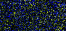
\includegraphics[width = .19\linewidth]{sb231_day_0}}
  \subcaptionbox{9 June\label{fig:day_24}}{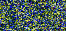
\includegraphics[width = .19\linewidth]{sb231_day_24}}
  \subcaptionbox{3 July\label{fig:day_48}}{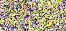
\includegraphics[width = .19\linewidth]{sb231_day_48}}
  \subcaptionbox{27 July\label{fig:day_72}}{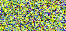
\includegraphics[width = .19\linewidth]{sb231_day_72}}
  \subcaptionbox{20 Aug.\label{fig:day_96}}{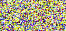
\includegraphics[width = .19\linewidth]{sb231_day_96}}
  \caption{Crop samples taken in 2016, in Pauli decomposition}
  \label{fig:sample_images}
\end{figure}

Fig.~\ref{fig:AllIndexes} shows estimates of the densities of the three Geodesic Indexes (Purity $P_{\text{GD}}$, Scattering Type Angle -- Alpha $\alpha_{\text{GD}}$, and Helicity $\tau_{\text{GD}}$) for the four crops (Canola, Oats, Soy Beans, and Wheat) in the five dates here considered.

\begin{figure*}[htb]
\centering
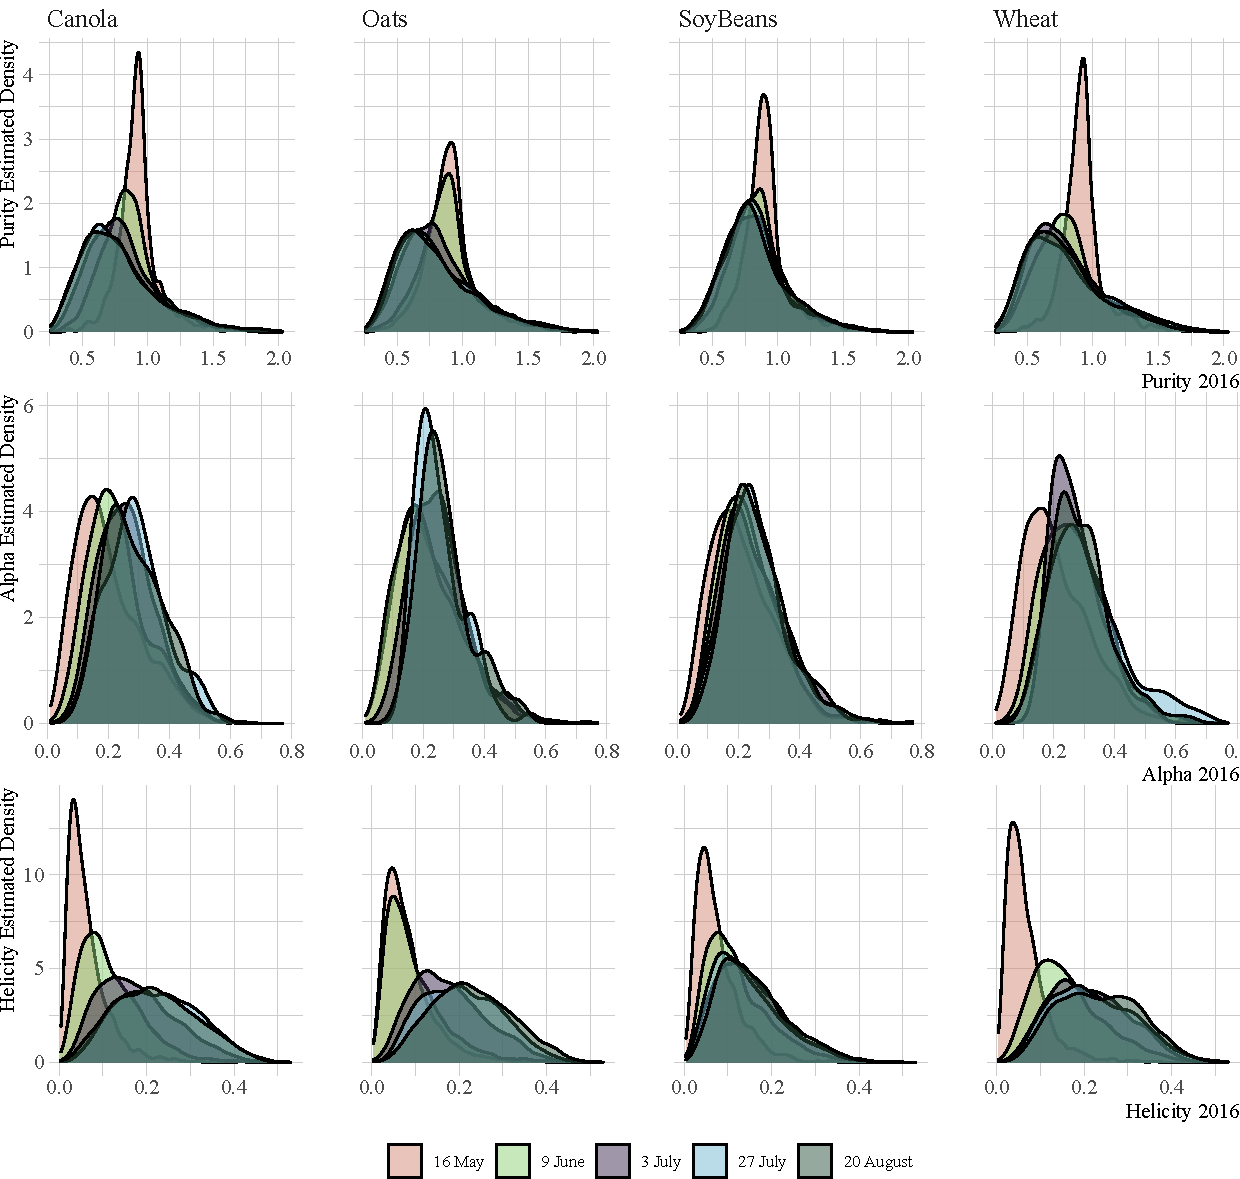
\includegraphics[width=.7\linewidth]{Indexes}
\caption{Density estimates of the three Geodesic Indexes by crop and date.}\label{fig:AllIndexes}
\end{figure*}

\subsection{Data Analysis}

\subsubsection{Geodesic Purity}

An exploratory data analysis revealed that the logarithmic transformation leads to data that can be well described by the Gaussian distribution.
We, thus, opted for fitting the Lognormal law, characterized by the probability density function
\begin{equation}
f(x;\mu,\sigma^2) = \frac{1}{\sqrt{2\pi\sigma^2} x} \exp\Big\{
-\frac1{2 \sigma^2}\big(\log x - \mu\big)^2
\Big\},
\end{equation}
where $\mu\in\mathbbm R$, and $\sigma^2>0$ are the parameters.

Table~\ref{tab:params_purity} shows the Maximum Likelihood estimates of the Lognormal model ($\widehat \mu,\widehat{\sigma^2}$), and $p$-value of the Anderson-Darling goodness-of-fit test for the Geodesic Purity $P_{\text{GD}}$.
All samples sizes are $n=1950$.
Notice that the minimum $p$-value is $0.076$; there is, thus, no evidence that the Lognormal models should not be used for these samples.
The Lognormal distribution has the additional advantage that it describes data which, after a logarithmic transformation, can be treated as Gaussian.
Fig.~\ref{fig:WorstPurityLognormalFit} shows the histogram of the data with the worst fit (Wheat, 16~May), and the fitted density; we used the Freedman-Diaconis rule to compute the number of bins.

\begin{table}[hbt]
	\centering
	\caption{Maximum Likelihood estimates of the Lognormal model ($\widehat \mu,\widehat{\sigma^2}$), and $p$-value of the Anderson-Darling goodness-of-fit test for the Geodesic Purity $P_{\text{GD}}$.}
	\label{tab:params_purity}
	\setlength{\tabcolsep}{2pt}
	\begin{tabular}{clrrrrr}
		\toprule
		\textbf{Crop $\backslash$ Date} & & \textbf{16 May} & \textbf{9 June} & \textbf{3 July} & \textbf{27 July} & \textbf{20 Aug.}\\ \cmidrule(lr){1-2} \cmidrule(lr){3-3} \cmidrule(lr){4-4} \cmidrule(lr){5-5} \cmidrule(lr){6-6} \cmidrule(lr){7-7}
		\textbf{Canola} 	
		& $\widehat{\mu}$ 		& $-0.0890$  & $-0.1738$   & $-0.2681$   & $-0.3187$   & $-0.3072$ \\
		& $\widehat{\sigma^2}$ 	& 0.0295 	& 0.0676 	& 0.0994 	& 0.1269  	& 0.1361 \\ 
		& $p$-value 			& 0.2701	& 0.2739 	& 0.7064 	& 0.5727 	& 0.7515\\		
		\midrule
		\textbf{Soy Beans}
		& $\widehat{\mu}$ 		& $-0.1120$	& $-0.1831$	& $-0.2356$ & $-0.2278$ & $-0.2350$         \\
		& $\widehat{\sigma^2}$ 	& 0.0334   	& 0.0670   	& 0.0859   	& 0.079   	& 0.0848 \\ 
		& $p$-value 			& 0.8921 	& 0.8273 	& 0.7992 	& 0.9841 	& 0.7099\\			
		\midrule
		\textbf{Oats}
		& $\widehat{\mu}$ 		& $-0.1223$ & $-0.1358$	& $-0.2578$ & $-0.2679$	& $-0.3008$ \\
		& $\widehat{\sigma^2}$ 	& 0.0479 	& 0.0737   	& 0.1085 	& 0.1267  	& 0.1338 \\ 
		& $p$-value 			& 0.8438 	& 0.1024 	& 0.8262 	& 0.7027	& 0.3977 \\
		\midrule
		\textbf{Wheat} 
		& $\widehat{\mu}$ 		& $-0.0947$	& $-0.2392$ & $-0.2866$ & $-0.2837$ & $-0.3145$ \\
		& $\widehat{\sigma^2}$ 	& 0.0310   	& 0.0972   	& 0.1099   	& 0.1461   	& 0.1269   \\
		& $p$-value 			& 0.0760 	& 0.5490 	& 0.3051 	& 0.4034 	& 0.4177\\	
		\bottomrule
	\end{tabular}
\end{table}

\begin{figure*}[hbt]
	\centering
\subcaptionbox{Geodesic Purity $P_{\text{GD}}$ from Wheat, 16~May, and fitted Lognormal density.\label{fig:WorstPurityLognormalFit}}{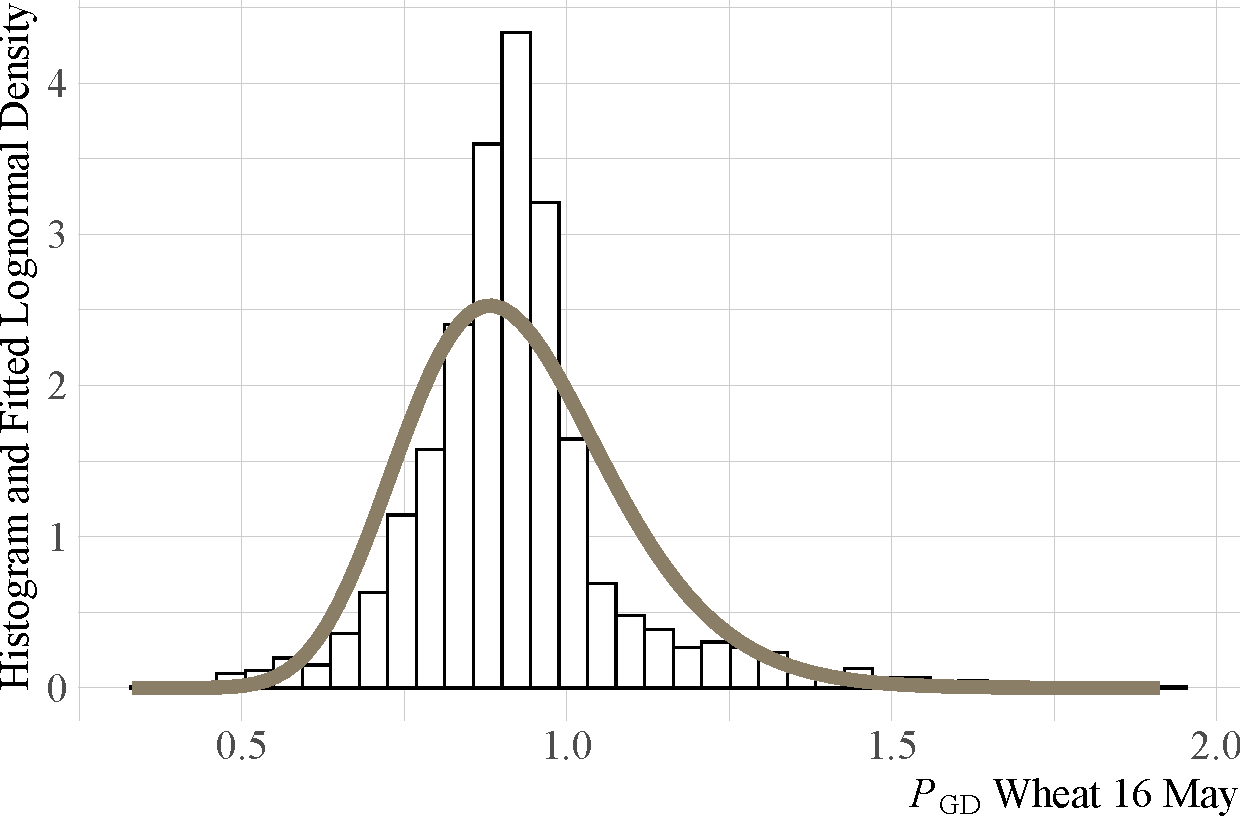
\includegraphics[width=.32\linewidth]{WheatPurityLognormalFit}}
%
\subcaptionbox{Geodesic Scattering Type Angle $\alpha_{\text{GD}}$ from Canola, 16~May, and fitted Beta density.\label{fig:WorstAlphaBetaFit}}{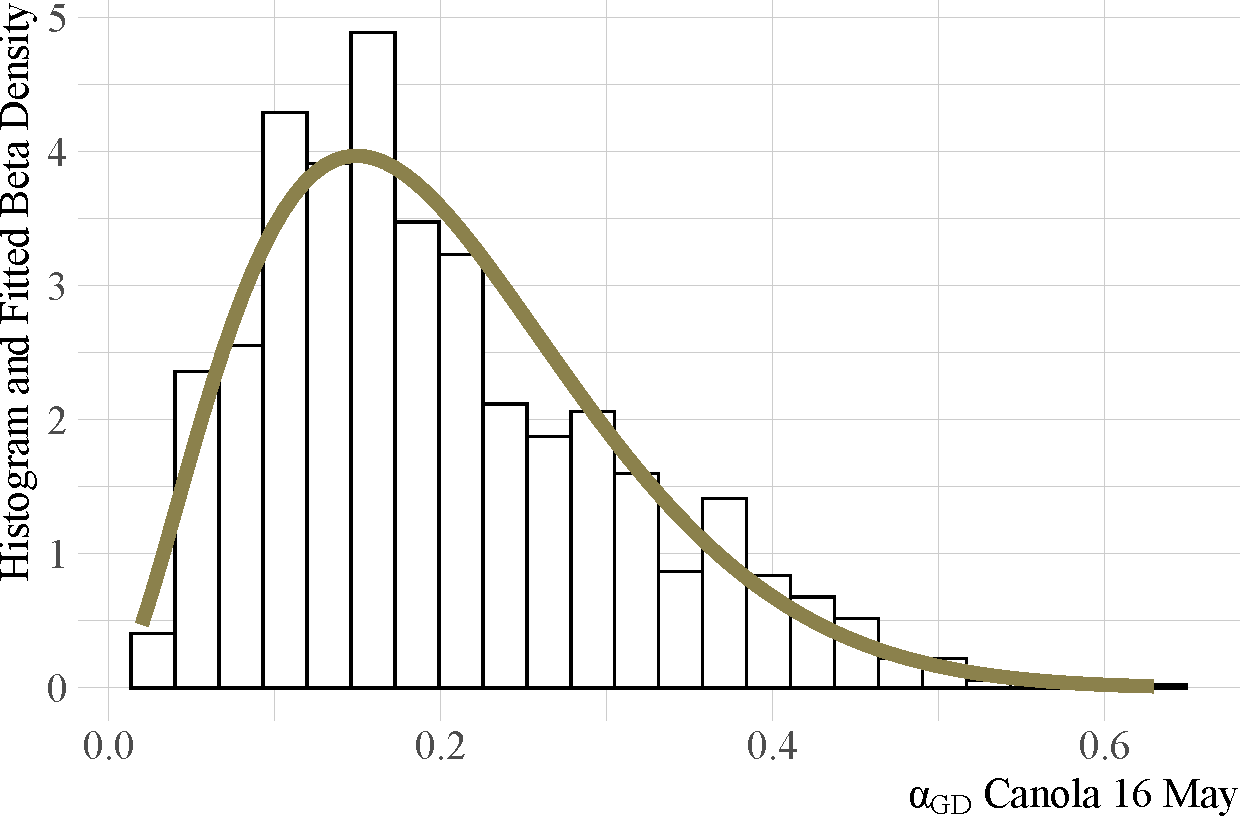
\includegraphics[width=.32\linewidth]{CanolaAlphaBetaFit}}
%
\subcaptionbox{Geodesic Helicity $\tau_{\text{GD}}$ from Canola, 16~May, and fitted Beta density.\label{fig:WorstHelicityBetaFit}}{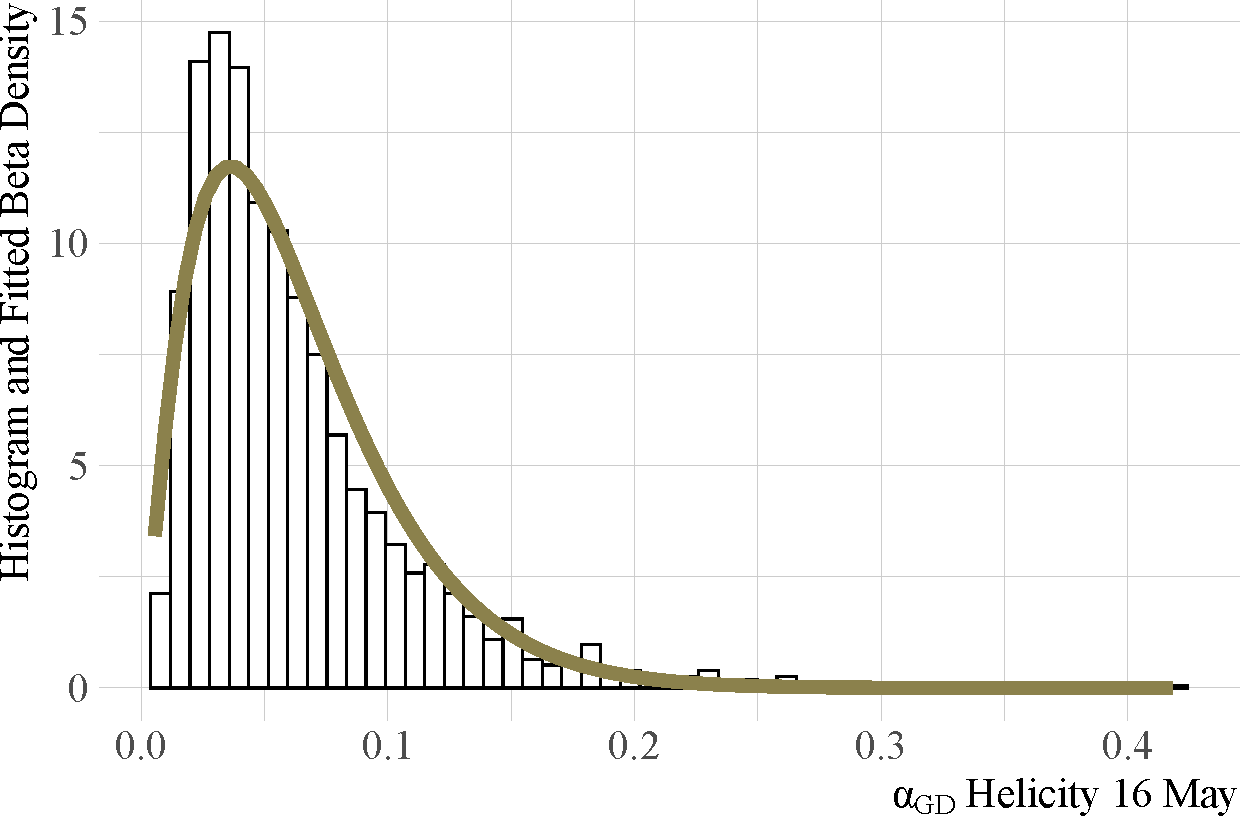
\includegraphics[width=.32\linewidth]{CanolaHelicityBetaFit}}
	\caption{The three worst fits of Geodesic indexes.}
\end{figure*}

\subsubsection{Geodesic Scattering Type Angle and Helicity}

The observations are bounded in $(0,1)$, 
and the shape of their estimated densities also suggests the use of the Beta distribution, characterized by the probability density function:
\begin{equation}
f(x; p, q) = \frac{\Gamma(p+q)}{\Gamma(p)\Gamma(q)} x^{p-1} (1-x)^{q-1} \mathbbm 1_{(0,1)}(x),
\label{eq:BetaDensity}
\end{equation}
with $p,q>0$.
%The data look crammed in their original space, though, and then we decided to assess the observations after a logarithmic transformation.
%Fig.~\ref{fig:histograms_purity_sb231} shows the histograms and boxplots. 

For $\alpha_{\text{GD}}$, we computed the distance of each pixel to all prototypes (except to $\bm K_{\text{ID}}$), and retained those closer to $\bm K_{\text{t}}$ than to the others.

Table~\ref{tab:params_alpha} shows, for each crop type and date, 
the sample size ($n$), 
the Maximum Likelihood estimates of the Beta model ($\widehat p,\widehat q$), and the $p$-value of the Kolmogorov-Smirnof goodness-of-fit test for the Geodesic Scattering Type Angle $\alpha_{\text{GD}}$.
Notice that, although the minimum $p$-value is $0.0103$, the others range between $0.0723$ and $0.9887$; there is, thus, no evidence that the Beta models should not be used for these samples.
Fig.~\ref{fig:WorstAlphaBetaFit} shows the histogram of the data with the worst fit (Canola, 16~May), and the fitted density; we used the Freedman-Diaconis rule to compute the number of bins.

\begin{table}[hbt]
	\centering
	\caption{Sample size ($n$), Maximum Likelihood estimates of the Beta model ($\widehat p,\widehat q$), and $p$-value of the Kolmogorov-Smirnof goodness-of-fit test for the Geodesic Scattering Type Angle $\alpha_{\text{GD}}$.}
	\label{tab:params_alpha}
	\setlength{\tabcolsep}{3.8pt}
\begin{tabular}{clrrrrr}
	\toprule
\textbf{Crop $\backslash$ Date} & & \textbf{16 May} & \textbf{9 June} & \textbf{3 July} & \textbf{27 July} & \textbf{20 Aug.}\\ \cmidrule(lr){1-2} \cmidrule(lr){3-3} \cmidrule(lr){4-4} \cmidrule(lr){5-5} \cmidrule(lr){6-6} \cmidrule(lr){7-7}
\textbf{Canola} 	& $n$ 			& 1389 		& 730 		& 333 		& 130 		& 145\\
 		& $\widehat{p}$ & 2.7560 	& 4.1886 	& 5.8105 	& 6.1547 	& 6.3503\\
		& $\widehat{q}$ & 11.0141 	& 13.9375 	& 16.4850 	& 15.1480 	& 15.9220\\ 
 		& $p$-value 	& 0.0103 	& 0.2955 	& 0.9887 	& 0.9503 	& 0.6245\\		
		\midrule
\textbf{Soy Beans}	& $n$ 			& 1285 		& 656 		& 449 		& 615 		& 508\\
 			& $\widehat{p}$ & 3.2348 	& 4.3843 	& 4.0188 	& 4.8295 	& 5.1401\\
			& $\widehat{q}$ & 11.9960 	& 14.4563 	& 11.8697 	& 14.2715 	& 14.5409\\ 
 			& $p$-value 	& 0.5666 	& 0.4052 	& 0.1814 	& 0.2687 	& 0.3187\\			
			\midrule
\textbf{Oats}	& $n$ 			& 1207 		& 991 		& 263 		& 82 		& 66\\
		& $\widehat{p}$ & 3.2822  	& 3.1221 	& 5.2792 	& 8.0549 	& 7.5261\\
		& $\widehat{q}$ & 11.1652 	& 10.9882 	& 15.7778 	& 23.9306 	& 20.3871\\ 
		& $p$-value 	& 0.1300 	& 0.1526 	& 0.4645 	& 0.1992 	& 0.3646\\
		\midrule
\textbf{Wheat} 	& $n$ 			& 1382 		& 413 		& 131 		& 122 		& 116\\
		& $\widehat{p}$ & 2.9096  	& 4.8869 	& 8.4877 	& 4.5926 	& 6.1919\\
		& $\widehat{q}$ & 10.9248 	& 13.4887 	& 21.9157 	& 10.1156 	& 15.3390\\
		& $p$-value 	& 0.0723 	& 0.7890 	& 0.3638 	& 0.2067 	& 0.7346\\	
	\bottomrule
\end{tabular}
\end{table}

Table~\ref{tab:params_helicity} shows the Maximum Likelihood estimates of the Beta model ($\widehat p,\widehat q$), and $p$-value of the Kolmogorov-Smirnof goodness-of-fit test for the Geodesic Helicity $\tau_{\text{GD}}$.
All samples sizes are $n=1950$.
Although the $p$-value of five out of twenty samples falls below \SI{1}{\percent}, they are all larger than \SI{1}{\pertenmille}.
We, thus, have no strong evidence against the Beta model for describing the Geodesic Helicity.
Fig.~\ref{fig:WorstHelicityBetaFit} shows the histogram of the data with the worst fit (Canola, 16~May), and the fitted density; we used the Freedman-Diaconis rule to compute the number of bins.

\begin{table}[hbt]
	\centering
	\caption{Maximum Likelihood estimates of the Beta model ($\widehat p,\widehat q$), and $p$-value of the Kolmogorov-Smirnof goodness-of-fit test for the Geodesic Helicity $\tau_{\text{GD}}$.}
	\label{tab:params_helicity}
	\setlength{\tabcolsep}{3.8pt}
	\begin{tabular}{clrrrrr}
		\toprule
		\textbf{Crop $\backslash$ Date} & & \textbf{16 May} & \textbf{9 June} & \textbf{3 July} & \textbf{27 July} & \textbf{20 Aug.}\\ \cmidrule(lr){1-2} \cmidrule(lr){3-3} \cmidrule(lr){4-4} \cmidrule(lr){5-5} \cmidrule(lr){6-6} \cmidrule(lr){7-7}
		\textbf{Canola} 	
		& $\widehat{p}$ & 2.1856  	& 2.6837    & 5.8105 	& 3.3877  	& 4.4111 \\
		& $\widehat{q}$ & 32.5176 	& 20.3264 	& 16.4850 	& 15.5491 	& 14.9766\\ 
		& $p$-value 	& 1E$-4$ 		& 0.0645 	& 0.9887 	& 0.3356 	& 0.0166\\		
		\midrule
		\textbf{Soy Beans}
		& $\widehat{p}$ & 2.4317   	& 2.7304   	& 3.0602   	& 2.9543   	& 3.4111 \\
		& $\widehat{q}$ & 30.1012   & 19.8095   & 17.1821   & 17.7749   & 18.2627 \\ 
		& $p$-value 	& 5E$-4$ 	& 0.005 	& 0.9388 	& 0.0514 	& 0.1081\\			
		\midrule
		\textbf{Oats}
		& $\widehat{p}$ & 2.3701   	& 2.1838  	& 3.529     & 4.2011 	& 4.7568 \\
		& $\widehat{q}$ & 26.5330 	& 20.4121   & 16.4932 	& 16.1089  	& 15.9517 \\ 
		& $p$-value 	& 0.0016 	& 1E$-4$ 	& 0.541 	& 0.0078	& 0.1757 \\
		\midrule
		\textbf{Wheat} 
		& $\widehat{p}$ & 2.3516   	& 3.3384  	& 4.3960  	& 4.1996  	& 4.6823   \\
		& $\widehat{q}$ & 33.4388   & 17.1858   & 16.6094   & 14.8613   & 15.2931   \\
		& $p$-value 	& 5E$-4$ 	& 0.2118 	& 0.0476 	& 0.0215 	& 1E$-4$\\	
		\bottomrule
	\end{tabular}
\end{table}

\section{Temporal Evolution}

We first checked the hypothesis that every pair of parameters from the same crop in different dates comes from different models.
We used test statistics based on the Hellinger distance between the models~\cite{AnalyticExpressionsStochasticDistancesBetweenRelaxedComplexWishartDistributions}, and found that all the pairs are identifiable with \SI{5}{\percent} of significance, with the sole exception of $P_{\text{GD}}$ from Soy Beans in the two last dates.

Fig.~\ref{fig:TemporalIndexes} (top) shows the temporal evolution of the parameter estimates $(\widehat\mu,\widehat\sigma)$ of the Lognormal distribution when describing the Geodesic Purity index $P_{\text{GD}}$.
Canola, Oats, Soy Beans, and Wheat share similar behavior: $\widehat\mu$ decreases, while $\widehat\sigma$ increases with time, with the exception of the two last dates for Canola and Wheat.
The stages of these four crops are easily identifiable by means of the Lognormal model, whereas Soy Beans have only four identifiable stages since, as noted, the estimates from the two last dates cannot be considered different.

Fig.~\ref{fig:TemporalIndexes} (middle) shows the temporal evolution of the parameter estimates $(\widehat p, \widehat q)$ of the Beta distribution when modeling the Geodesic Scattering Type $\alpha_{\text{GD}}$.
Wheat is the crops where the estimates span most of the parametric space, as opposed to Soy Beans that gather around small values.
Although all estimates are significantly different, the two first dates of Oats are very close.

The estimates $(\widehat p, \widehat q)$ of the Beta distribution for the Geodesic Helicity $\tau_{\text{GD}}$ (Fig.~\ref{fig:TemporalIndexes} bottom) suggest a decreasing tendency of $\widehat q$ along with an increasing trend of $\widehat p$ along time.

\begin{figure*}
\centering
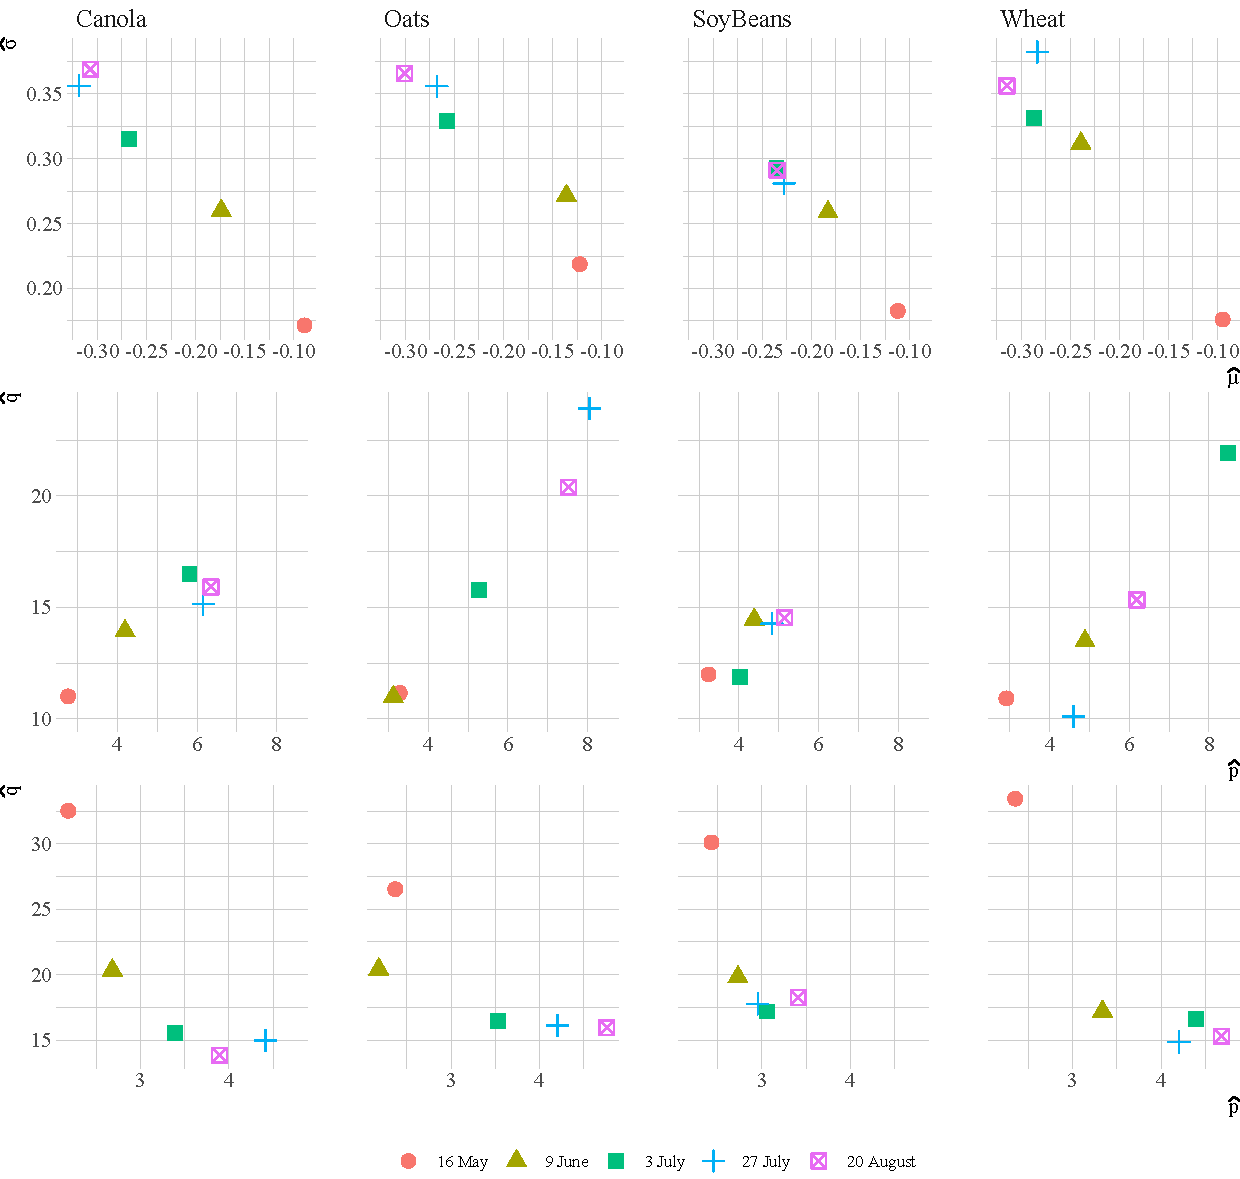
\includegraphics[width=.7\linewidth]{TemporalIndexes}
\caption{Temporal evolution of the parameter estimates $(\widehat\mu,\widehat\sigma)$ of the Lognormal distribution for the Geodesic Purity ($P_{\text{GD}}$, top), and of $(\widehat p,\widehat q)$ of the Beta distribution for the Geodesic Scattering Type Angle ($\alpha_{\text{GD}}$, middle) and Helicity ($\tau_{\text{GD}}$, bottom).}\label{fig:TemporalIndexes}
\end{figure*}
%
%\begin{figure*}
%	\centering
%	\includegraphics[width=.7\linewidth]{TemporalBetaScatteringTypeAngleParameters}
%	\caption{Temporal evolution of the parameter estimates $(\widehat p,\widehat q)$ of the Beta distribution for the Geodesic Scattering Type Angle index.}\label{fig:TemporalAlpha}
%\end{figure*}
%
%\begin{figure*}
%	\centering
%	\includegraphics[width=.7\linewidth]{TemporalBetaHelicityParameters}
%	\caption{Temporal evolution of the parameter estimates $(\widehat p,\widehat q)$ of the Beta distribution for the Geodesic Helicity index.}\label{fig:TemporalHelicity	}
%\end{figure*}

 
% The closeness to Gaussian distributions is remarkable.
% The QQ-Plots shown in Fig.~\ref{fig:qqplots} provide more evidence of such good adherence.
% Table~\ref{tab:pvalues_purities_sb231} provides the $p$-values of the Shapiro-Wilk test of goodness-of-fit to the Gaussian distribution.
% There is no evidence, thus, to reject the hypothesis that the log-transformed purity data follows Gaussian distributions.

% \begin{figure}[hbt]
%     \centering
%     \subcaptionbox{16 May 2016}{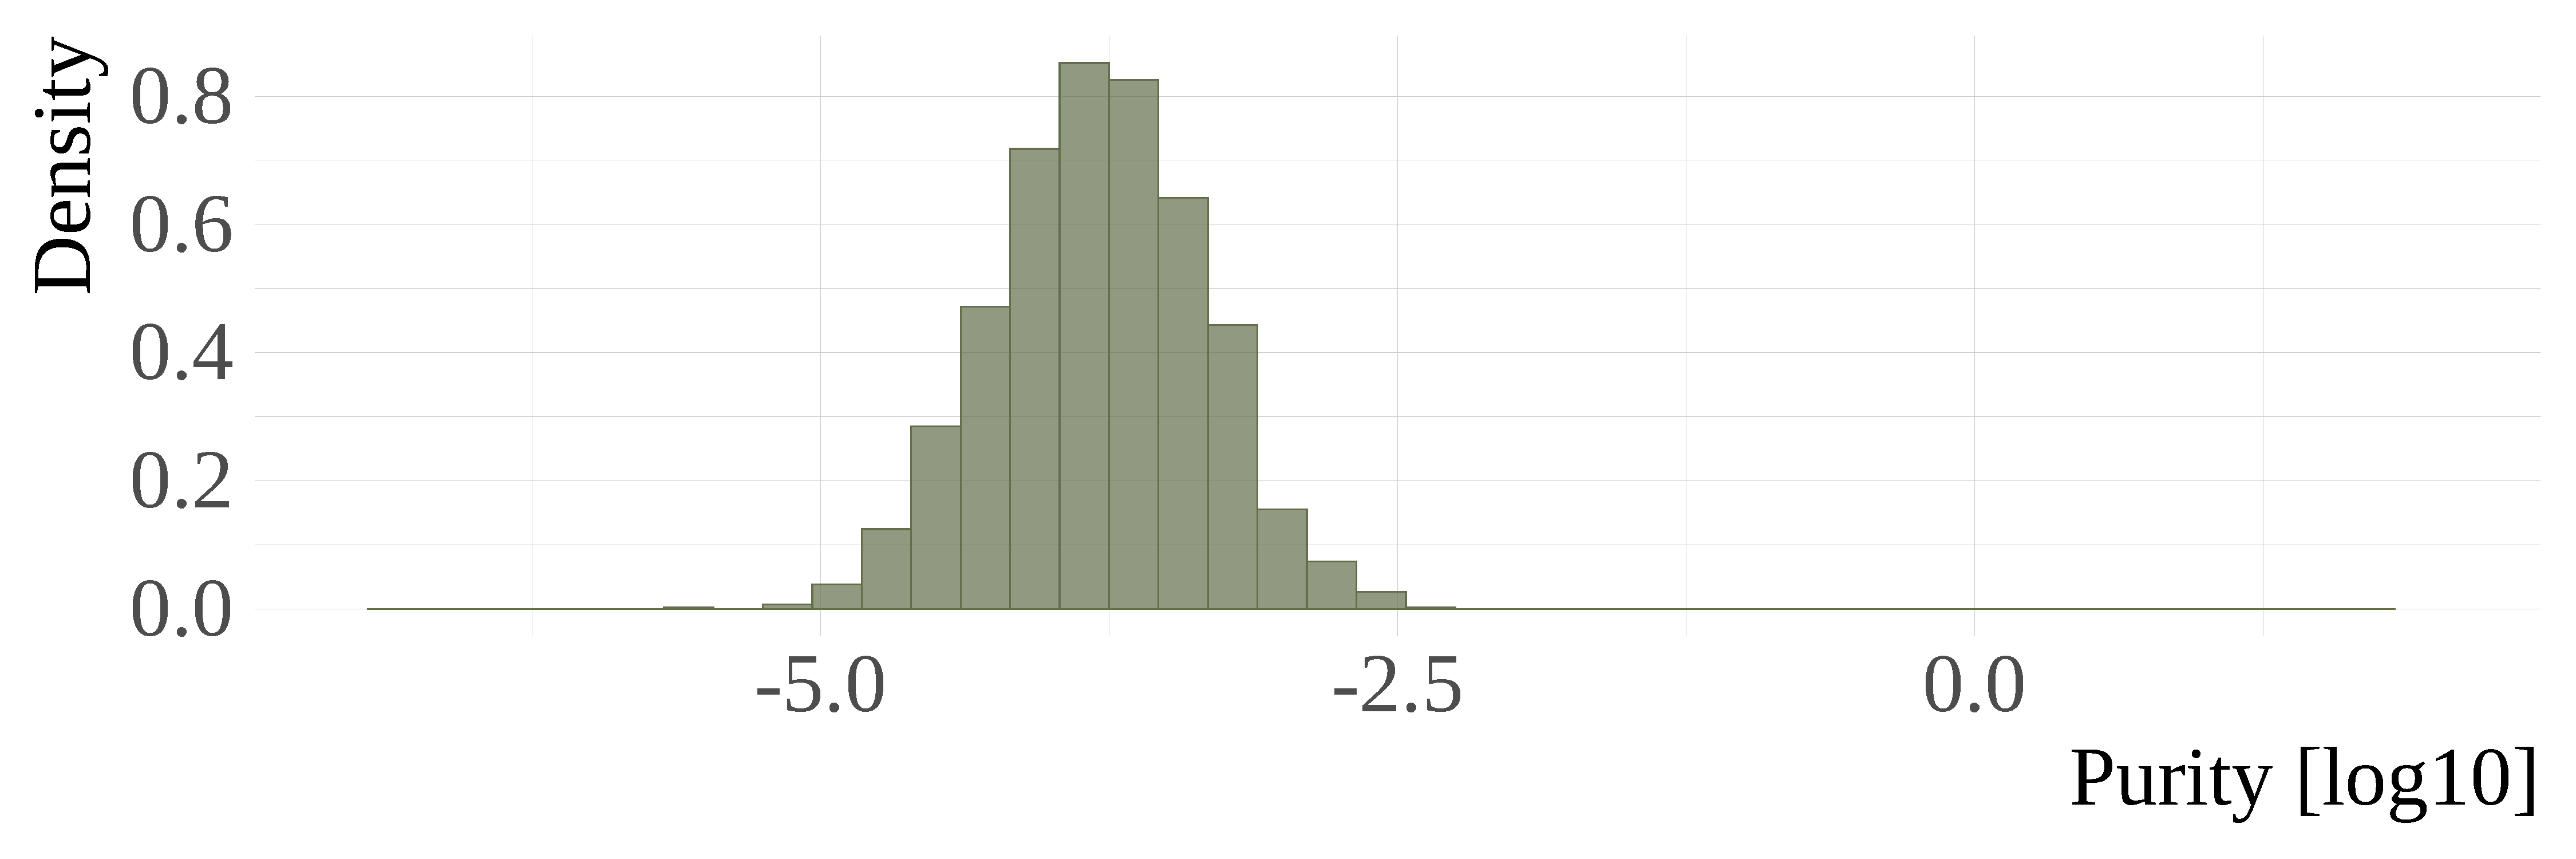
\includegraphics[width = \linewidth]{log_purity_sb231_1}}
%     \subcaptionbox{09 June 2016}{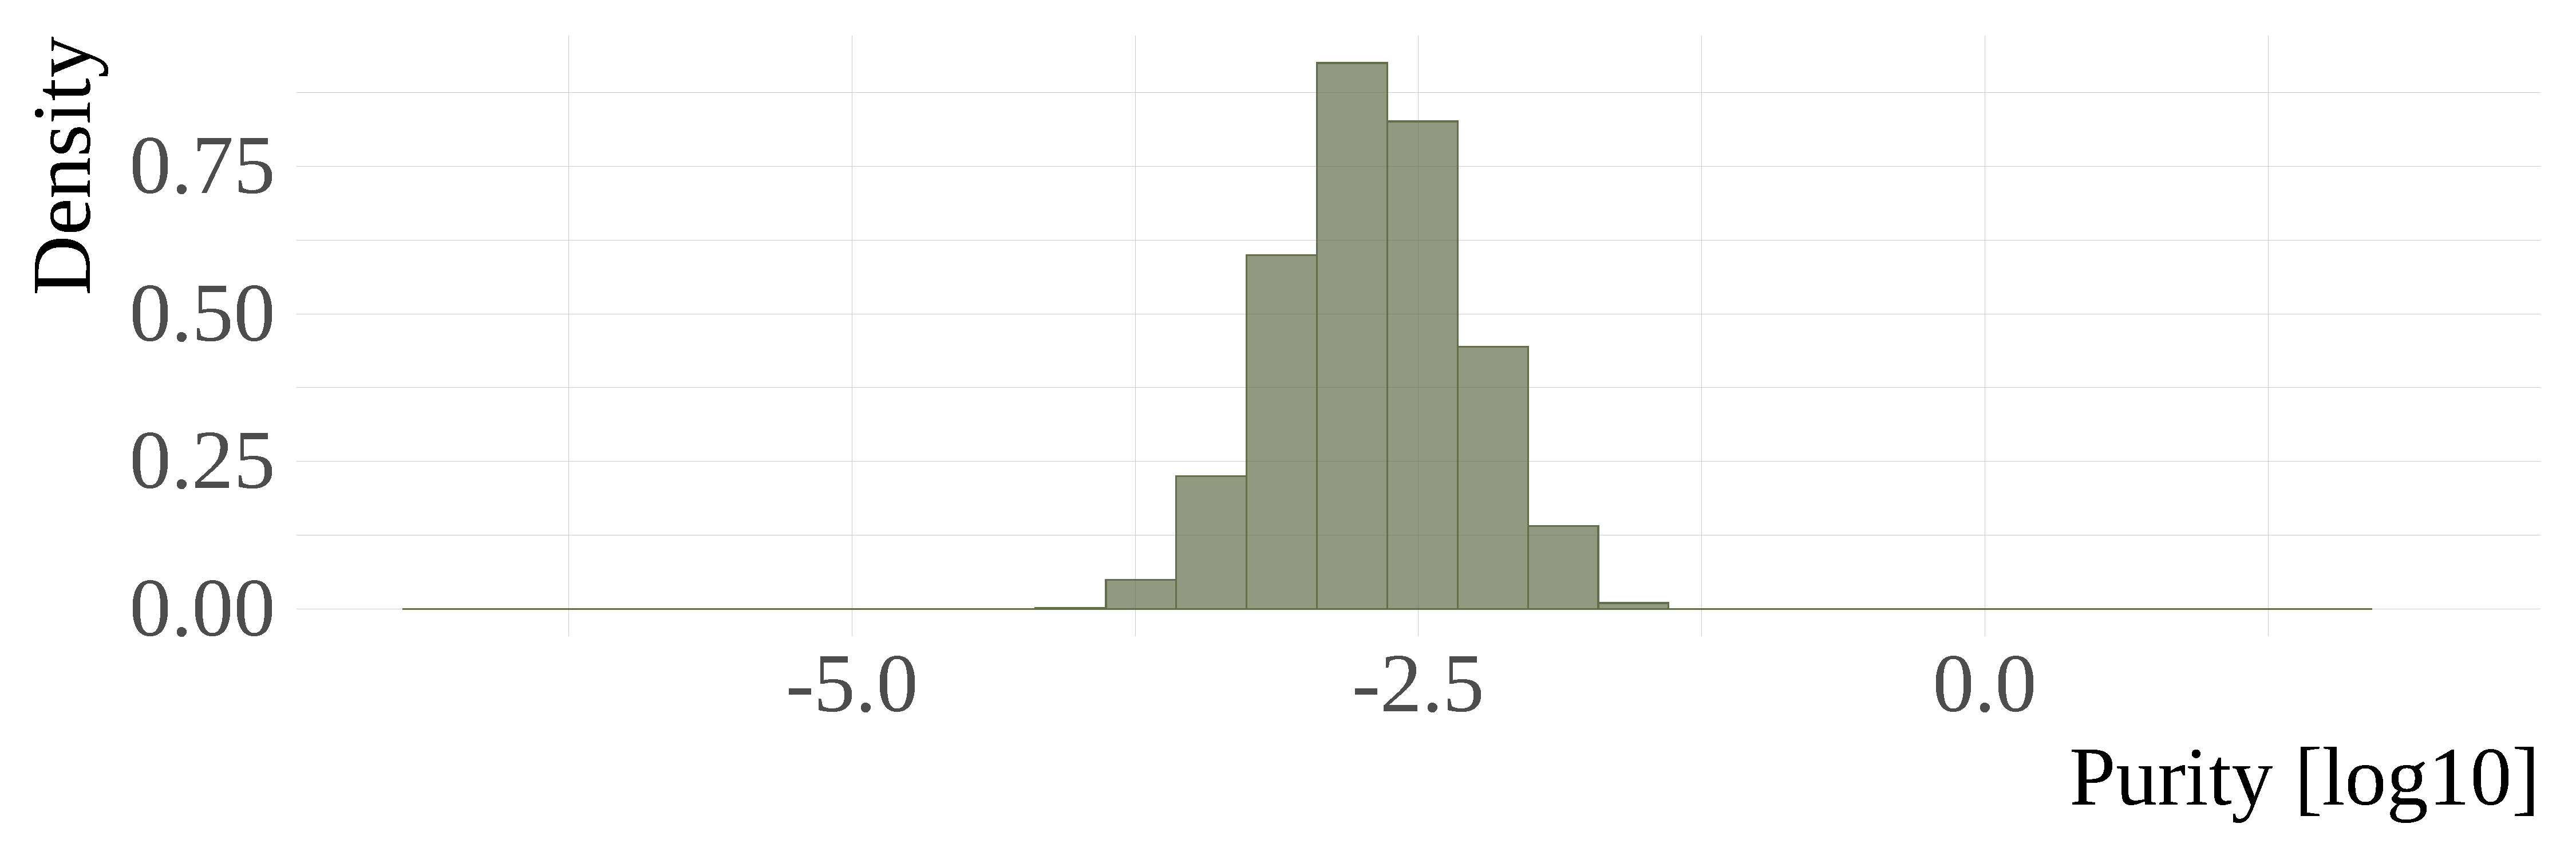
\includegraphics[width = \linewidth]{log_purity_sb231_2}}
%     \subcaptionbox{03 July 2016}{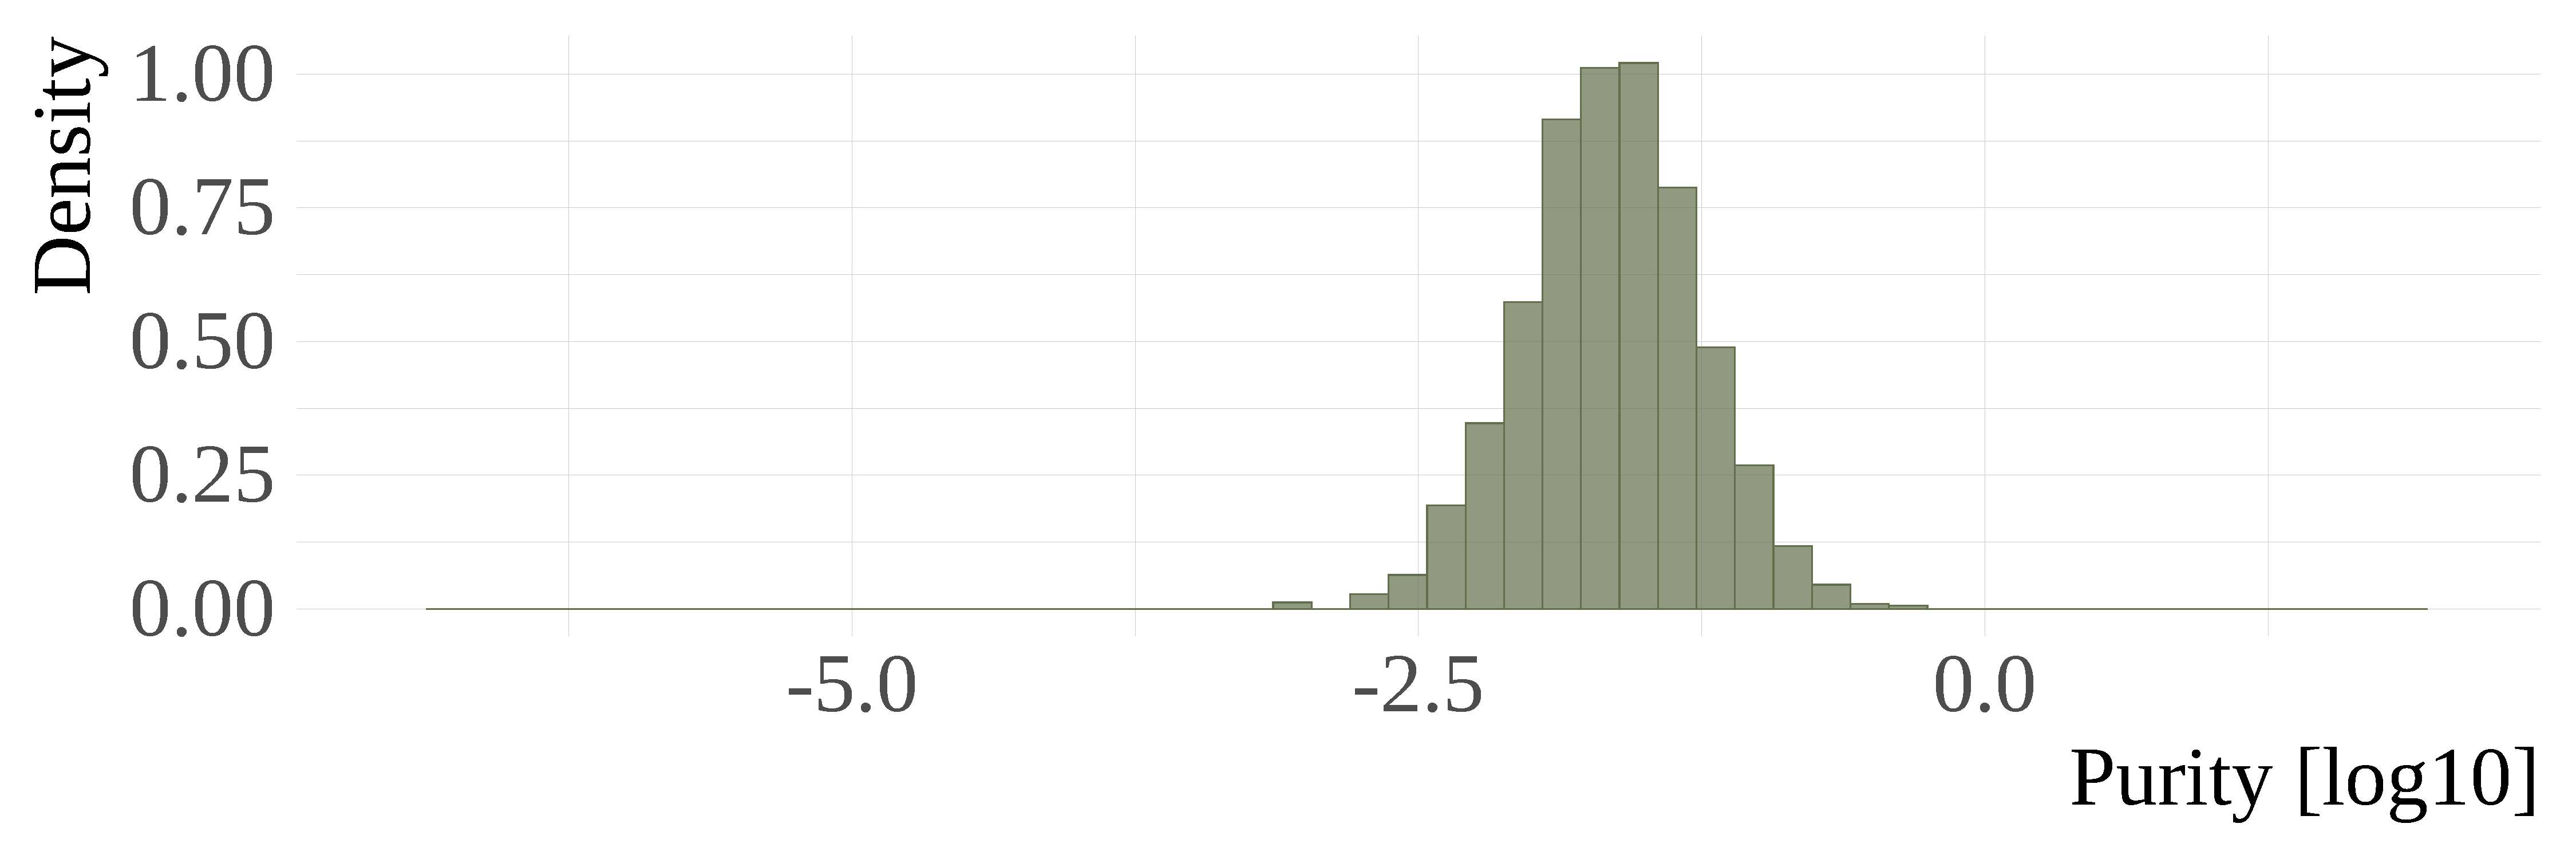
\includegraphics[width = \linewidth]{log_purity_sb231_3}}
%     \subcaptionbox{27 July 2016}{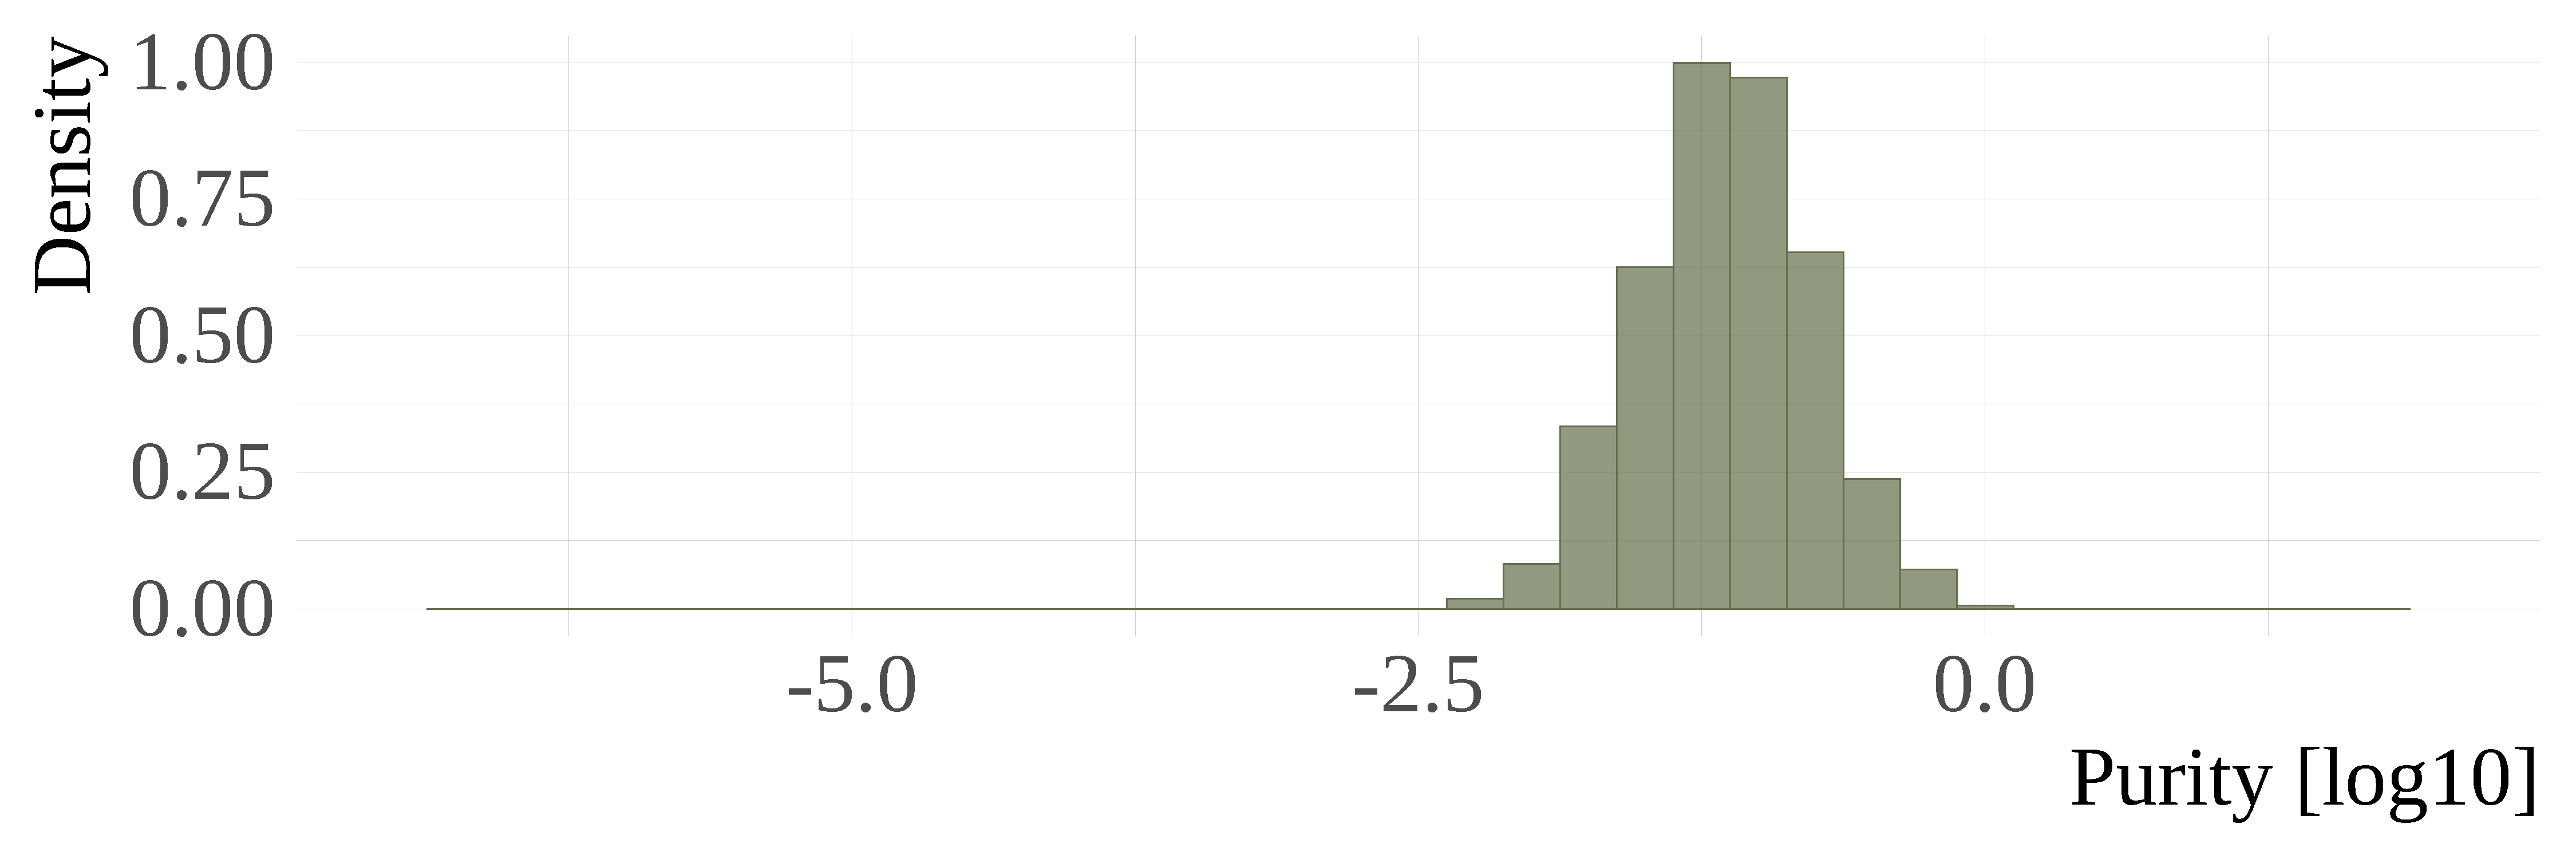
\includegraphics[width = \linewidth]{log_purity_sb231_4}}
%     \subcaptionbox{20 August 2016}{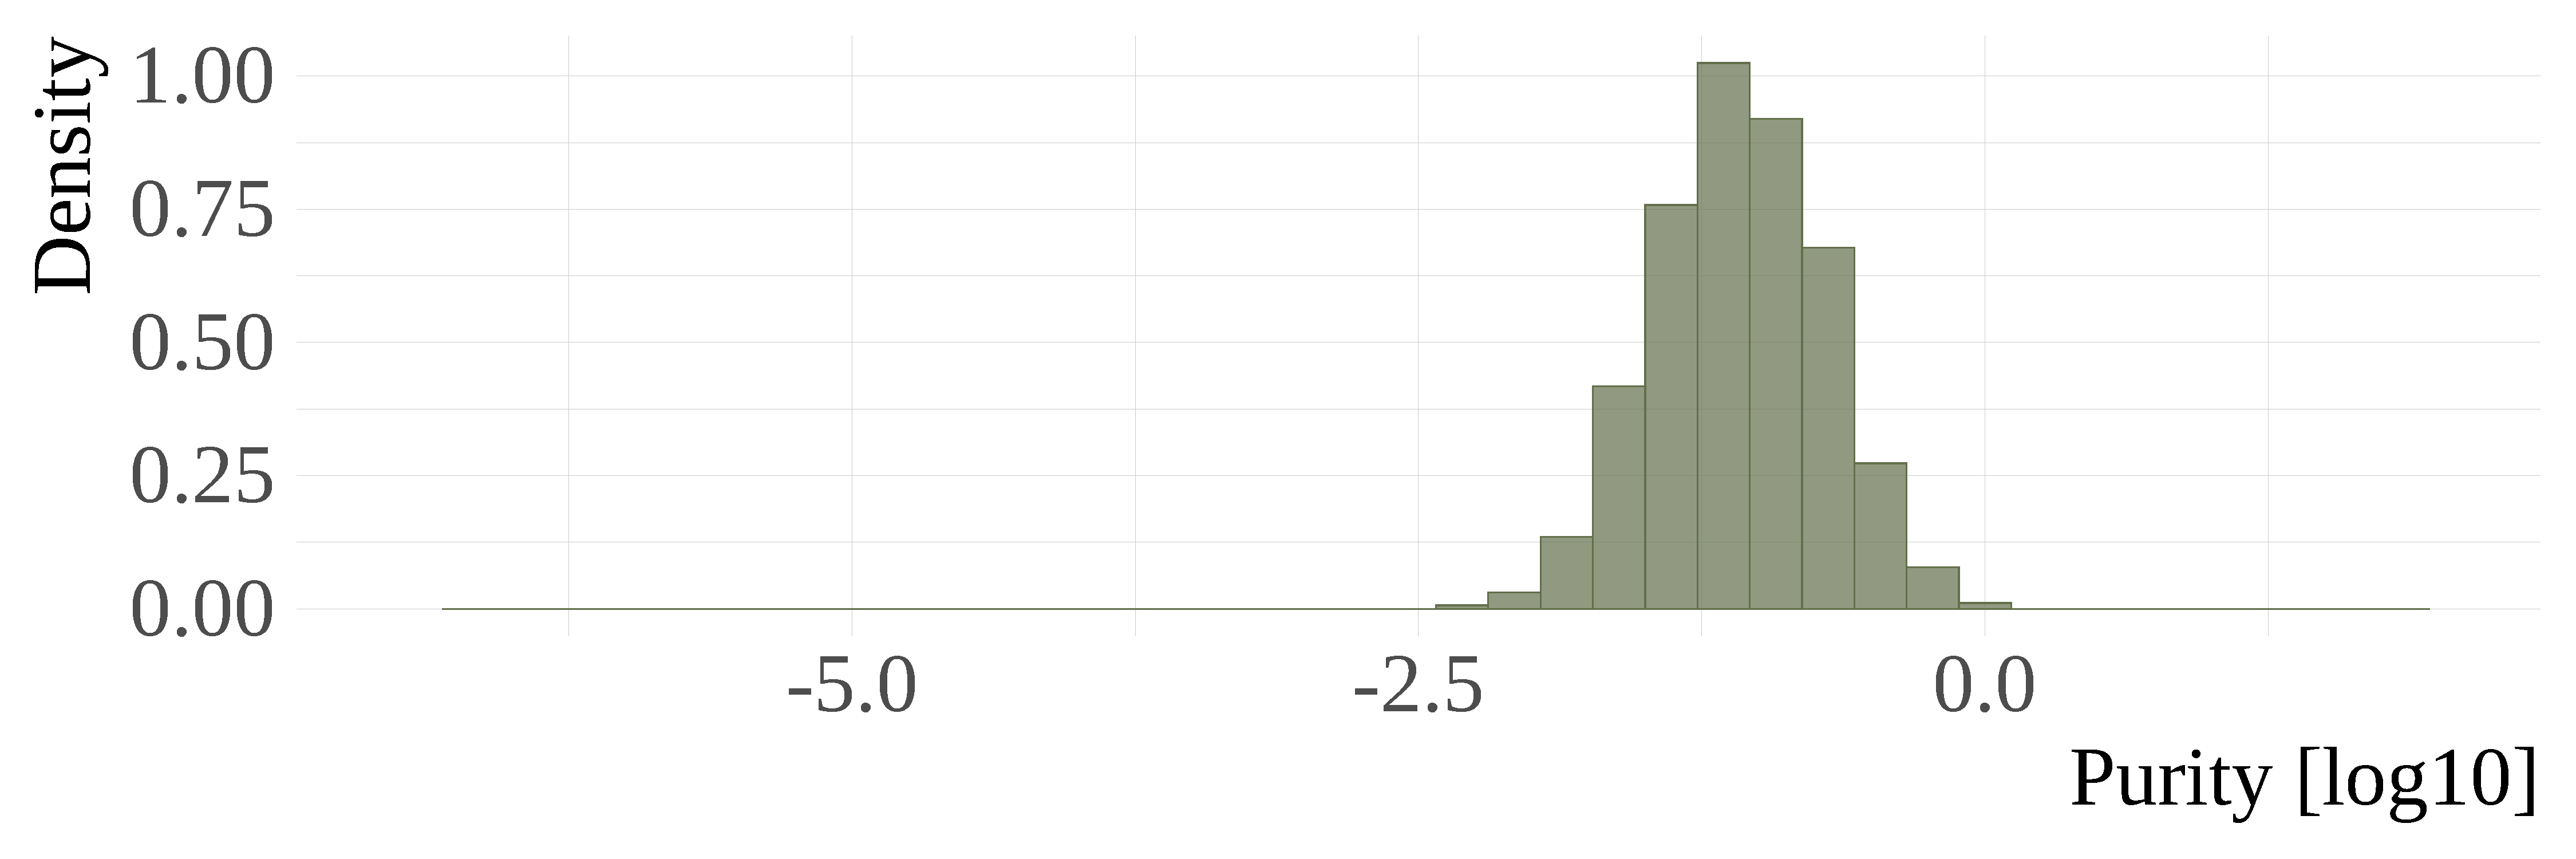
\includegraphics[width = \linewidth]{log_purity_sb231_5}}
%     \caption{Histograms of the $log10$ of geodesic purity index from Soybeans 231}
%     \label{fig:histograms_purity_sb231}
% \end{figure}

% \begin{figure}[hbt]
%     \centering
%     \subcaptionbox{16 May 2016}{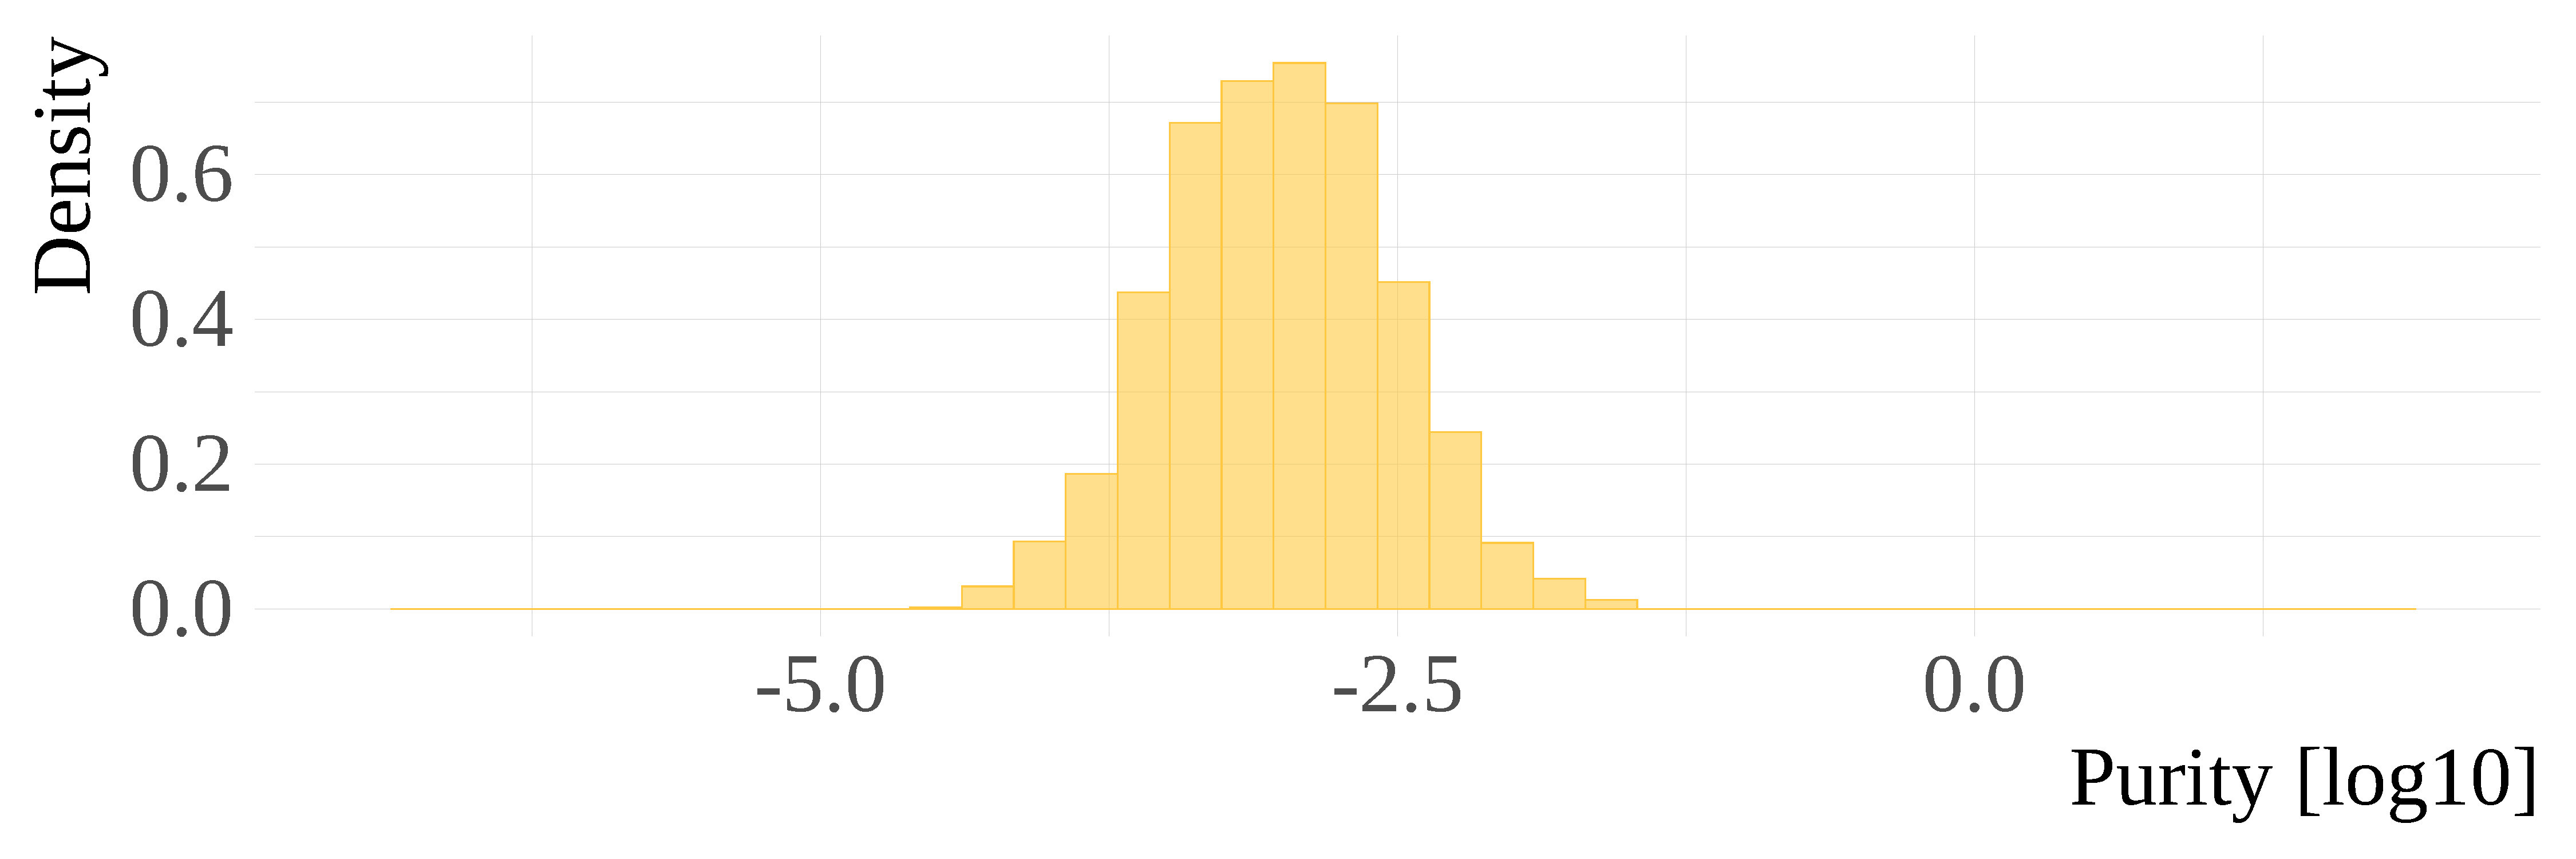
\includegraphics[width = \linewidth]{Figures/Canola_43/log_purity_cn43_1}}
%     \subcaptionbox{09 June 2016}{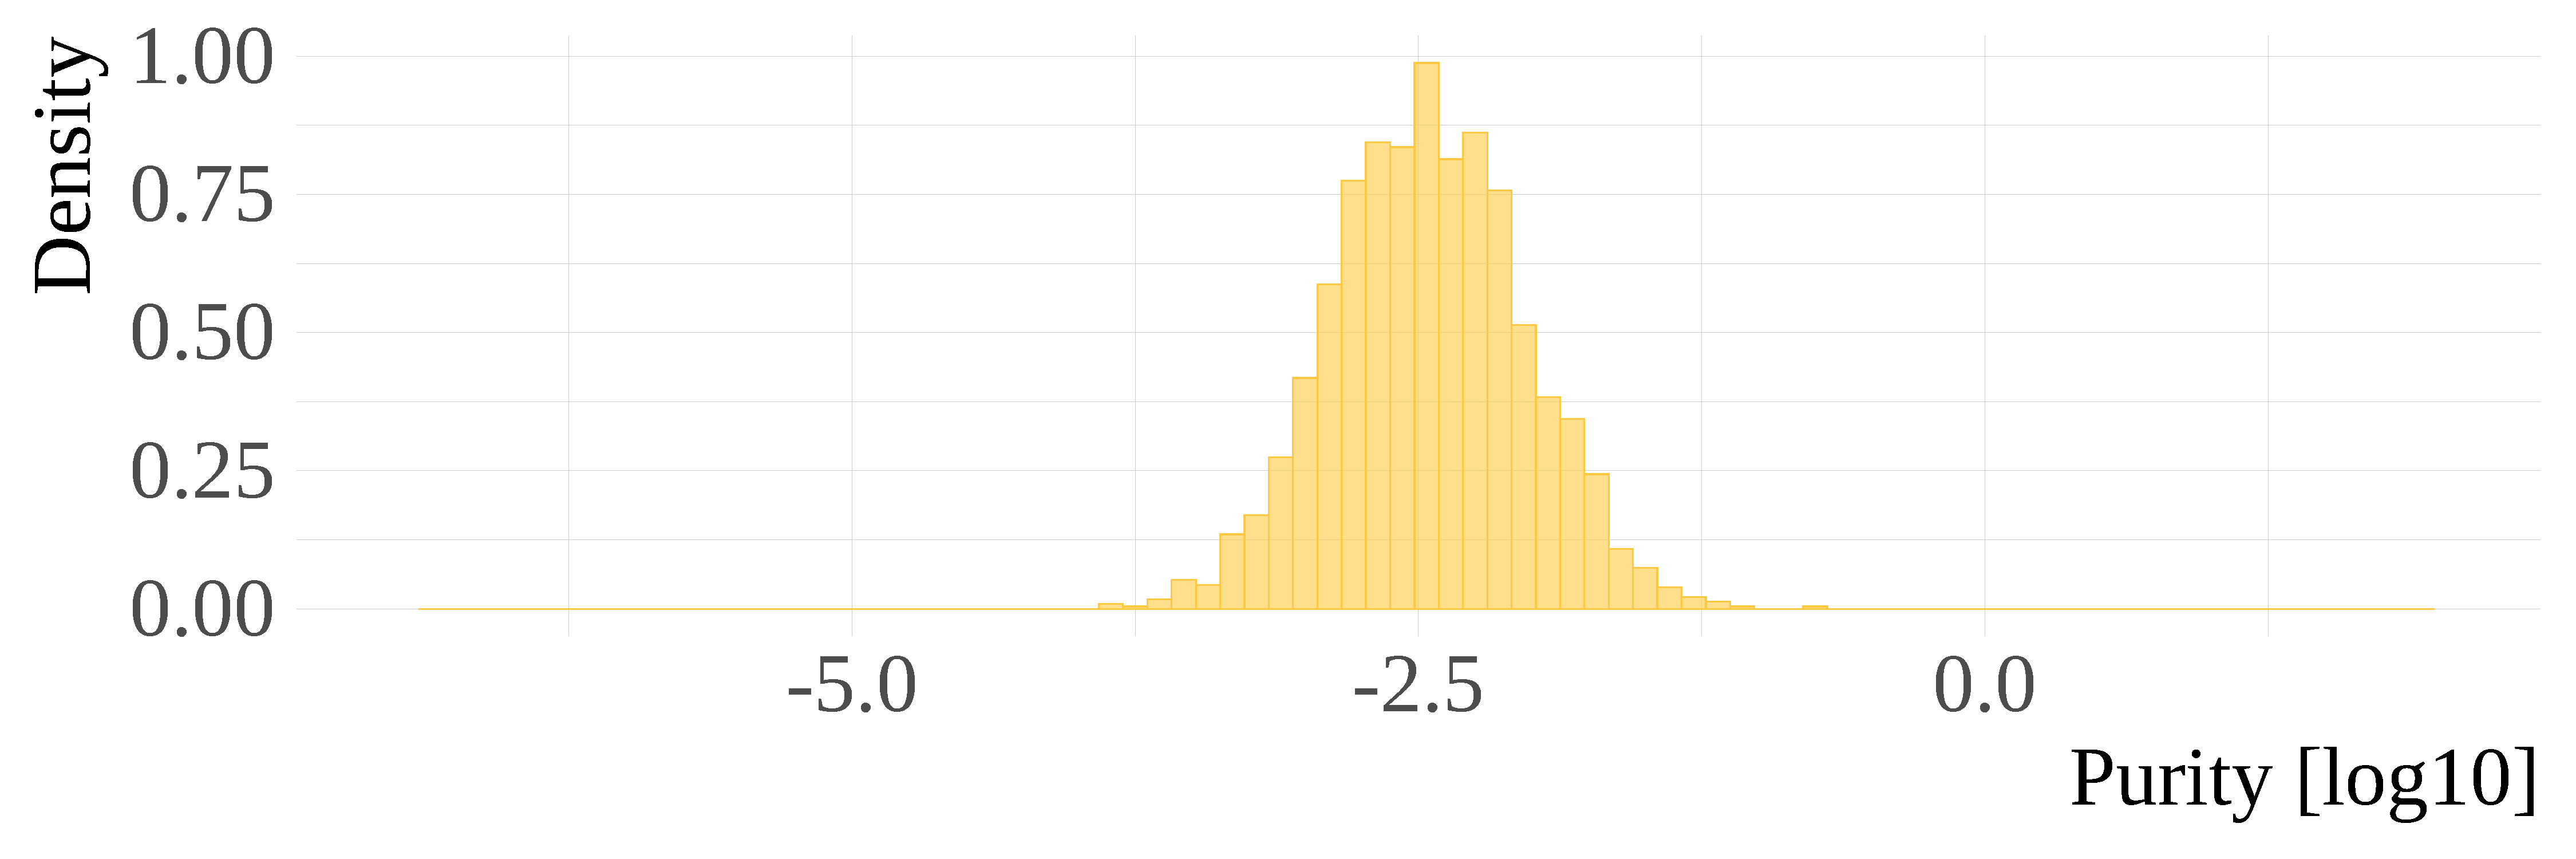
\includegraphics[width = \linewidth]{Figures/Canola_43/log_purity_cn43_2}}
%     \subcaptionbox{03 July 2016}{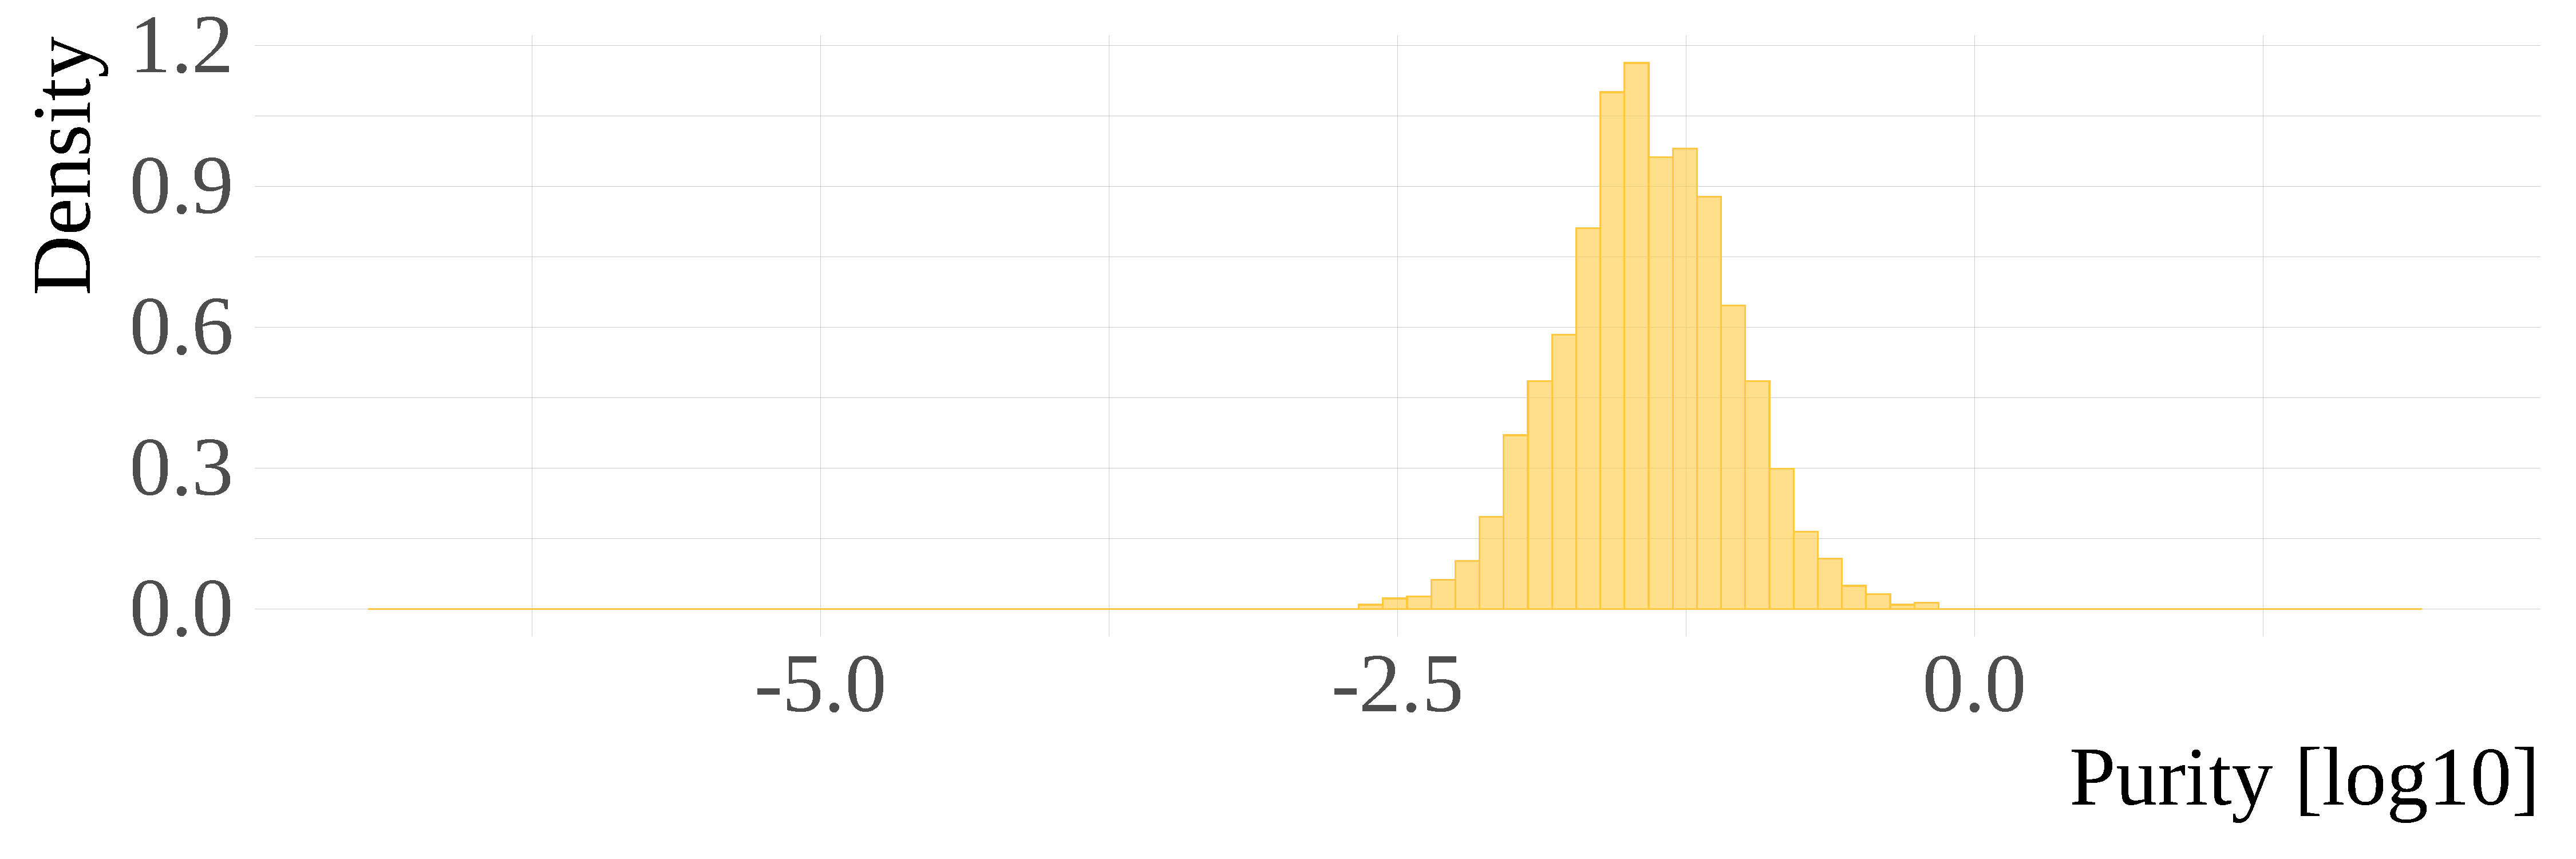
\includegraphics[width = \linewidth]{Figures/Canola_43/log_purity_cn43_3}}
%     \subcaptionbox{27 July 2016}{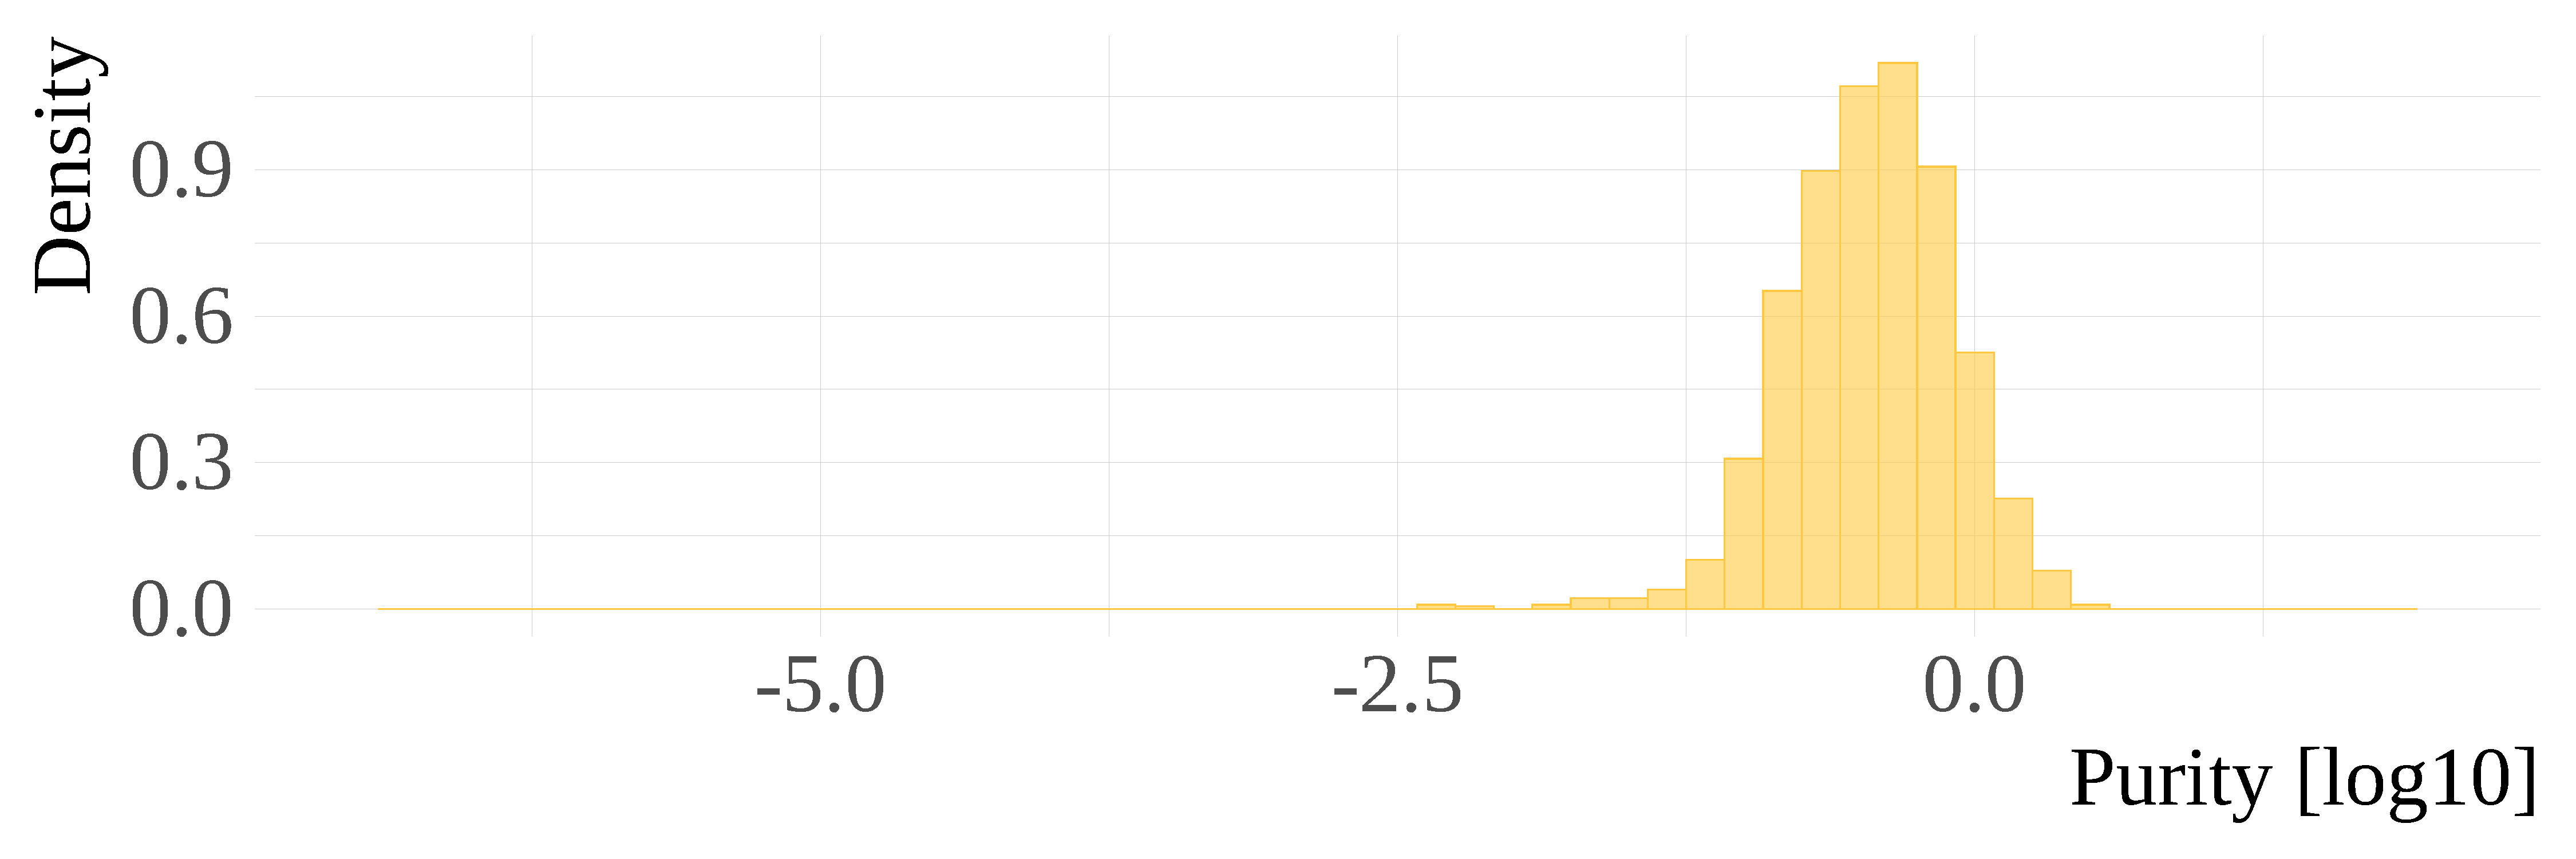
\includegraphics[width = \linewidth]{Figures/Canola_43/log_purity_cn43_4}}
%     \subcaptionbox{20 August 2016}{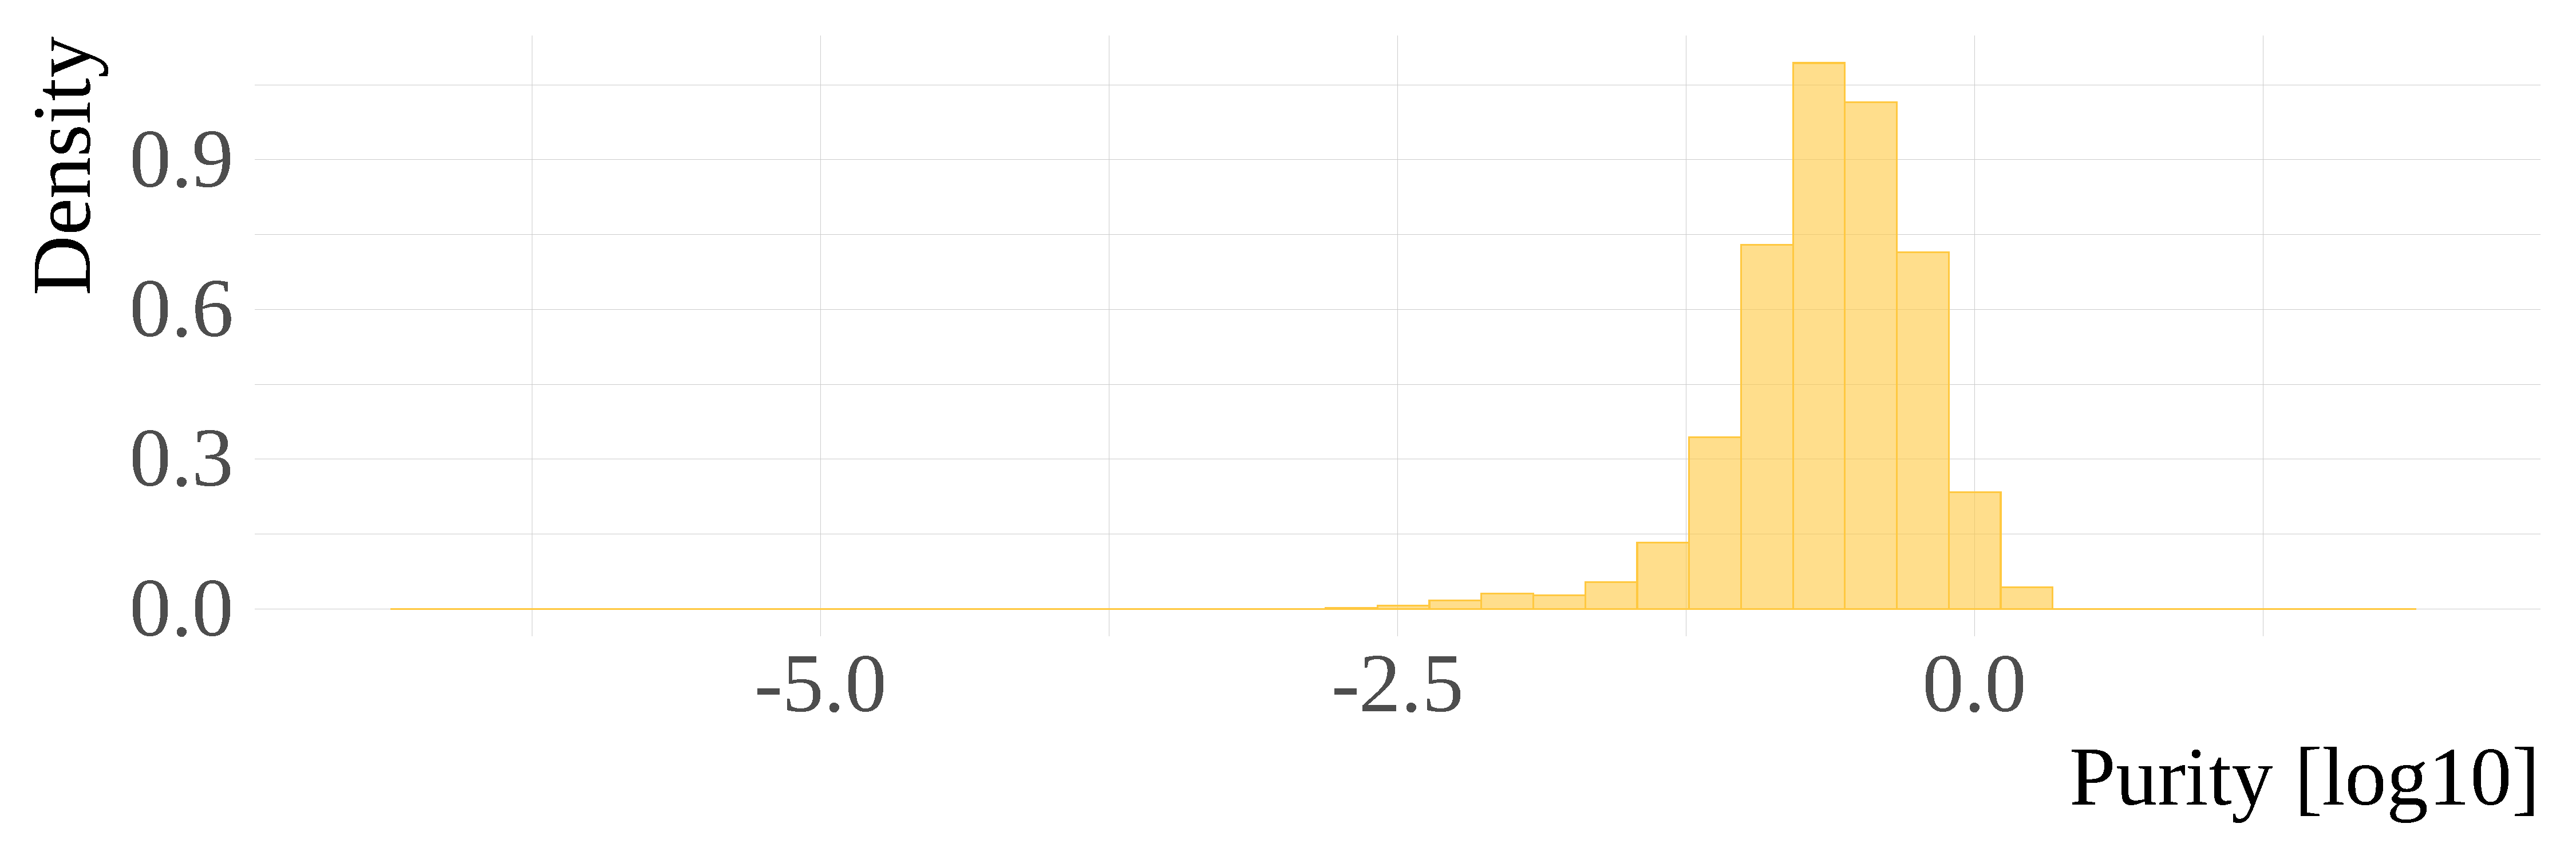
\includegraphics[width = \linewidth]{Figures/Canola_43/log_purity_cn43_5}}
%     \caption{Histograms of the $log10$ of geodesic purity index from Canola 43}
%     \label{fig:histograms_purity_cn43}
% \end{figure}

% \begin{figure}[hbt]
%     \centering
%     \subcaptionbox{16 May 2016}{\includegraphics[width = \linewidth]{Figures/Wheat_104/log_purity_wt104_1}}
%     \subcaptionbox{09 June 2016}{\includegraphics[width = \linewidth]{Figures/Wheat_104/log_purity_wt104_2}}
%     \subcaptionbox{03 July 2016}{\includegraphics[width = \linewidth]{Figures/Wheat_104/log_purity_wt104_3}}
%     \subcaptionbox{27 July 2016}{\includegraphics[width = \linewidth]{Figures/Wheat_104/log_purity_wt104_4}}
%     \subcaptionbox{20 August 2016}{\includegraphics[width = \linewidth]{Figures/Wheat_104/log_purity_wt104_5}}
%     \caption{Histograms of the $log10$ of geodesic purity index from Wheat 104}
%     \label{fig:histograms_purity_wt104}
% \end{figure}

% \begin{figure}[hbt]
%     \centering
%     \subcaptionbox{16 May 2016}{\includegraphics[width = \linewidth]{Figures/Oats_102/log_purity_ot102_1}}
%     \subcaptionbox{09 June 2016}{\includegraphics[width = \linewidth]{Figures/Oats_102/log_purity_ot102_2}}
%     \subcaptionbox{03 July 2016}{\includegraphics[width = \linewidth]{Figures/Oats_102/log_purity_ot102_3}}
%     \subcaptionbox{27 July 2016}{\includegraphics[width = \linewidth]{Figures/Oats_102/log_purity_ot102_4}}
%     \subcaptionbox{20 August 2016}{\includegraphics[width = \linewidth]{Figures/Oats_102/log_purity_ot102_5}}
%     \caption{Histograms of the $log10$ of geodesic purity index from Oats 102}
%     \label{fig:histograms_purity_ot102}
% \end{figure}

%\begin{figure}[hbt]
%  \centering
%  \subcaptionbox{Histograms\label{fig:histograms_purity}}{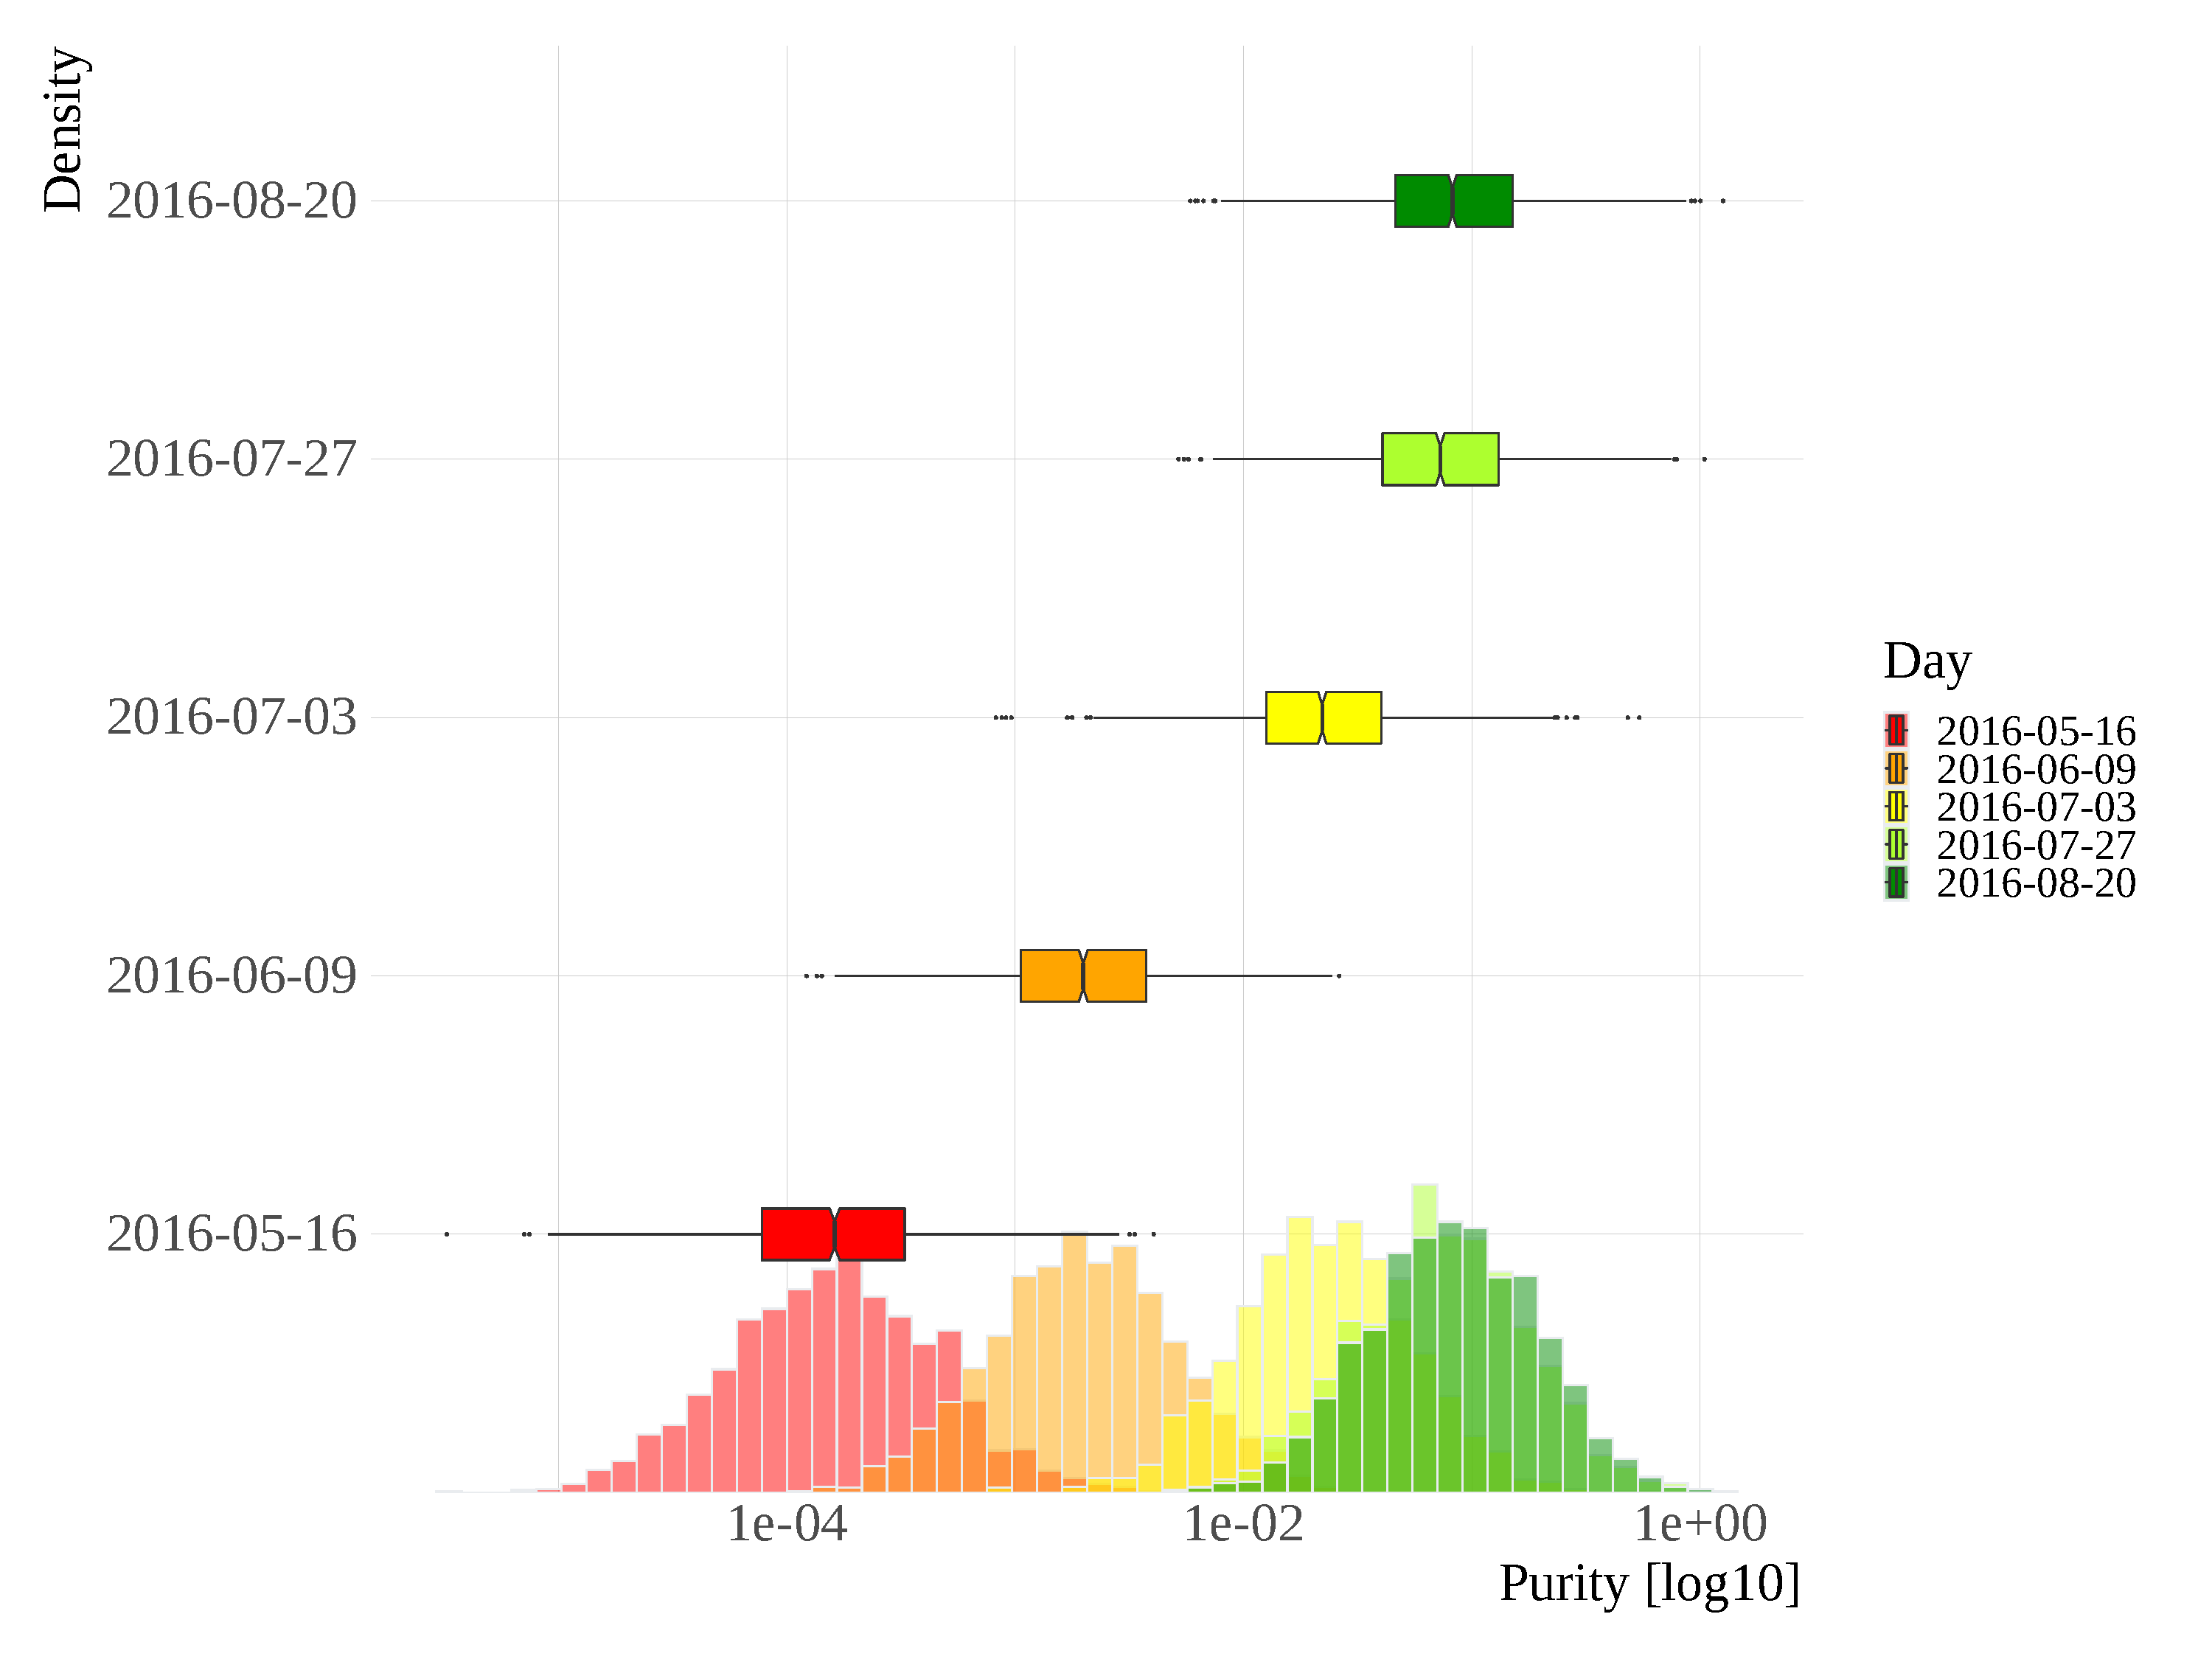
\includegraphics[width = .95\linewidth]{histograms}}
%  \subcaptionbox{QQPlots\label{fig:qqplots}}{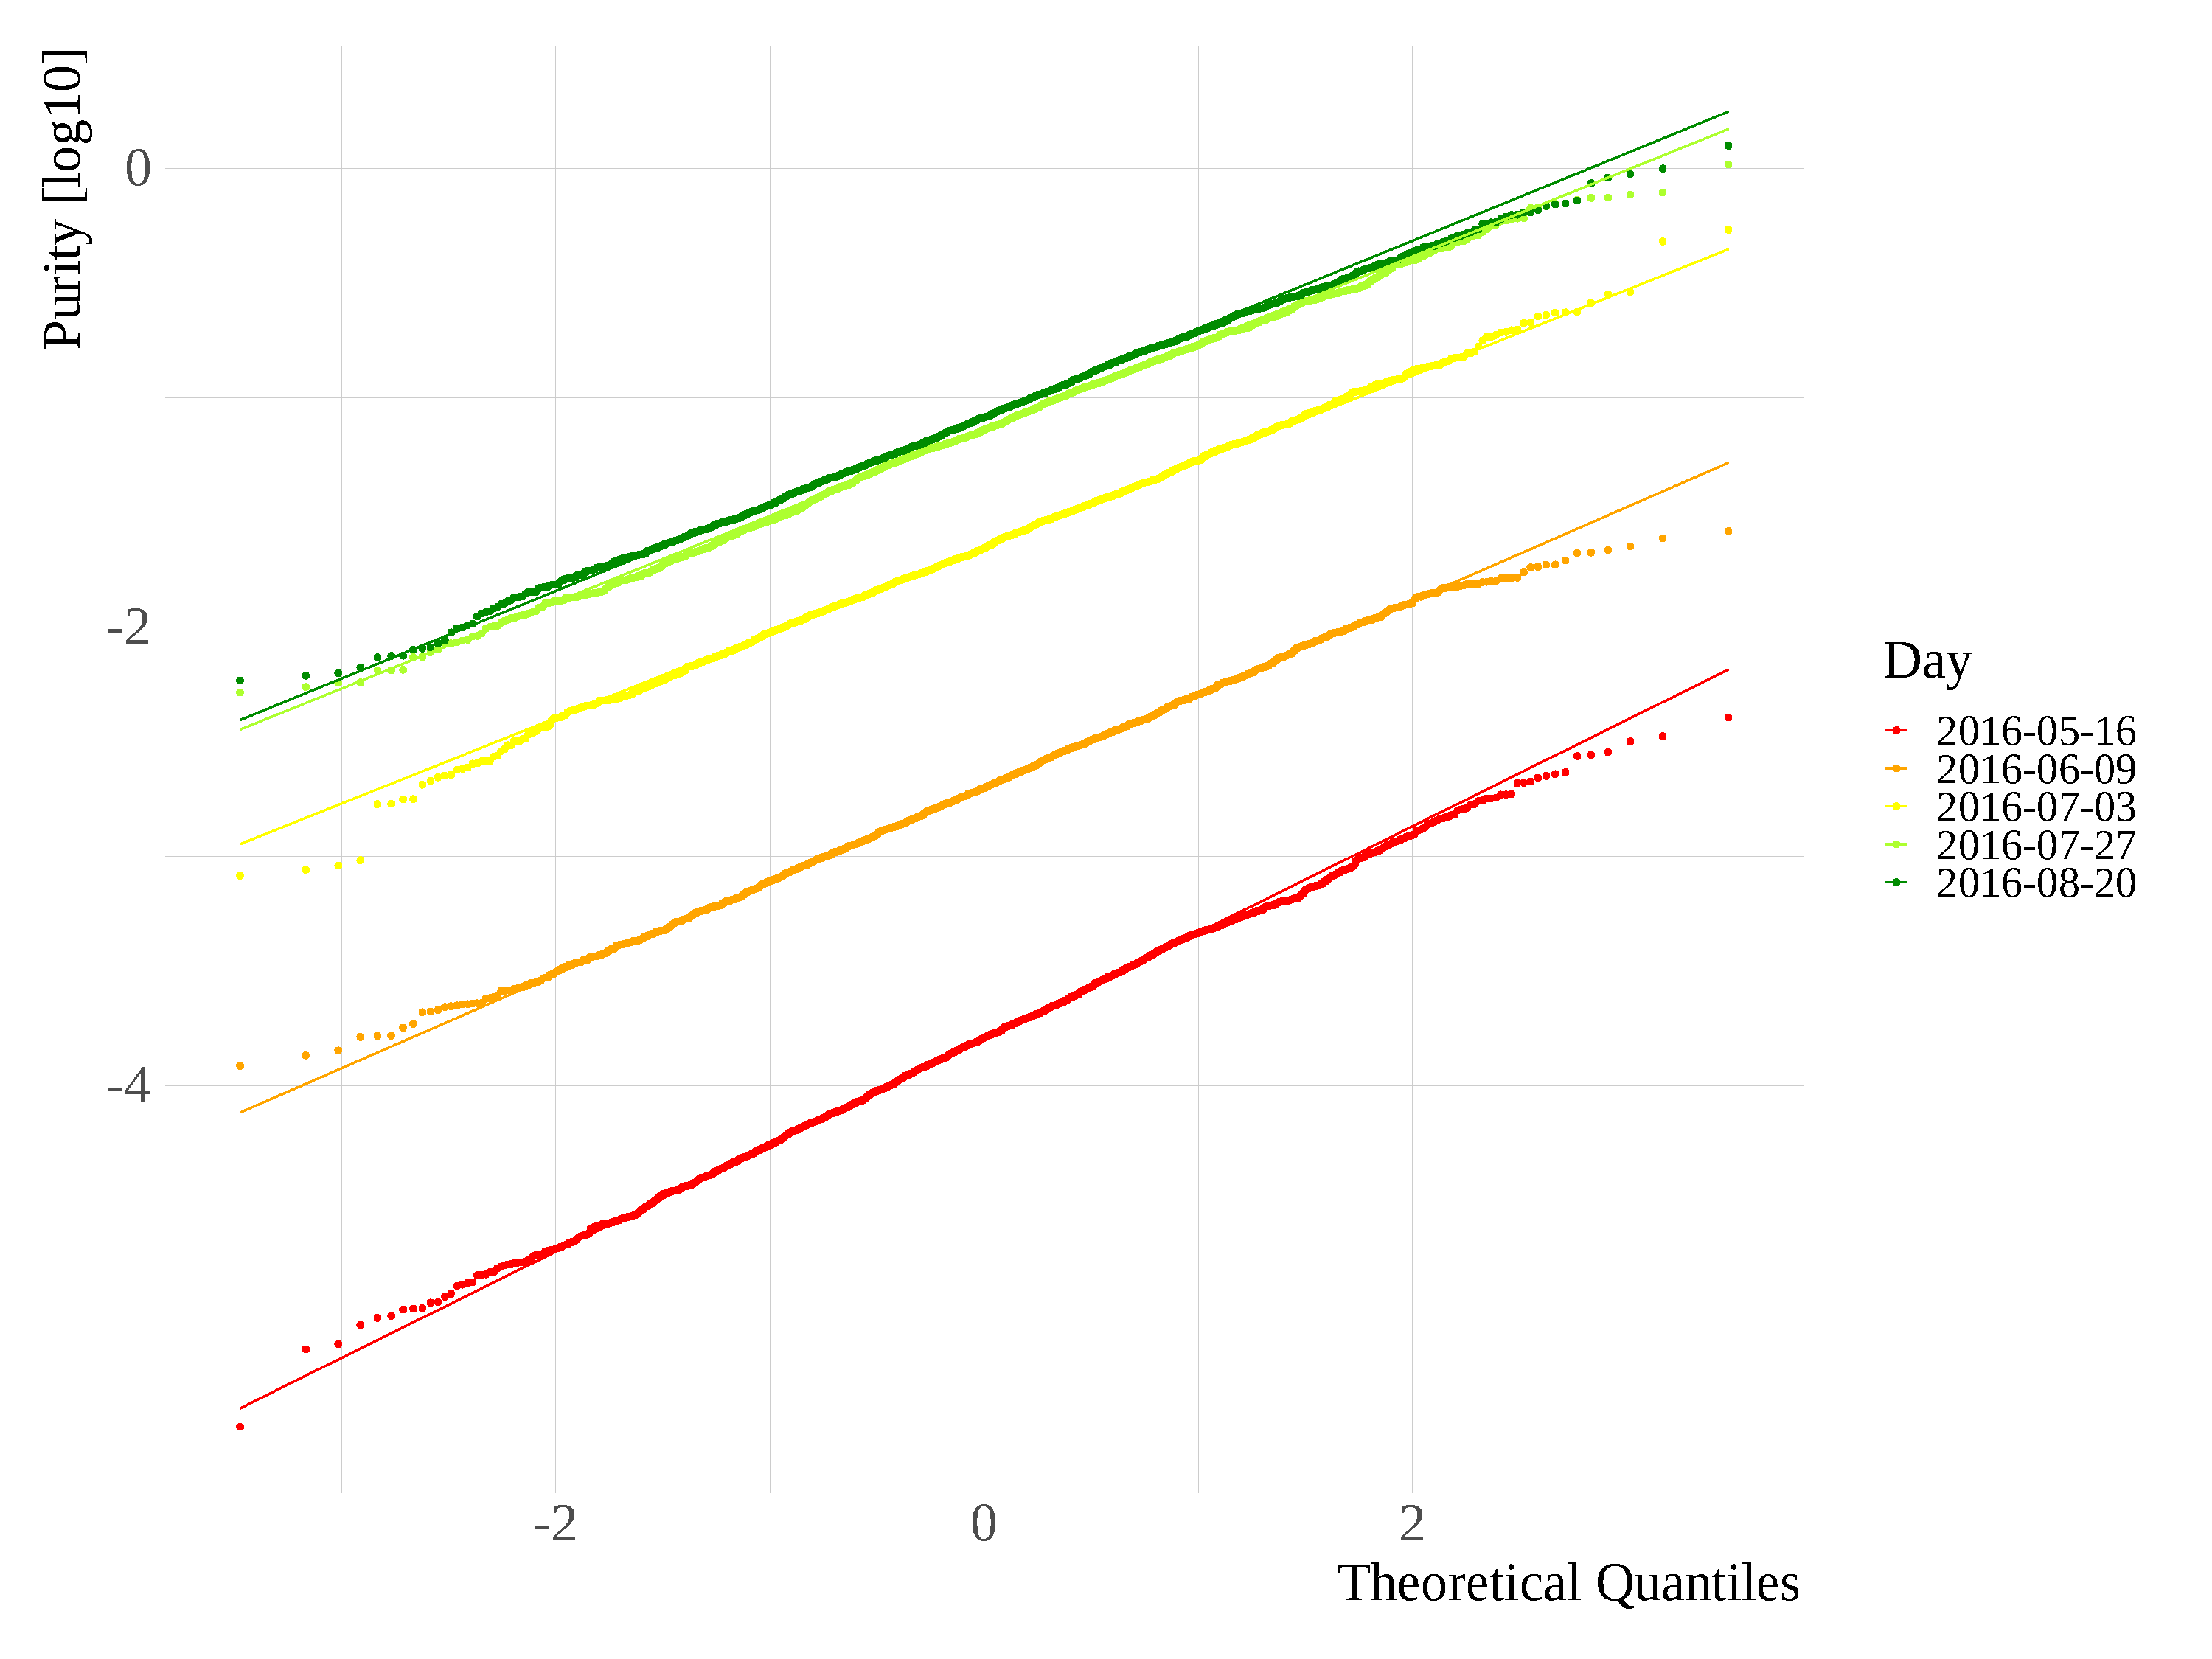
\includegraphics[width = .95\linewidth]{qqplots}}
%  \caption{Descriptive analysis of the logarithm purity values for each image}
%  \label{fig:desc_analysis}
%\end{figure}

% \begin{table}[hbt]
%   \centering
%   \caption{$p$-values from Shapiro-Wilk Test for Soybeans 231}
%   \label{tab:pvalues_purities_sb231}
%   \begin{tabular}{lrrrrr}
%     \toprule
%     \textbf{Day} & \textbf{16 May} & \textbf{09 June} & \textbf{03 July} & \textbf{27 July} & \textbf{20 Aug.}\\
%                  & \textbf{2016} & \textbf{2016} & \textbf{2016} & \textbf{2016} & \textbf{2016}\\\midrule

%     \textbf{$p$-value} & 0.4963 & 0.0650 & 0.3494 & 0.0585 & 0.3919\\
%     \bottomrule
%   \end{tabular}
% \end{table}

% \begin{table}[hbt]
%   \centering
%   \caption{$p$-values from Shapiro-Wilk Test for Canola 43}
%   \label{tab:pvalues_purities_sb231}
%   \begin{tabular}{lrrrrr}
%     \toprule
%     \textbf{Day} & \textbf{16 May} & \textbf{09 June} & \textbf{03 July} & \textbf{27 July} & \textbf{20 Aug.}\\
%                  & \textbf{2016} & \textbf{2016} & \textbf{2016} & \textbf{2016} & \textbf{2016}\\\midrule

%     \textbf{$p$-value} & 0.1143 & 0.7359 & 0.5855 & $2.6\times 10^{-16}$ & $2.6\times 10^{-16}$\\
%     \bottomrule
%   \end{tabular}
% \end{table}

% \begin{table}[hbt]
%   \centering
%   \caption{$p$-values from Shapiro-Wilk Test for Wheat 104}
%   \label{tab:pvalues_purities_sb231}
%   \begin{tabular}{lrrrrr}
%     \toprule
%     \textbf{Day} & \textbf{16 May} & \textbf{09 June} & \textbf{03 July} & \textbf{27 July} & \textbf{20 Aug.}\\
%                  & \textbf{2016} & \textbf{2016} & \textbf{2016} & \textbf{2016} & \textbf{2016}\\\midrule

%     \textbf{$p$-value} & 0.8189 & 0.9042 & 0.0025 & 0.3929 & 0.0544\\
%     \bottomrule
%   \end{tabular}
% \end{table}

% \begin{table}[hbt]
%   \centering
%   \caption{$p$-values from Shapiro-Wilk Test for Oats 102}
%   \label{tab:pvalues_purities_sb231}
%   \begin{tabular}{lrrrrr}
%     \toprule
%     \textbf{Day} & \textbf{16 May} & \textbf{09 June} & \textbf{03 July} & \textbf{27 July} & \textbf{20 Aug.}\\
%                  & \textbf{2016} & \textbf{2016} & \textbf{2016} & \textbf{2016} & \textbf{2016}\\\midrule

%     \textbf{$p$-value} & 0.4928 & $5.24\times 10^{-8}$ & 0.5263 & 0.0484 & 0.9694\\
%     \bottomrule
%   \end{tabular}
% \end{table}


%\section{Data analysis}


%\begin{figure}[hbt]
%\centering
%\subcaptionbox{16 May 2016}{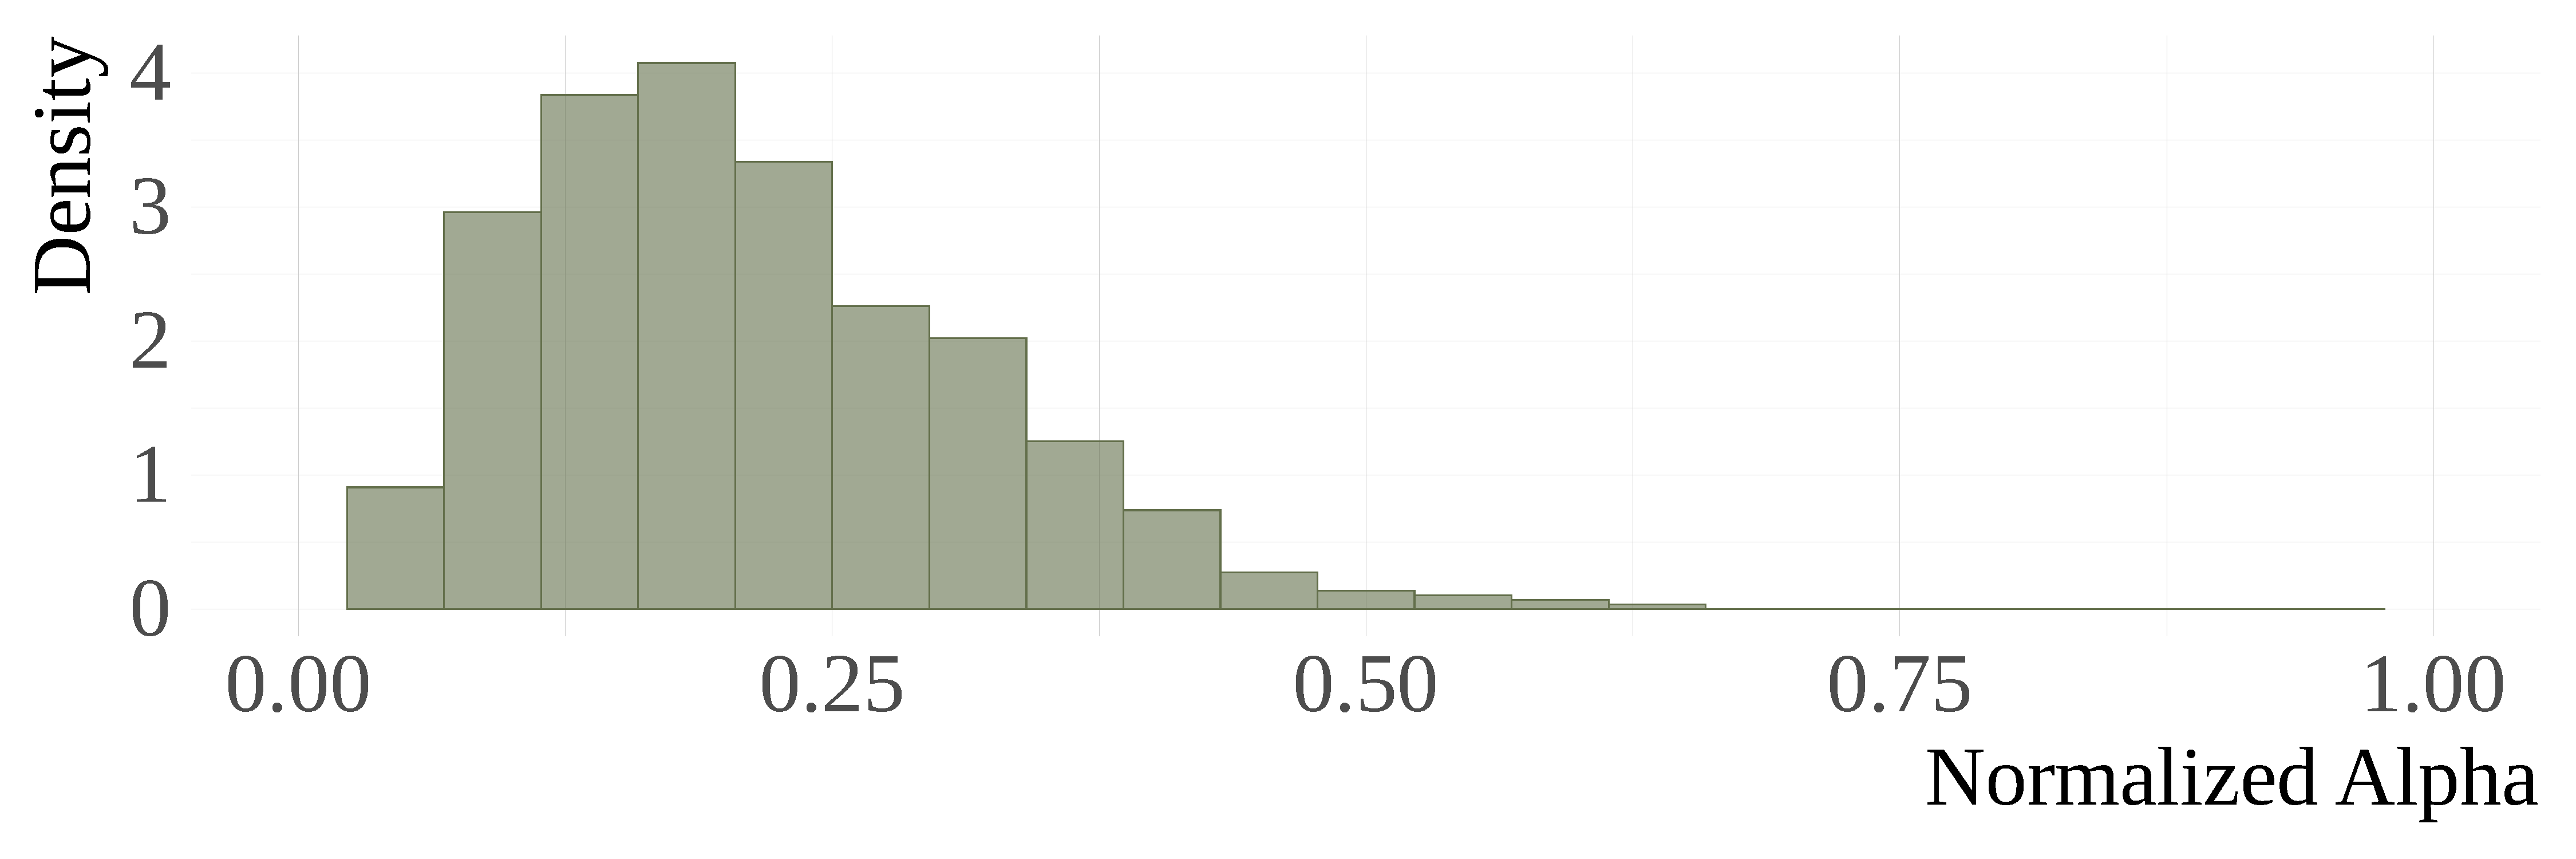
\includegraphics[width = \linewidth]{alpha_sb231_1}}
%\subcaptionbox{09 June 2016}{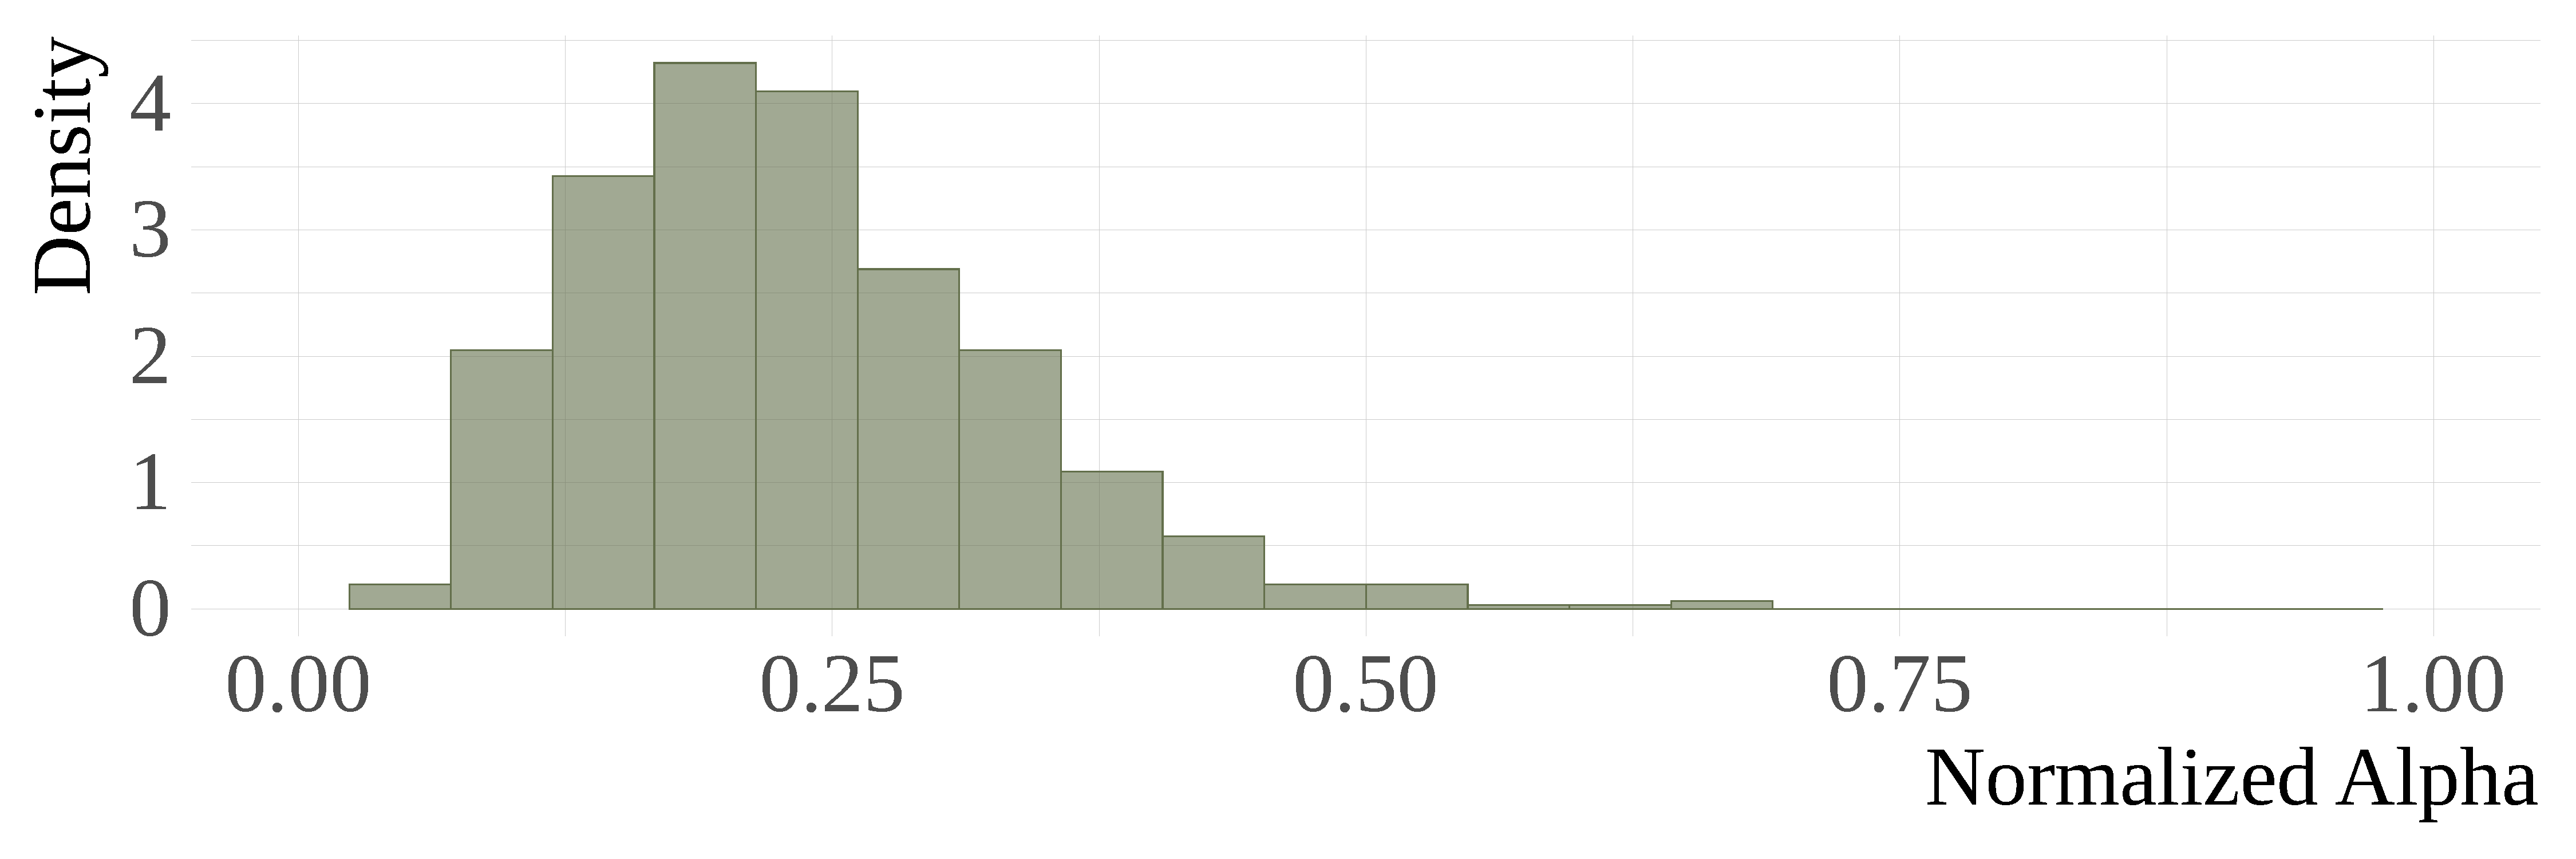
\includegraphics[width = \linewidth]{alpha_sb231_2}}
%\subcaptionbox{03 July 2016}{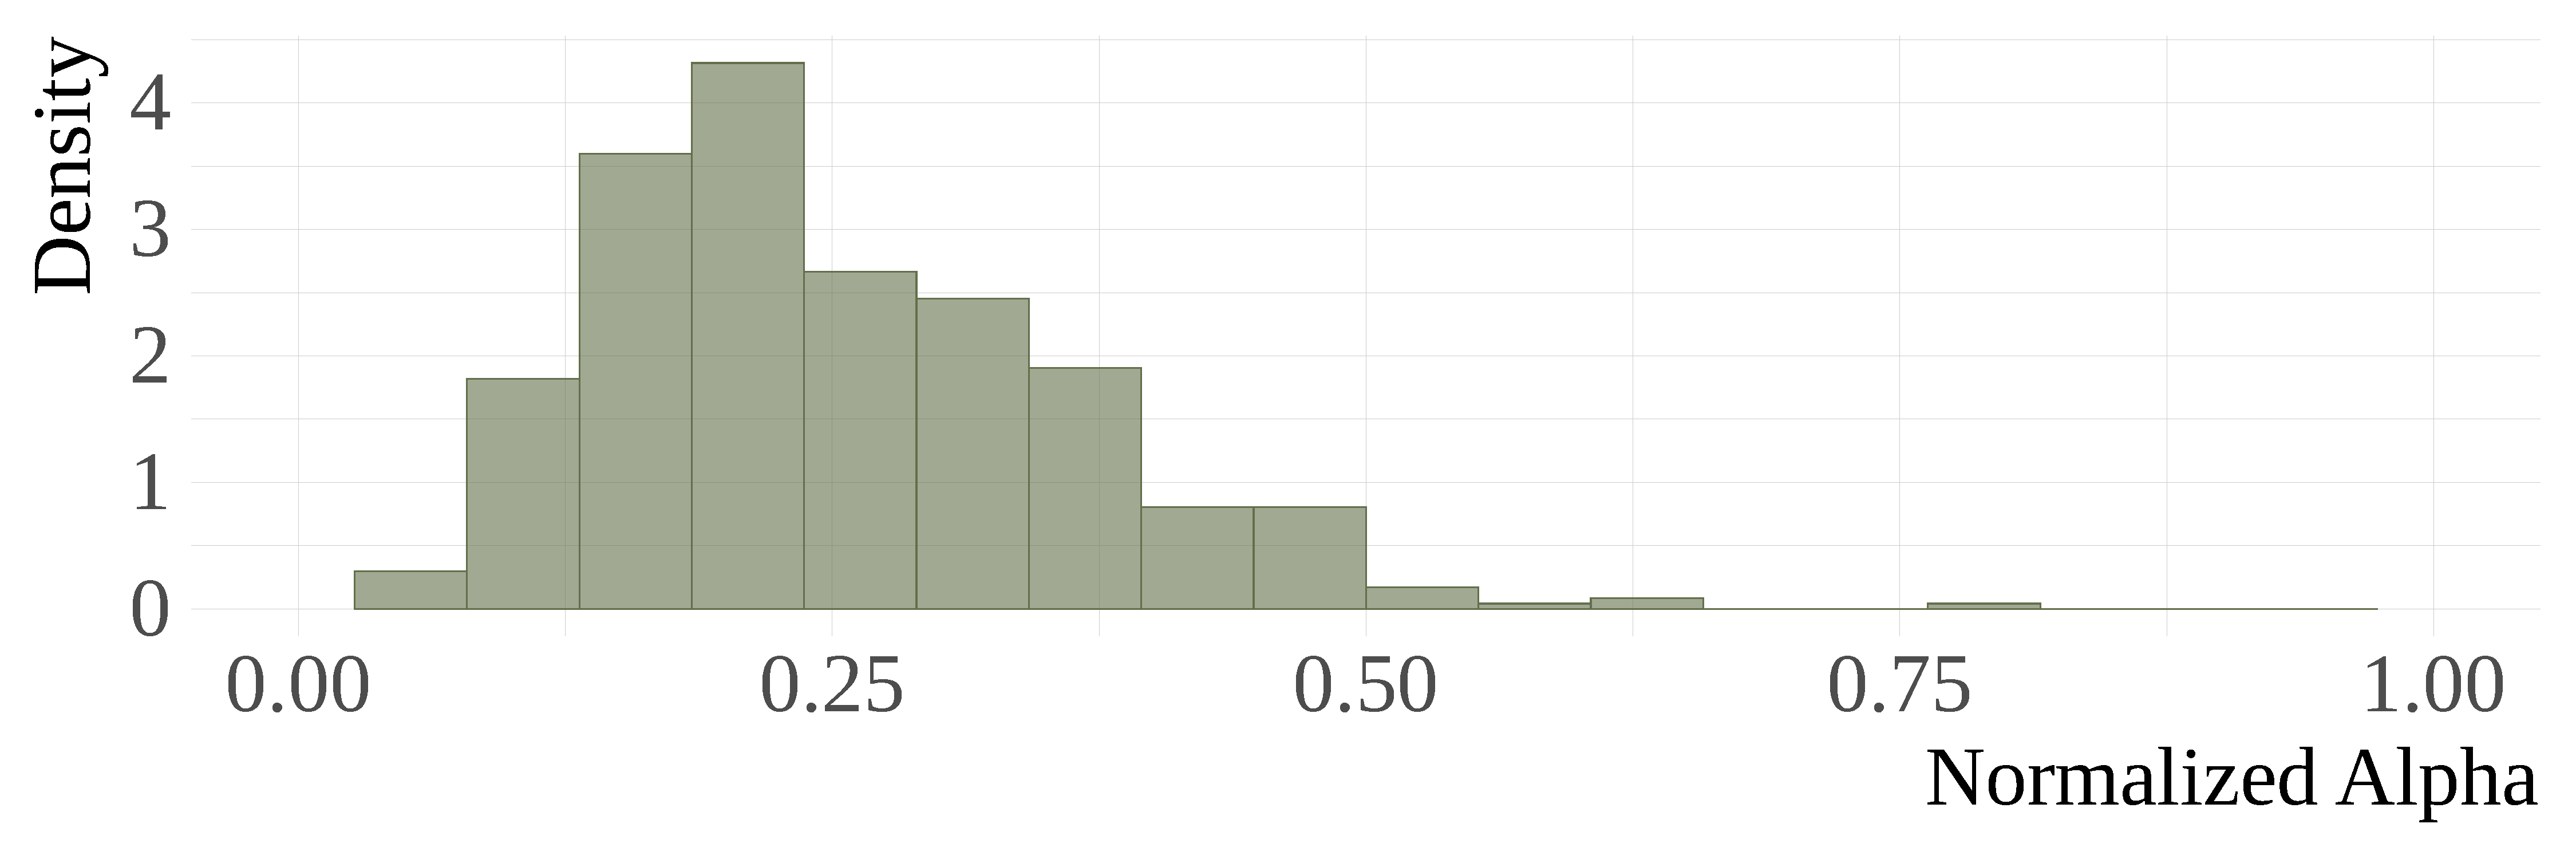
\includegraphics[width = \linewidth]{alpha_sb231_3}}
%\subcaptionbox{27 July 2016}{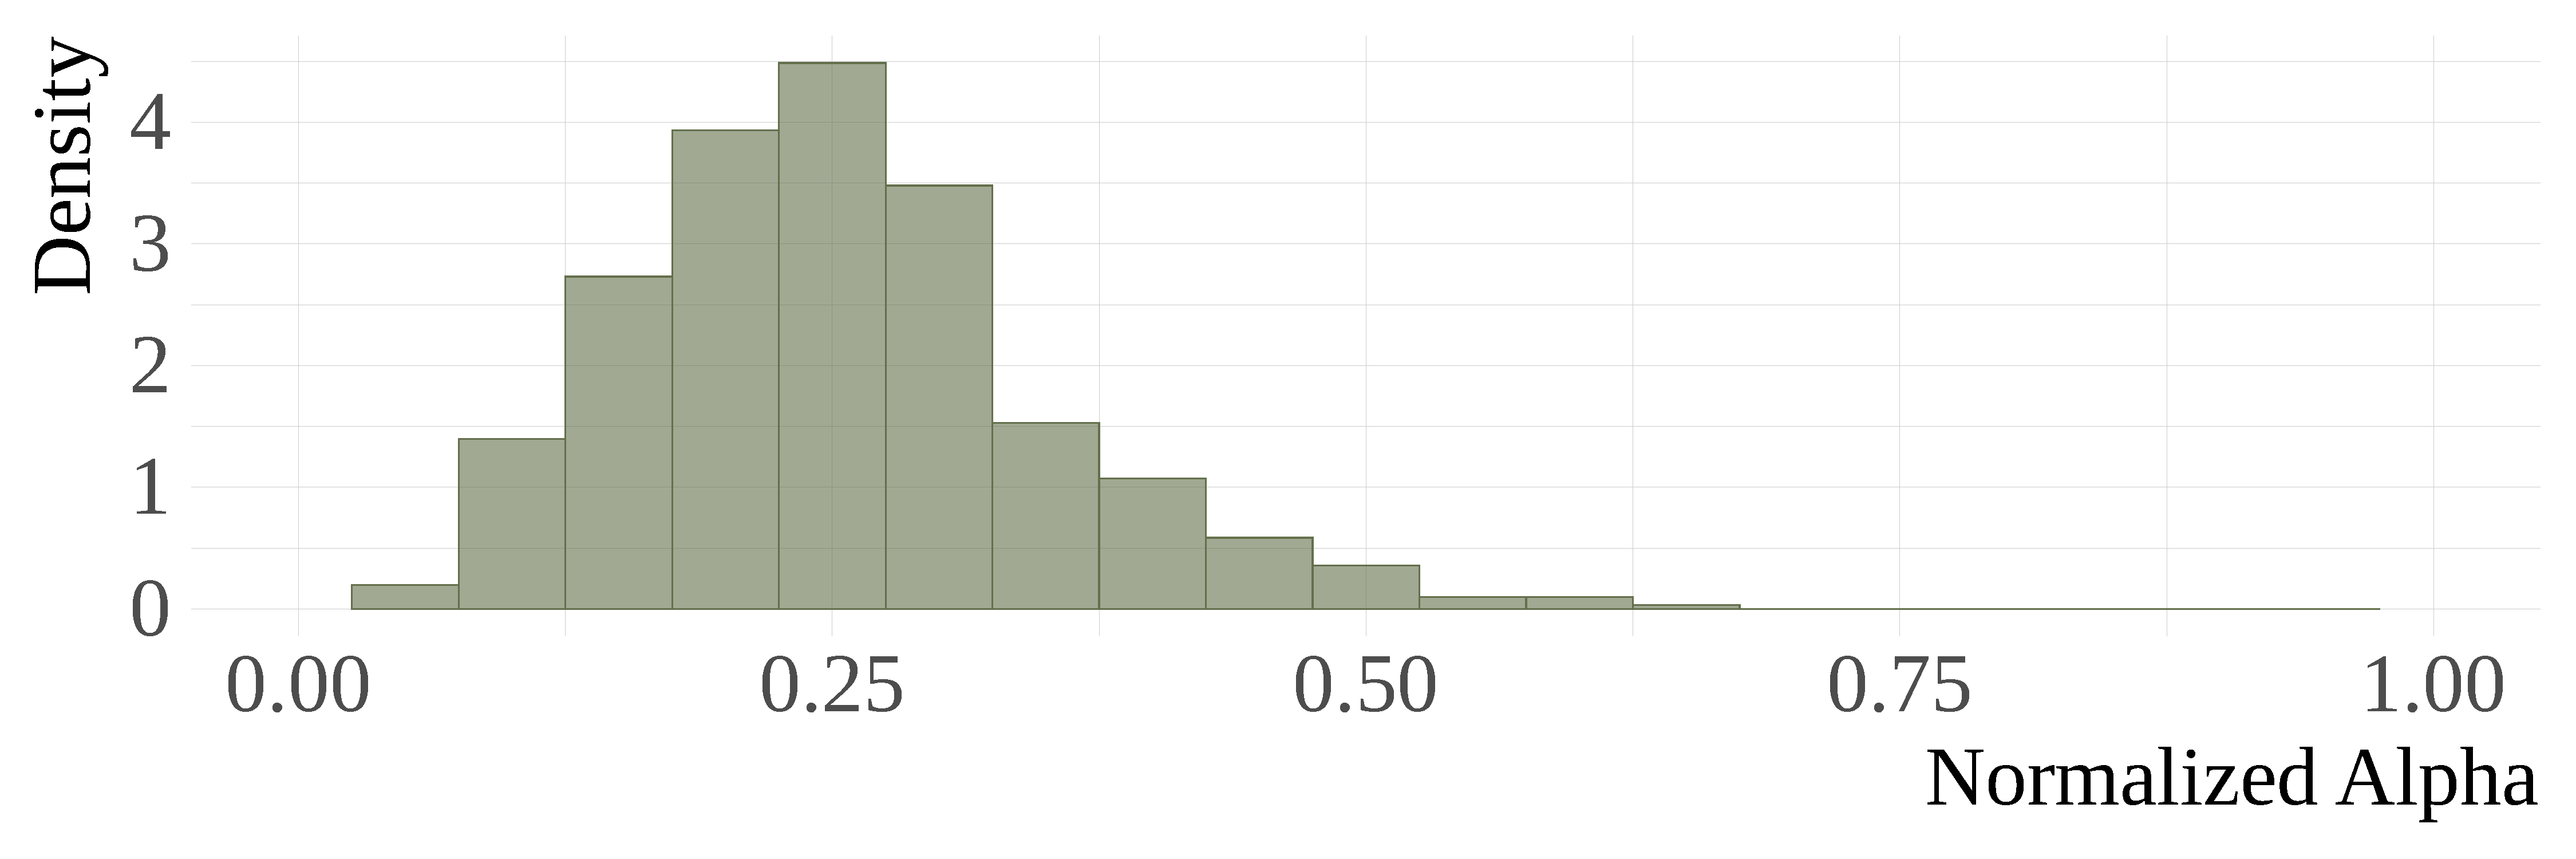
\includegraphics[width = \linewidth]{alpha_sb231_4}}
%\subcaptionbox{20 August 2016}{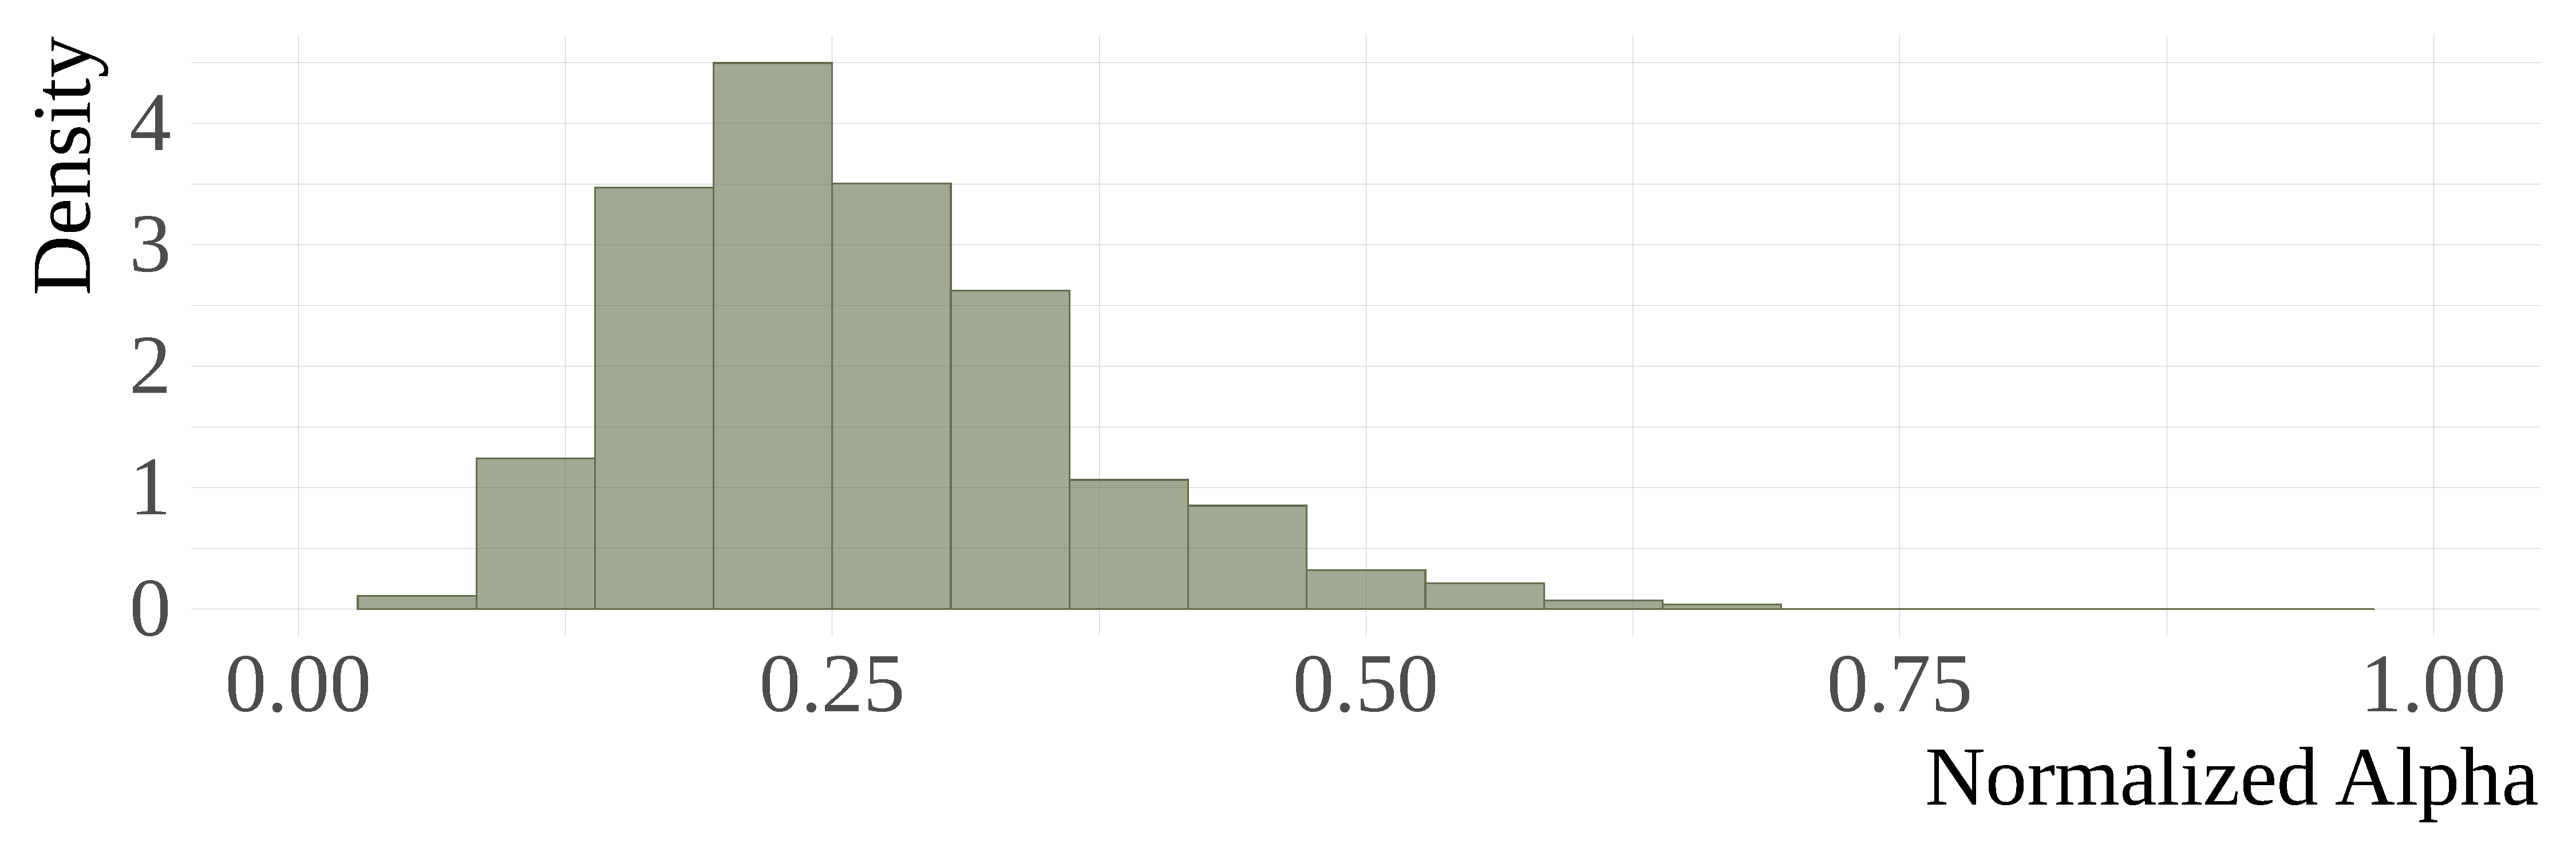
\includegraphics[width = \linewidth]{alpha_sb231_5}}
%\caption{Histograms of the geodesic distances between trihedral and the pixels from Soybeans 231 most similar to trihedral}
%\label{fig:histograms_alpha_sb231}
%\end{figure}

%\begin{figure}[hbt]
%\centering
%\subcaptionbox{16 May 2016}{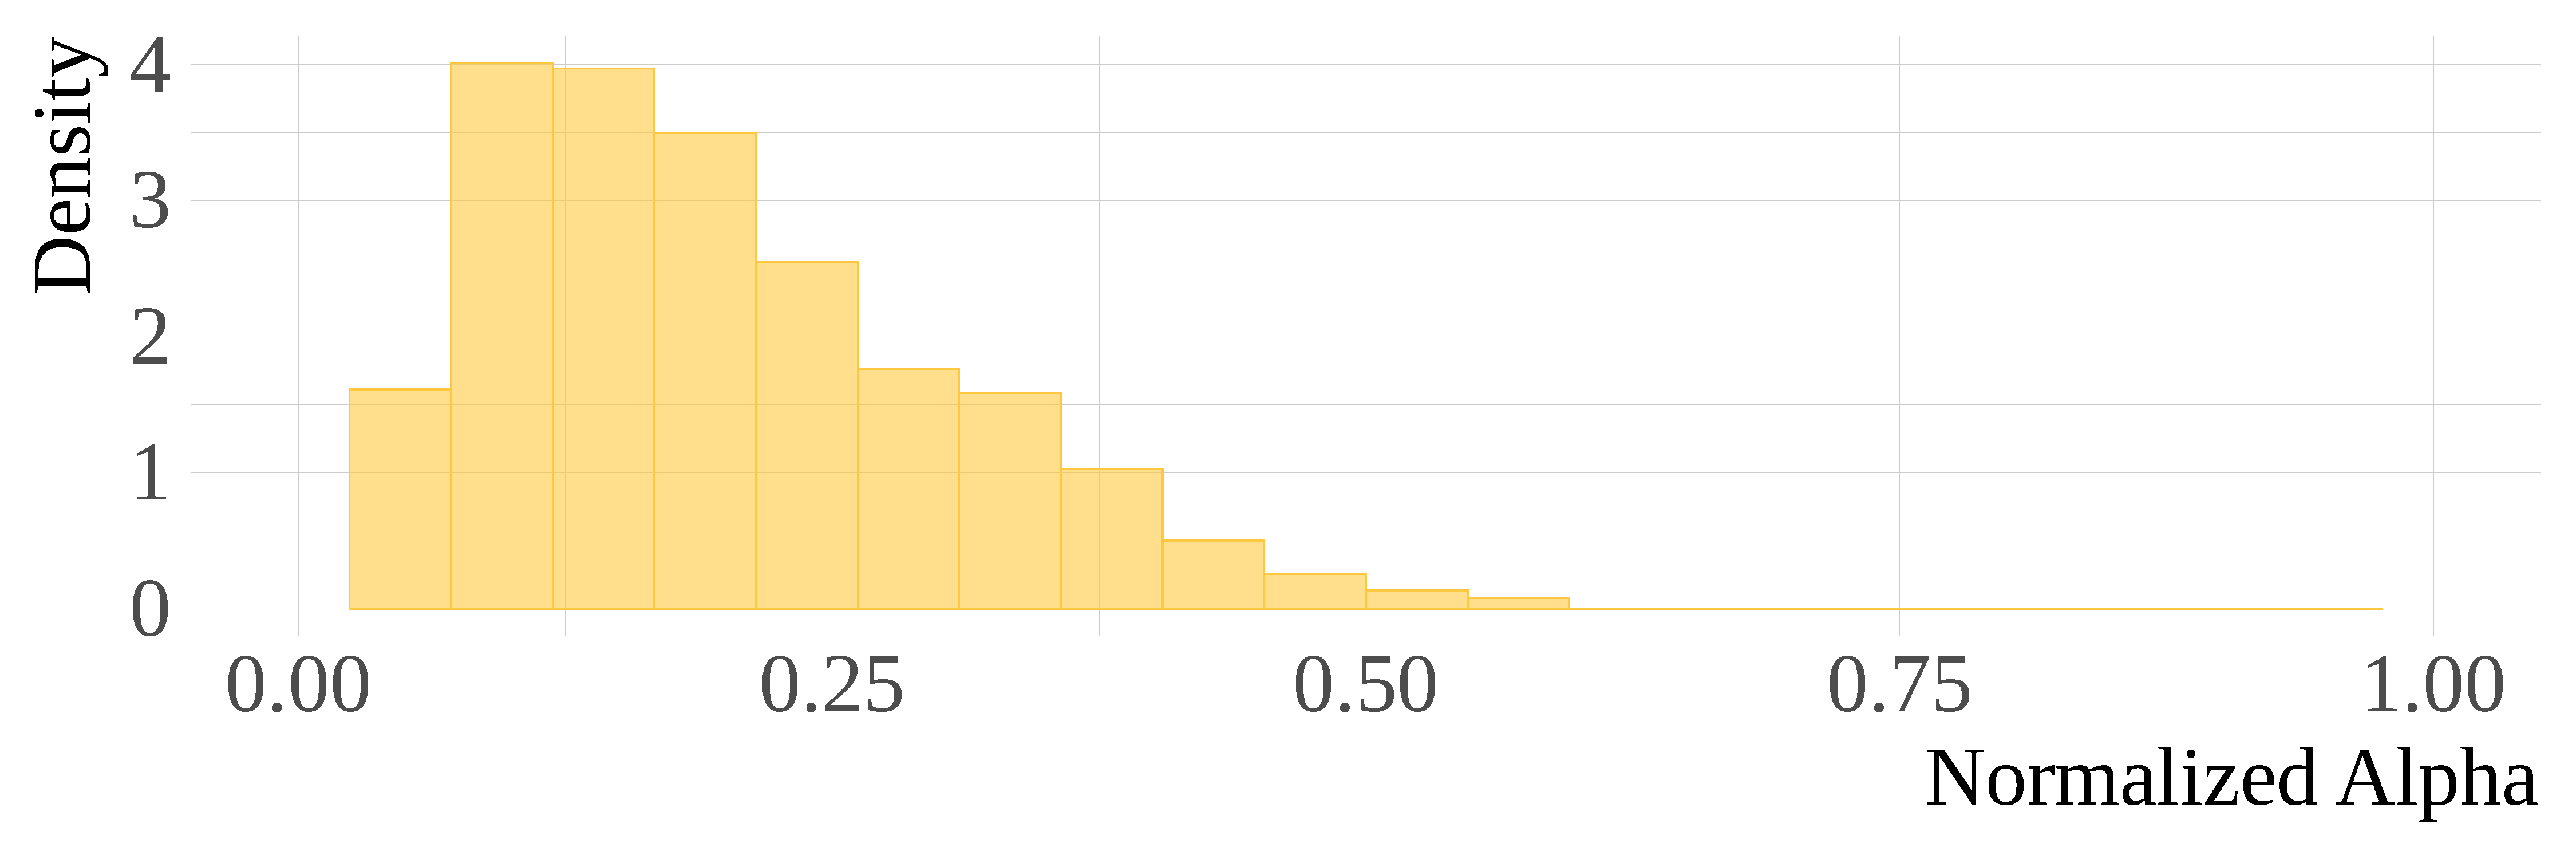
\includegraphics[width = \linewidth]{alpha_cn43_1}}
%\subcaptionbox{09 June 2016}{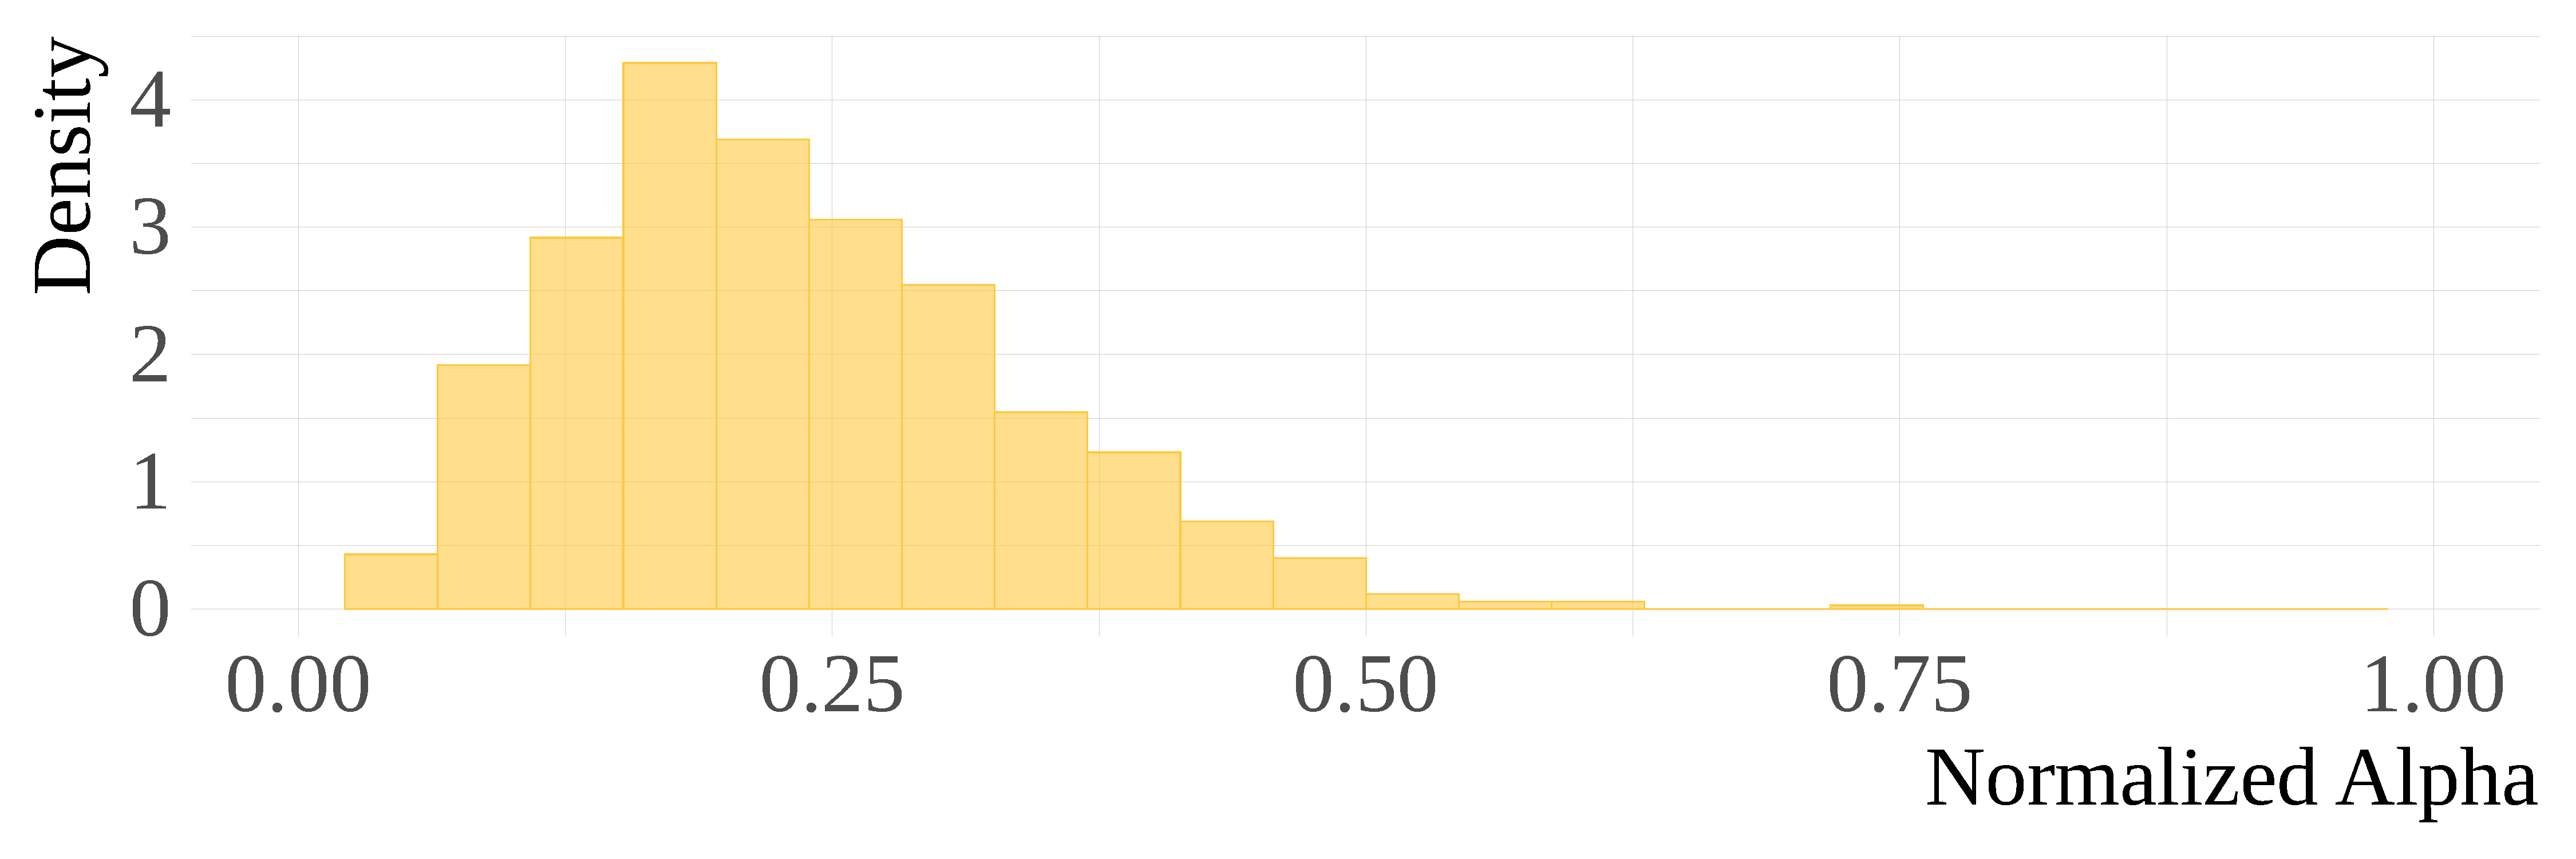
\includegraphics[width = \linewidth]{alpha_cn43_2}}
%\subcaptionbox{03 July 2016}{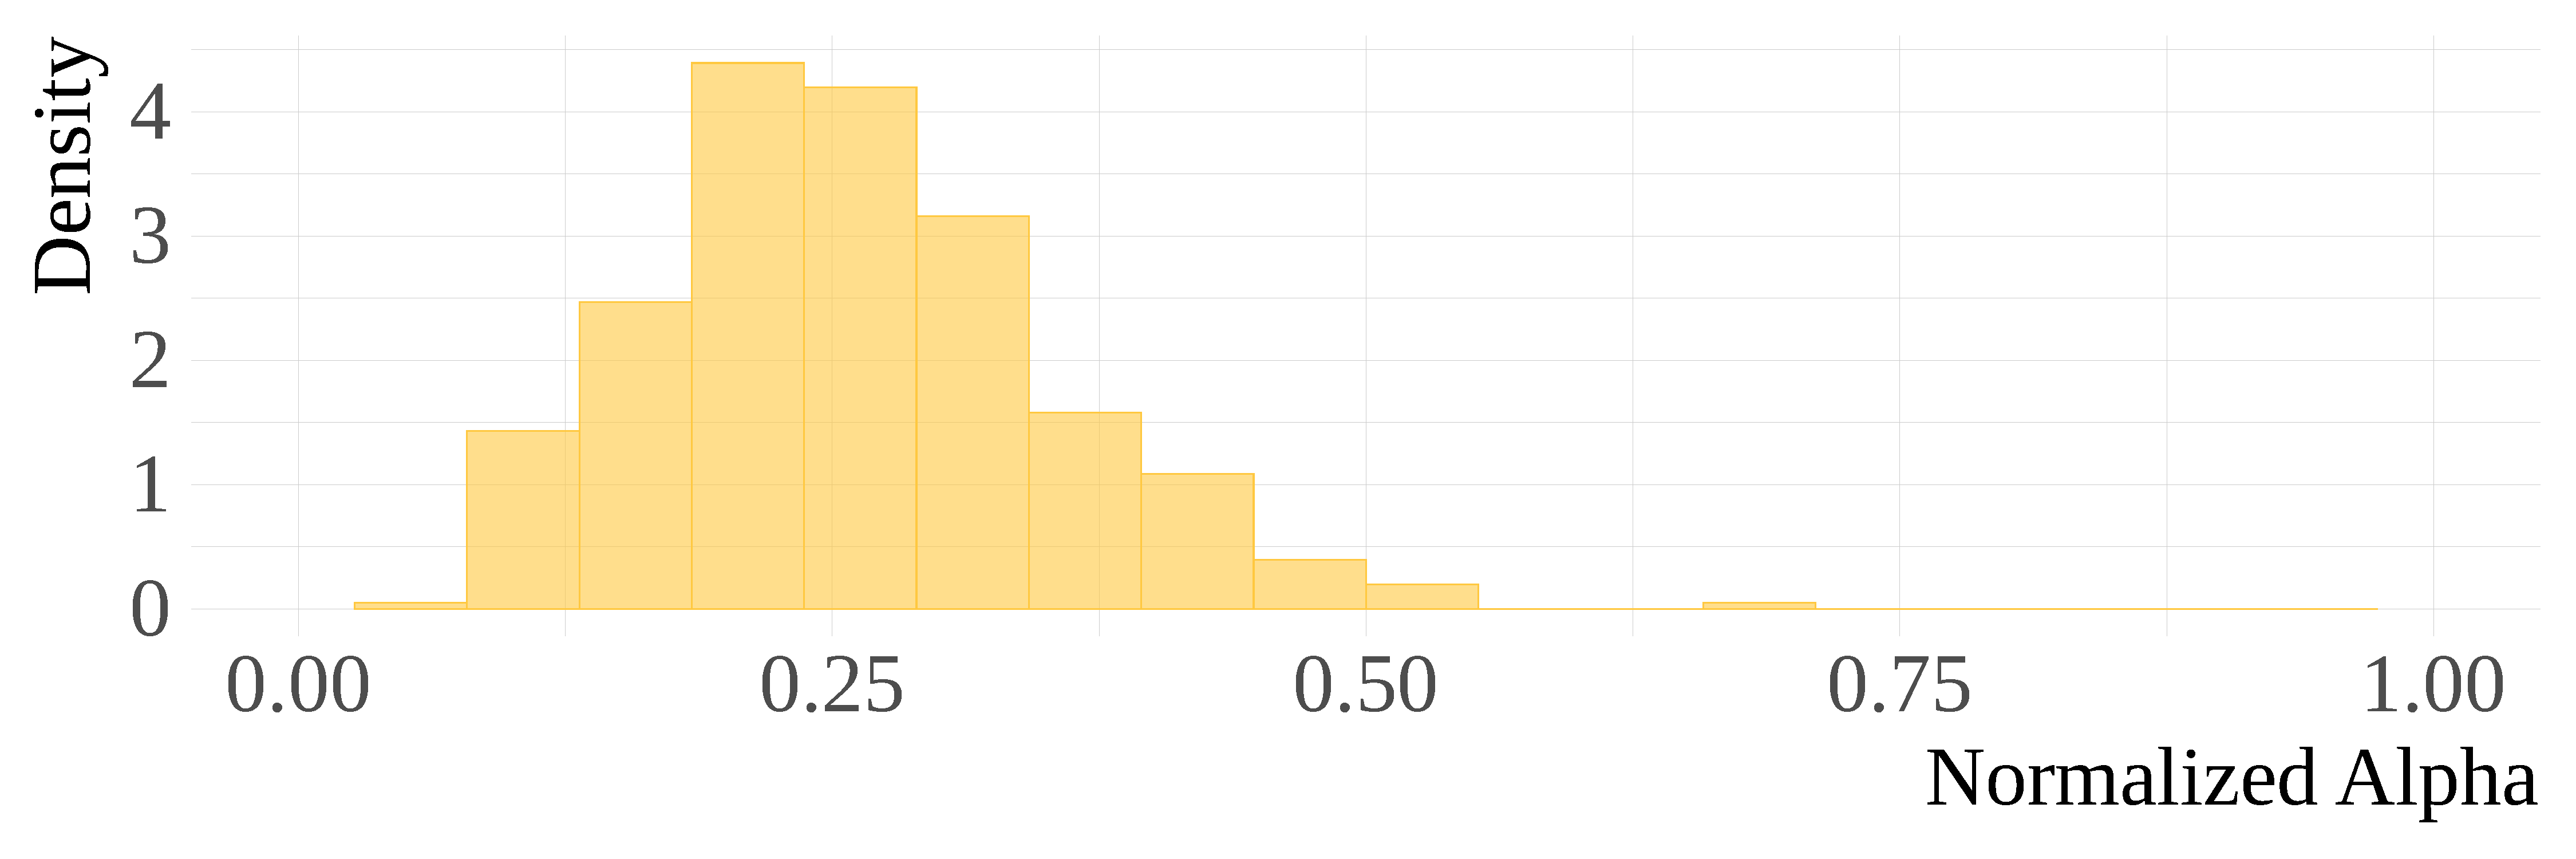
\includegraphics[width = \linewidth]{alpha_cn43_3}}
%\subcaptionbox{27 July 2016}{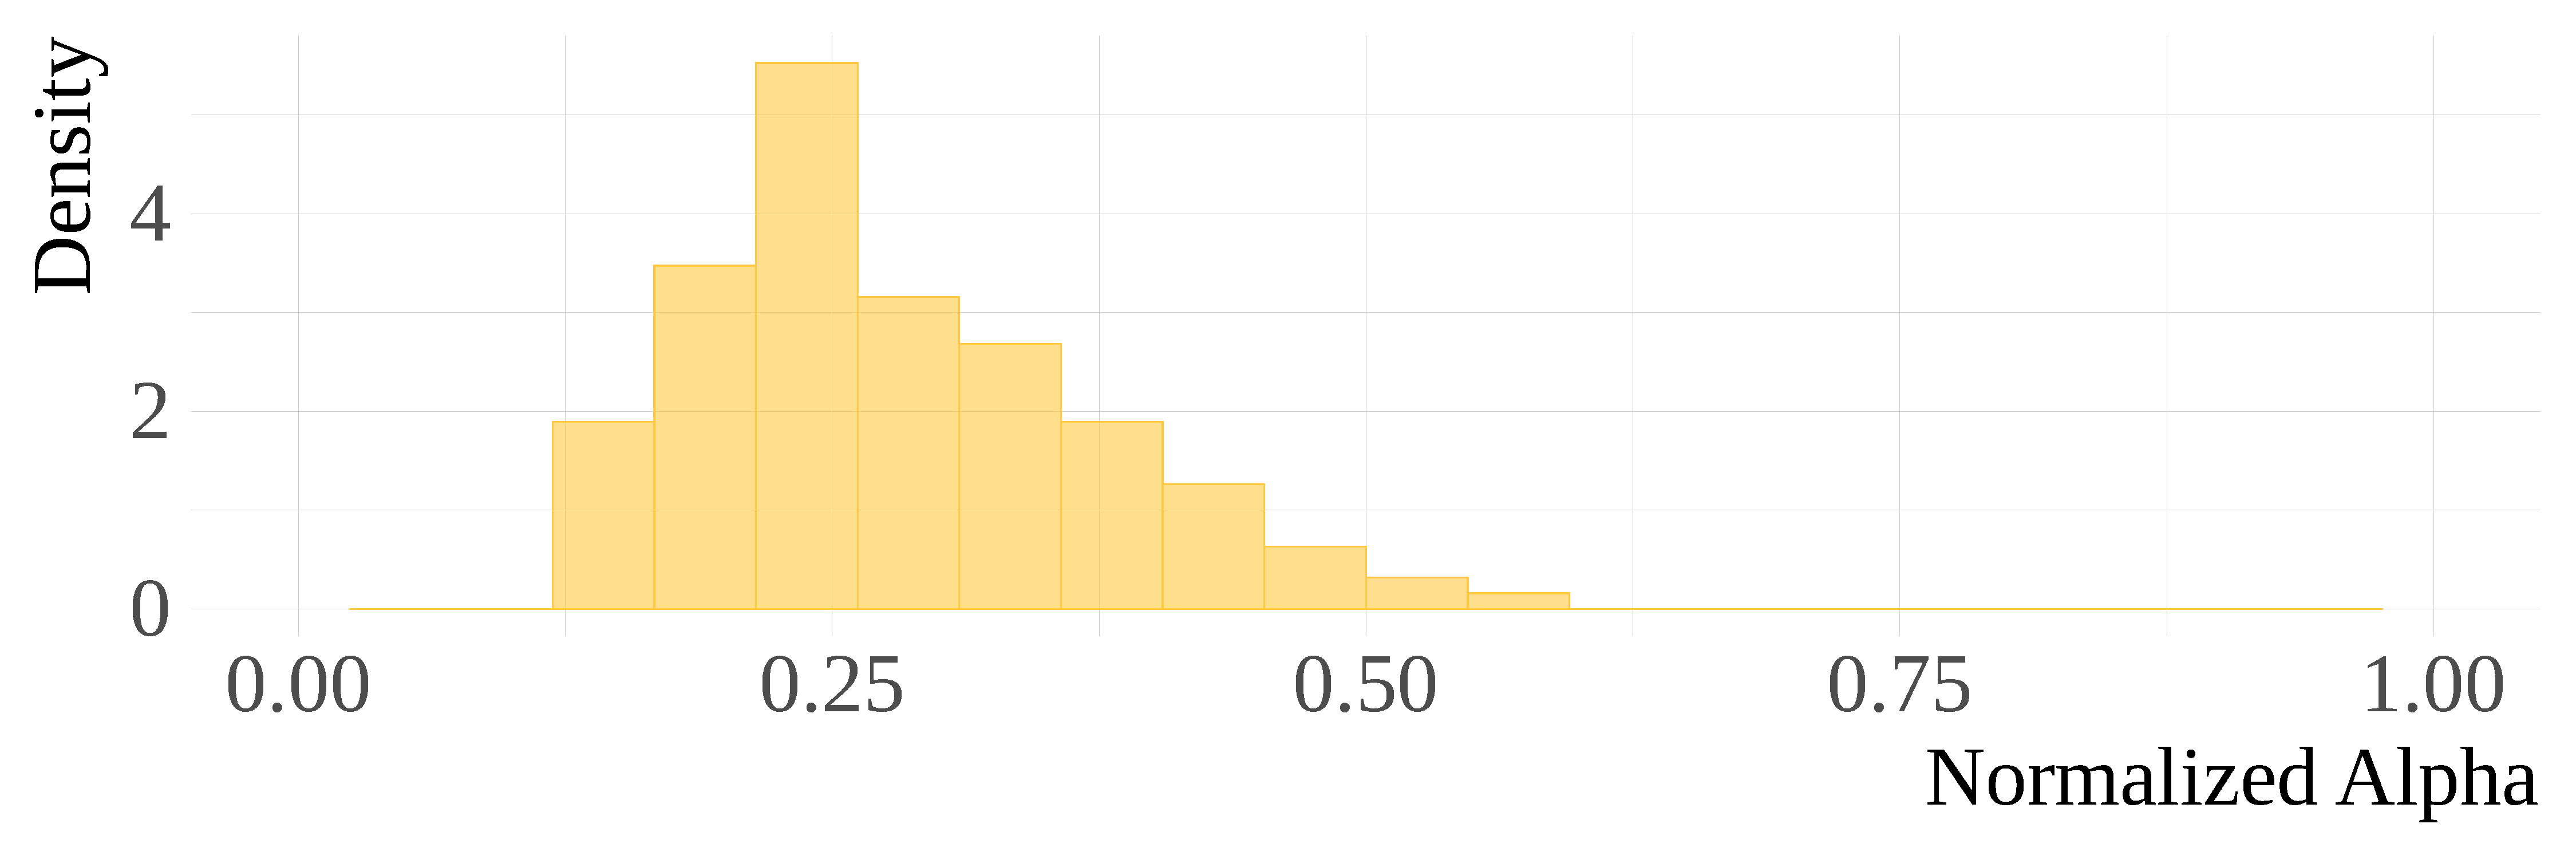
\includegraphics[width = \linewidth]{alpha_cn43_4}}
%\subcaptionbox{20 August 2016}{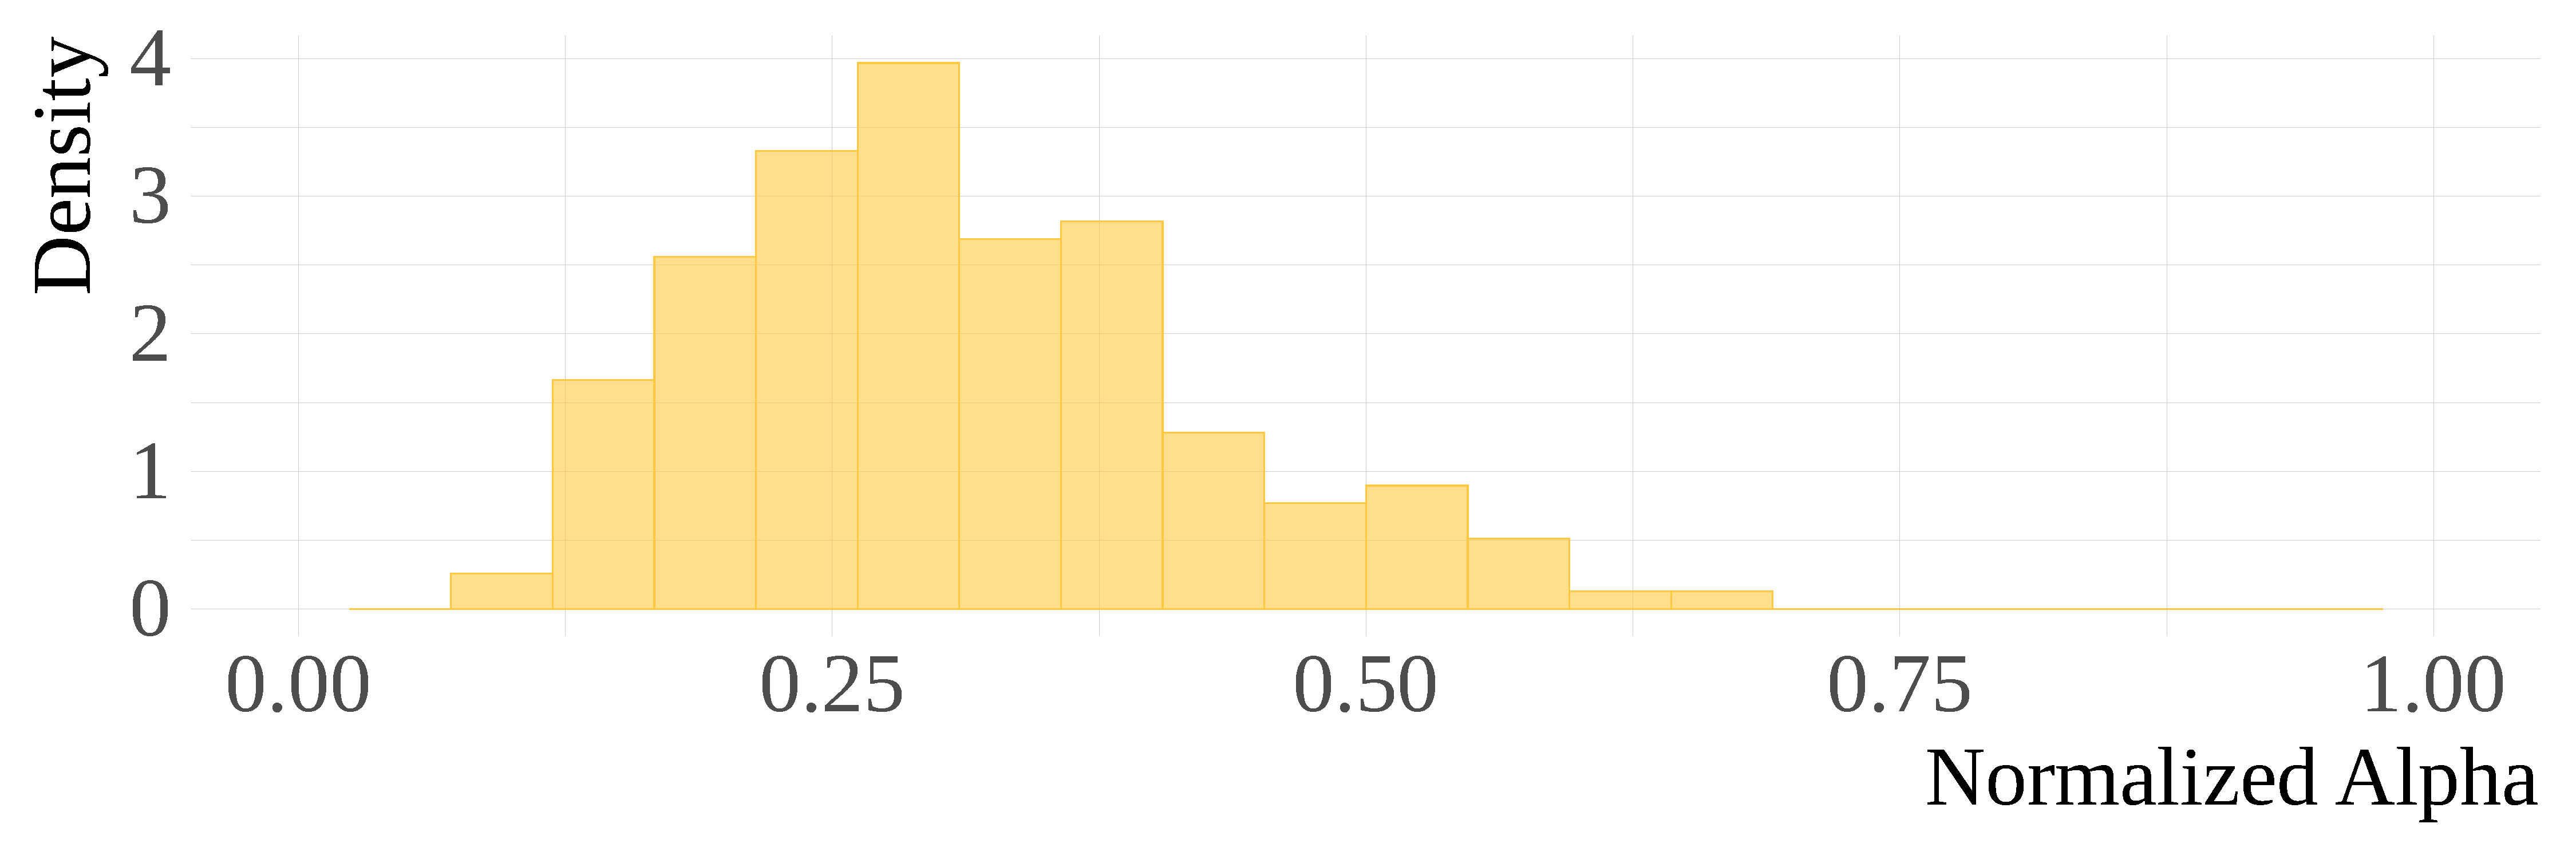
\includegraphics[width = \linewidth]{alpha_cn43_5}}
%\caption{Histograms of the geodesic distances between trihedral and the pixels from Canola 43 most similar to trihedral}
%\label{fig:histograms_alpha_cn43}
%\end{figure}

%\begin{figure}[hbt]
%\centering
%\subcaptionbox{16 May 2016}{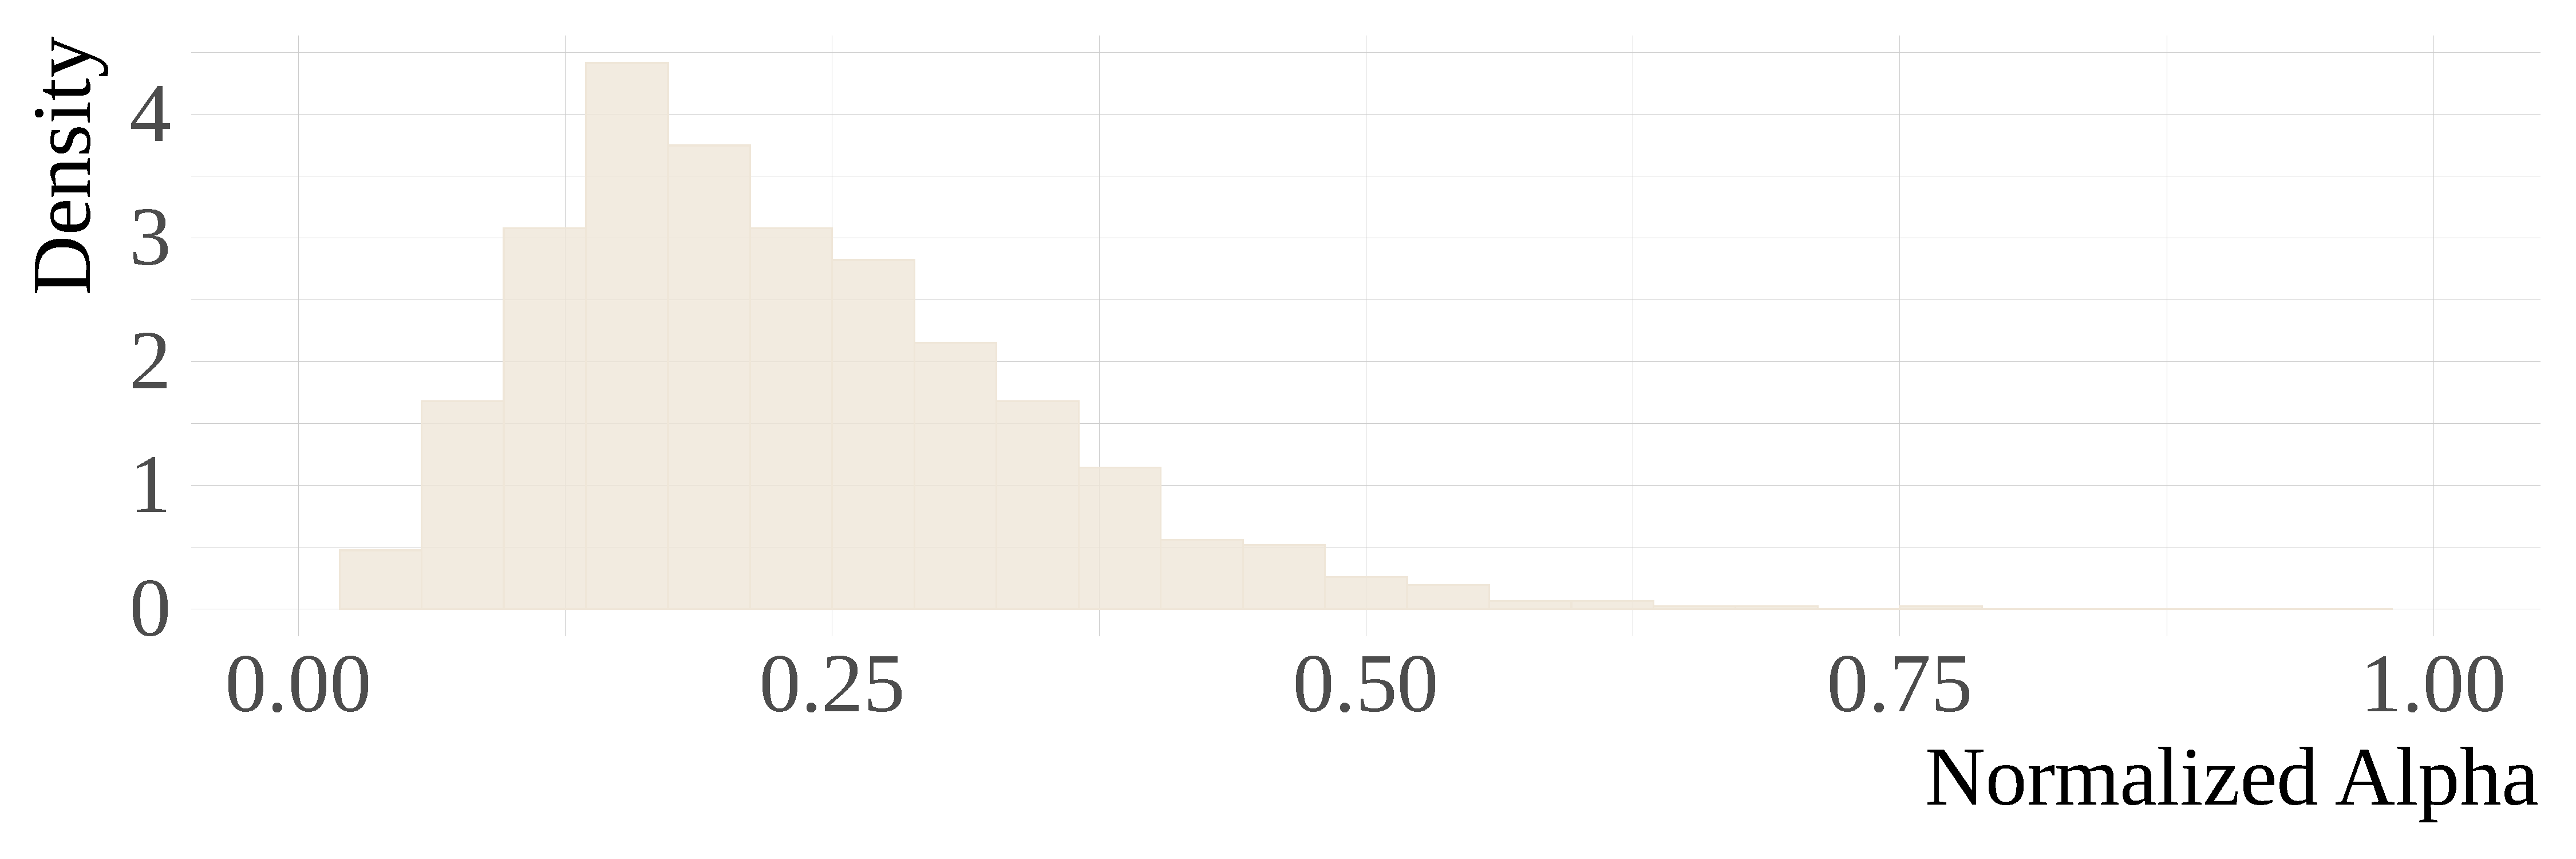
\includegraphics[width = \linewidth]{alpha_ot102_1}}
%\subcaptionbox{09 June 2016}{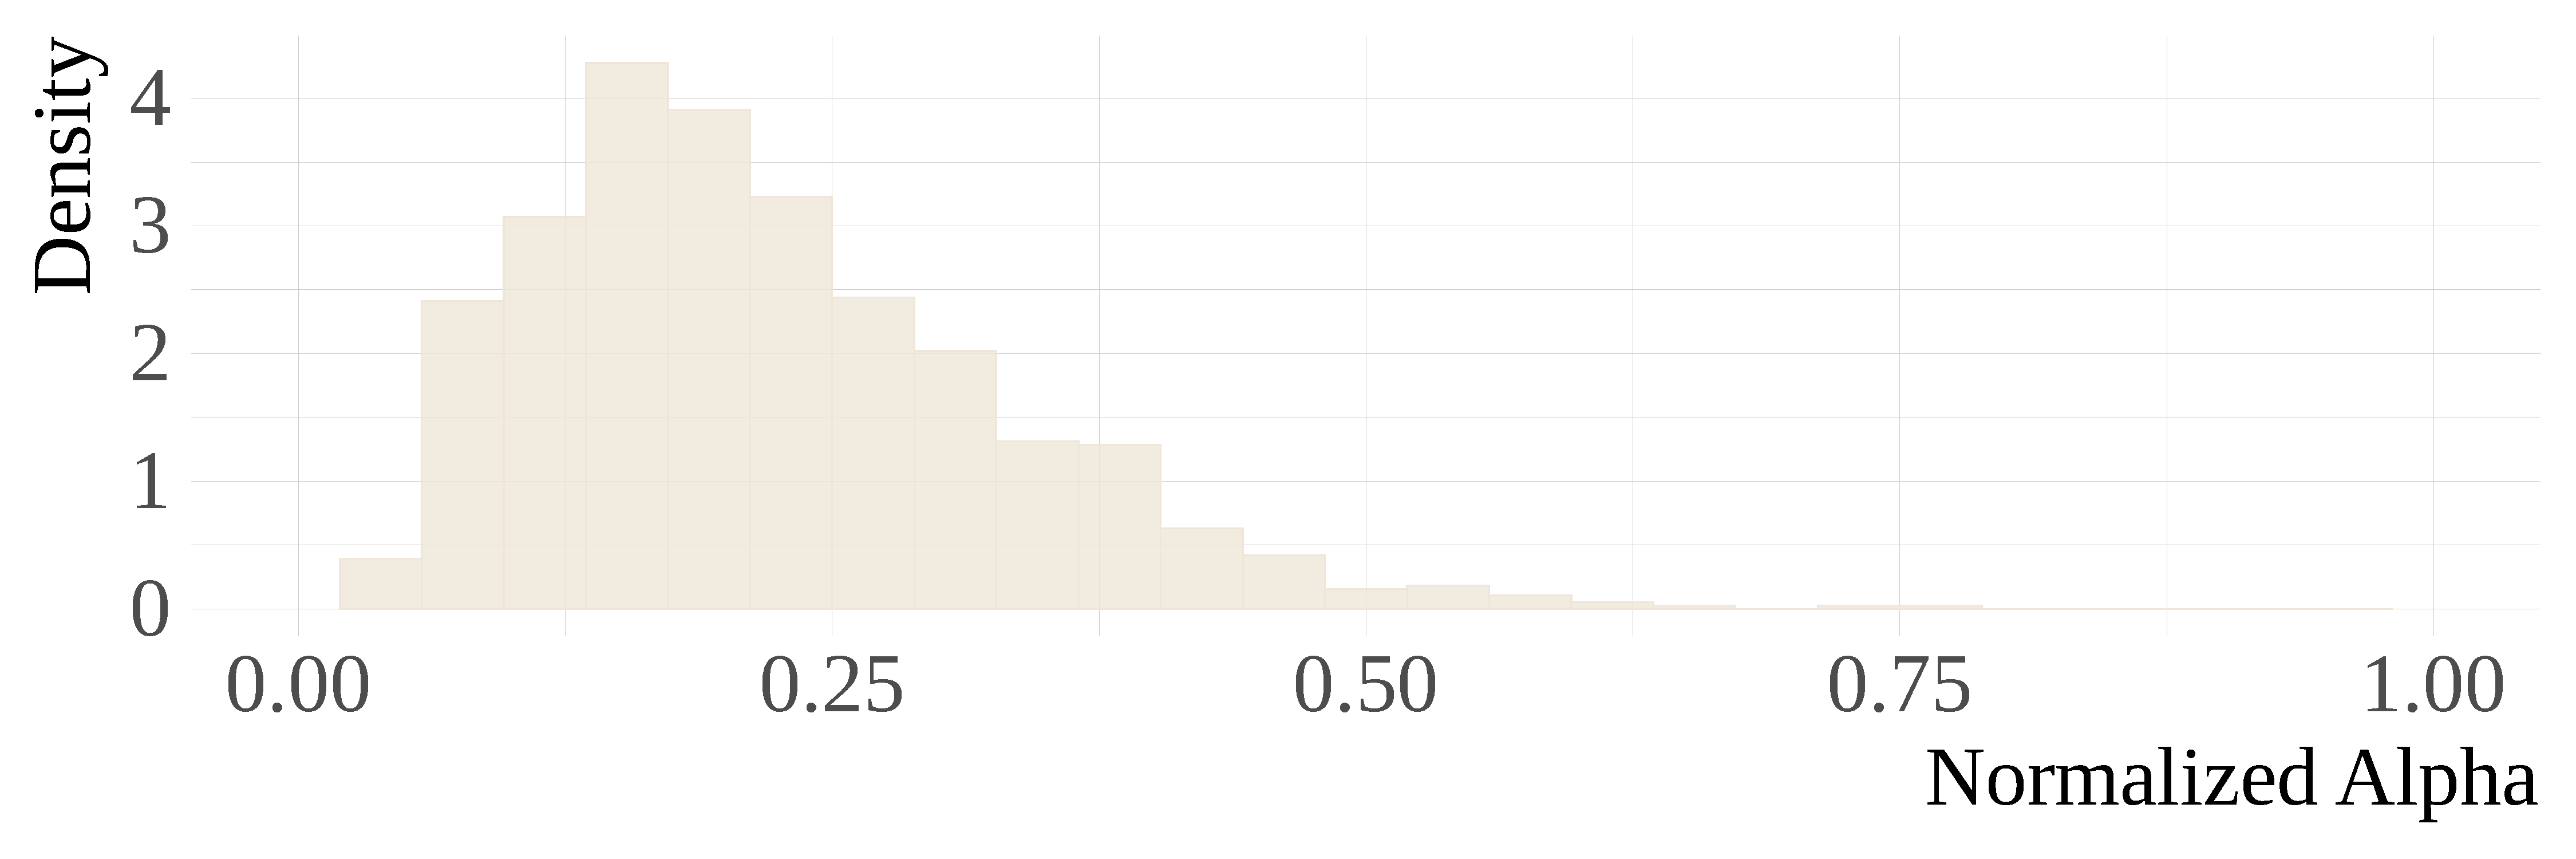
\includegraphics[width = \linewidth]{alpha_ot102_2}}
%\subcaptionbox{03 July 2016}{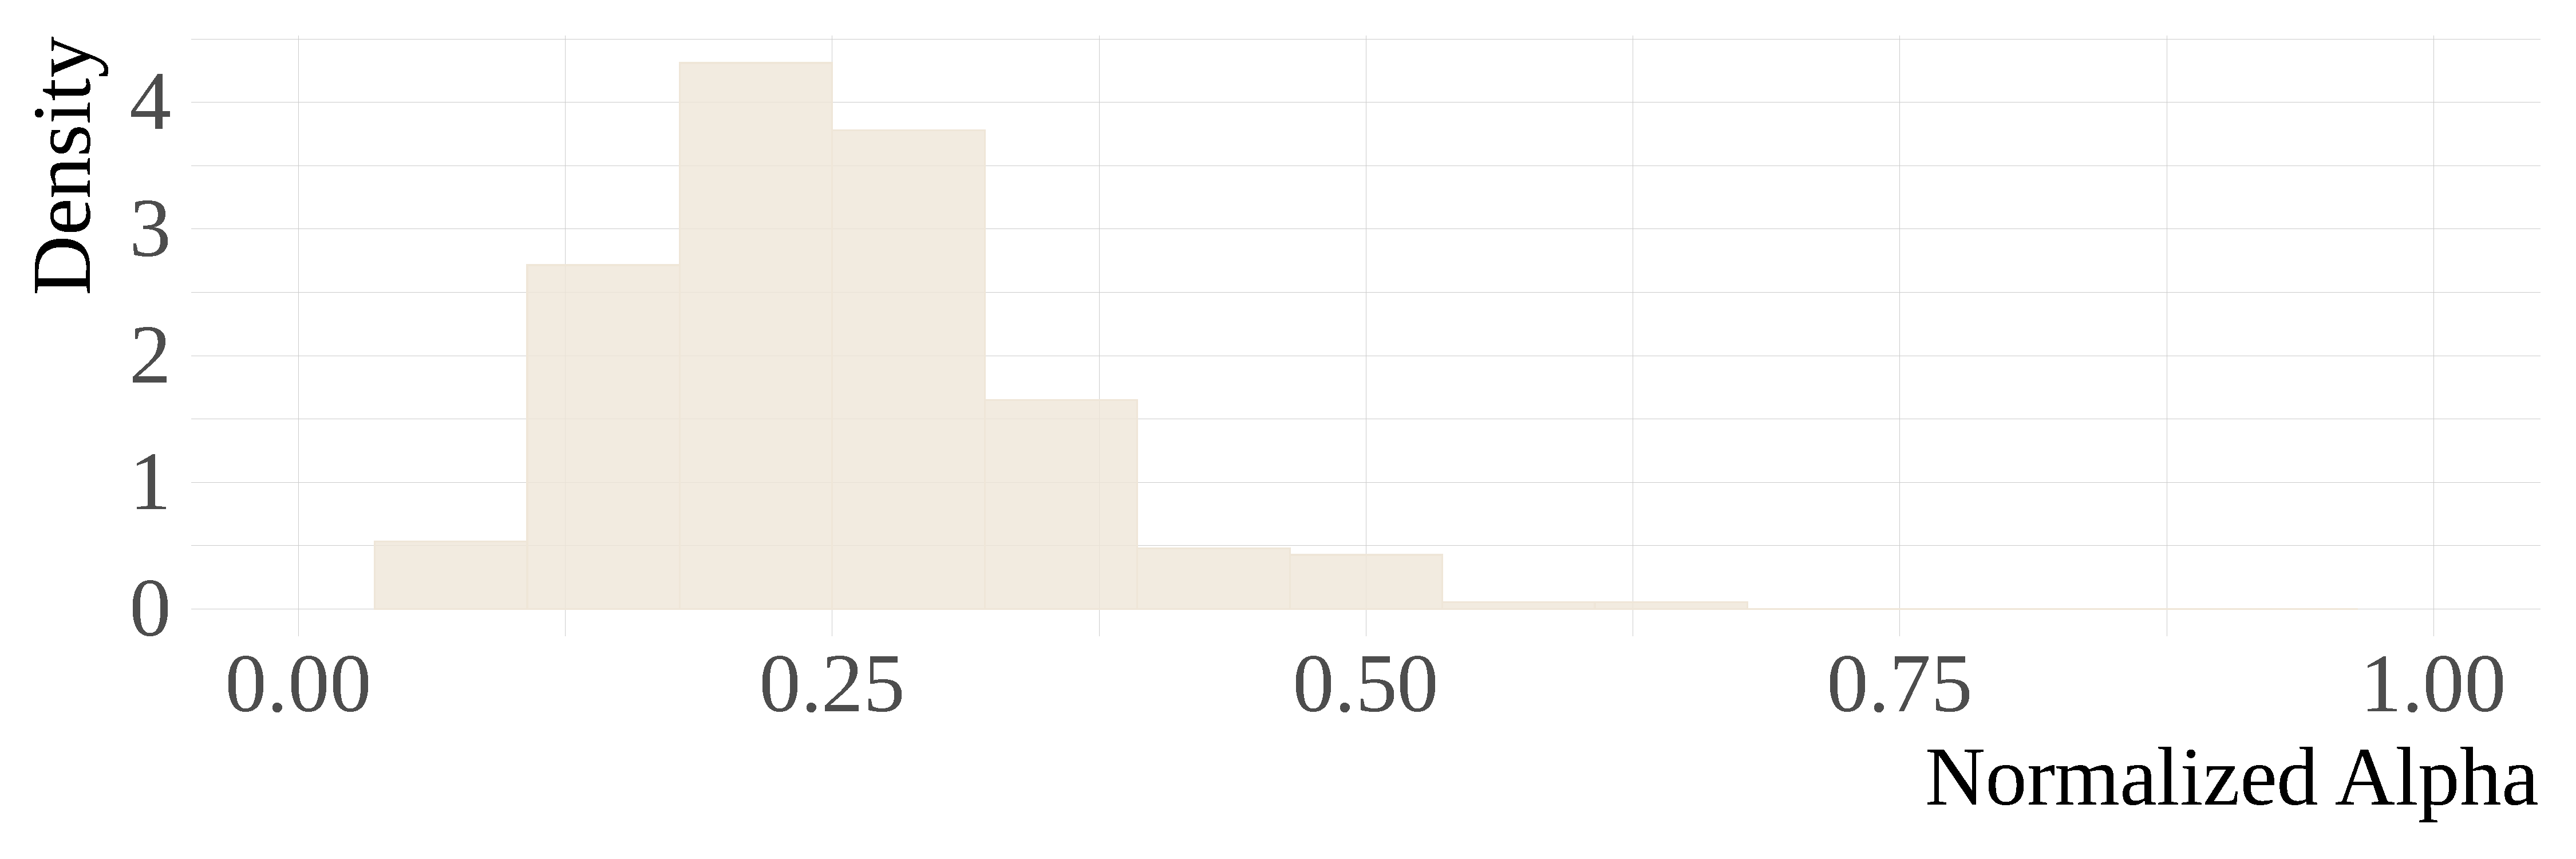
\includegraphics[width = \linewidth]{alpha_ot102_3}}
%\subcaptionbox{27 July 2016}{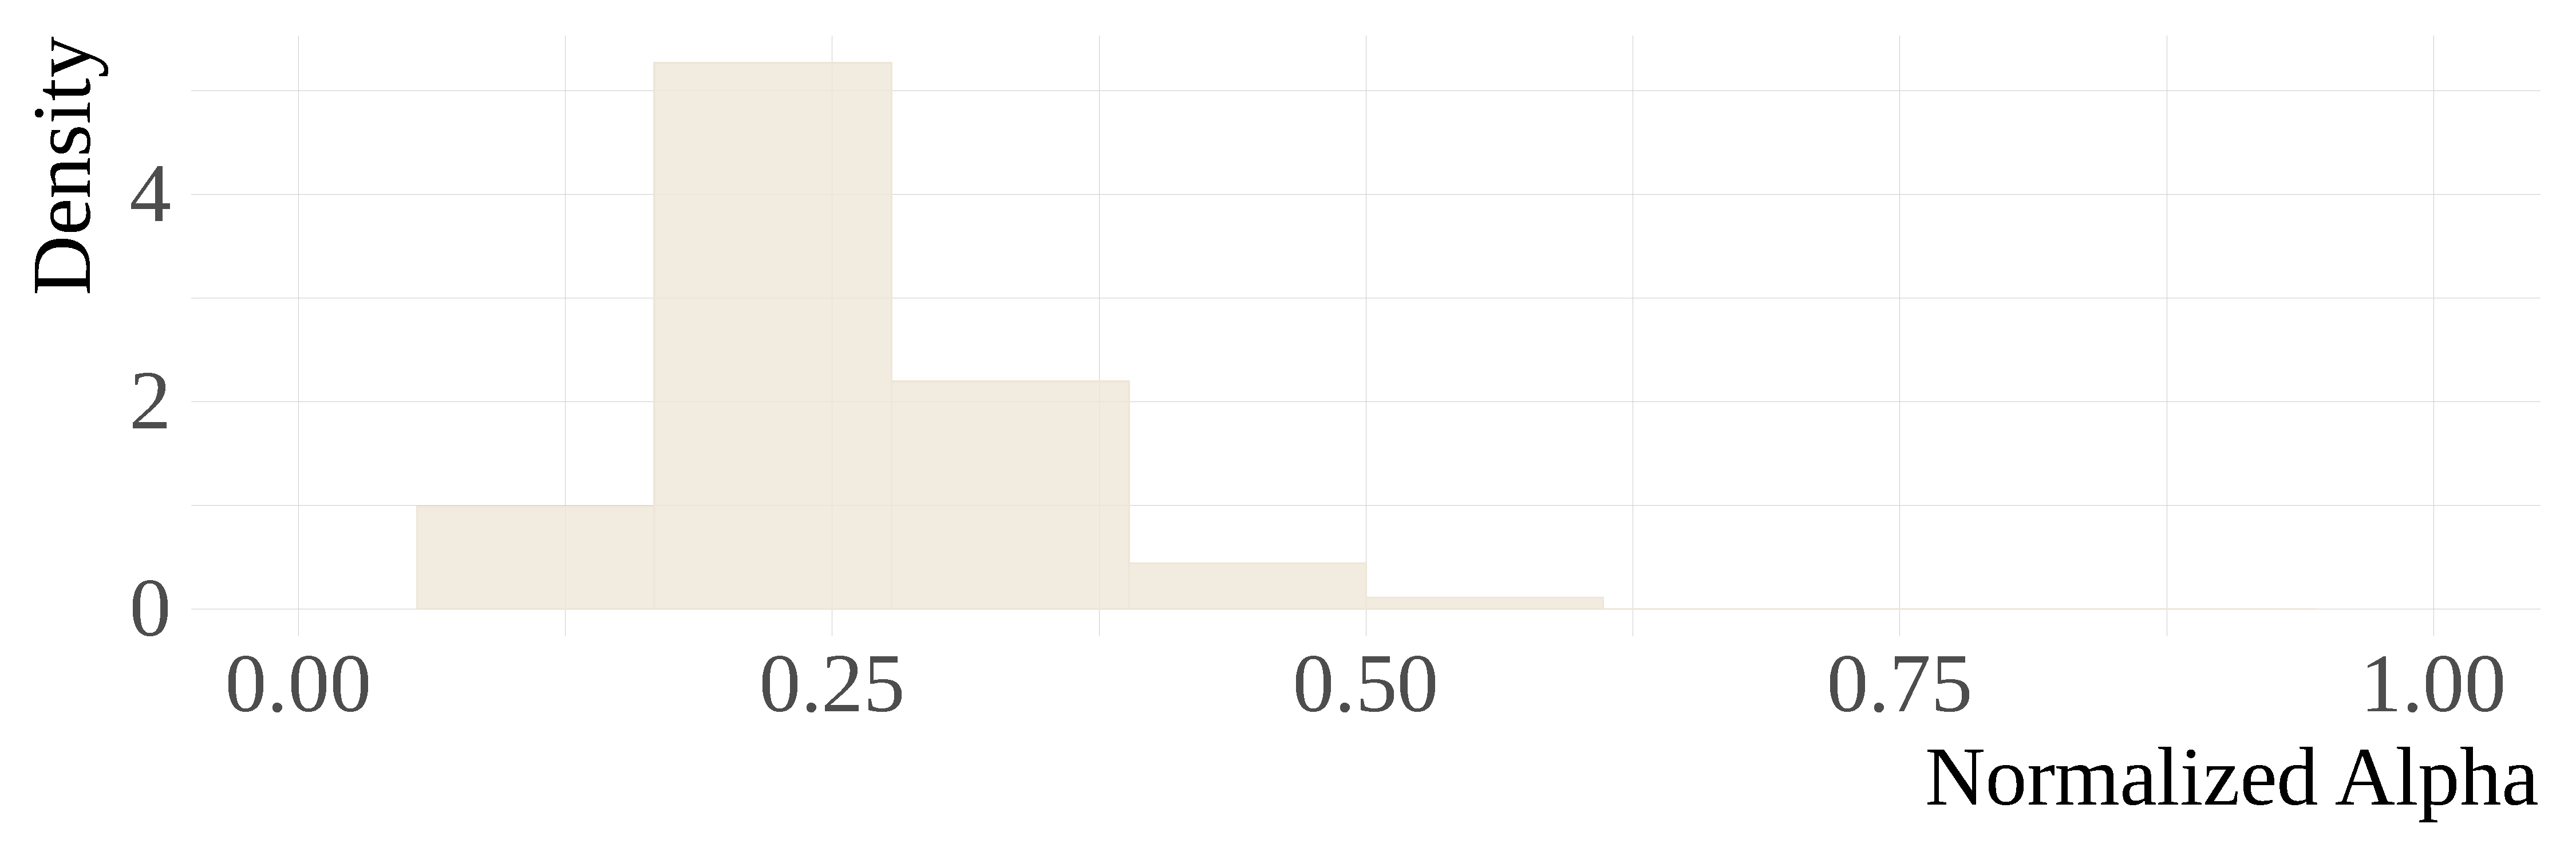
\includegraphics[width = \linewidth]{alpha_ot102_4}}
%\subcaptionbox{27 July 2016}{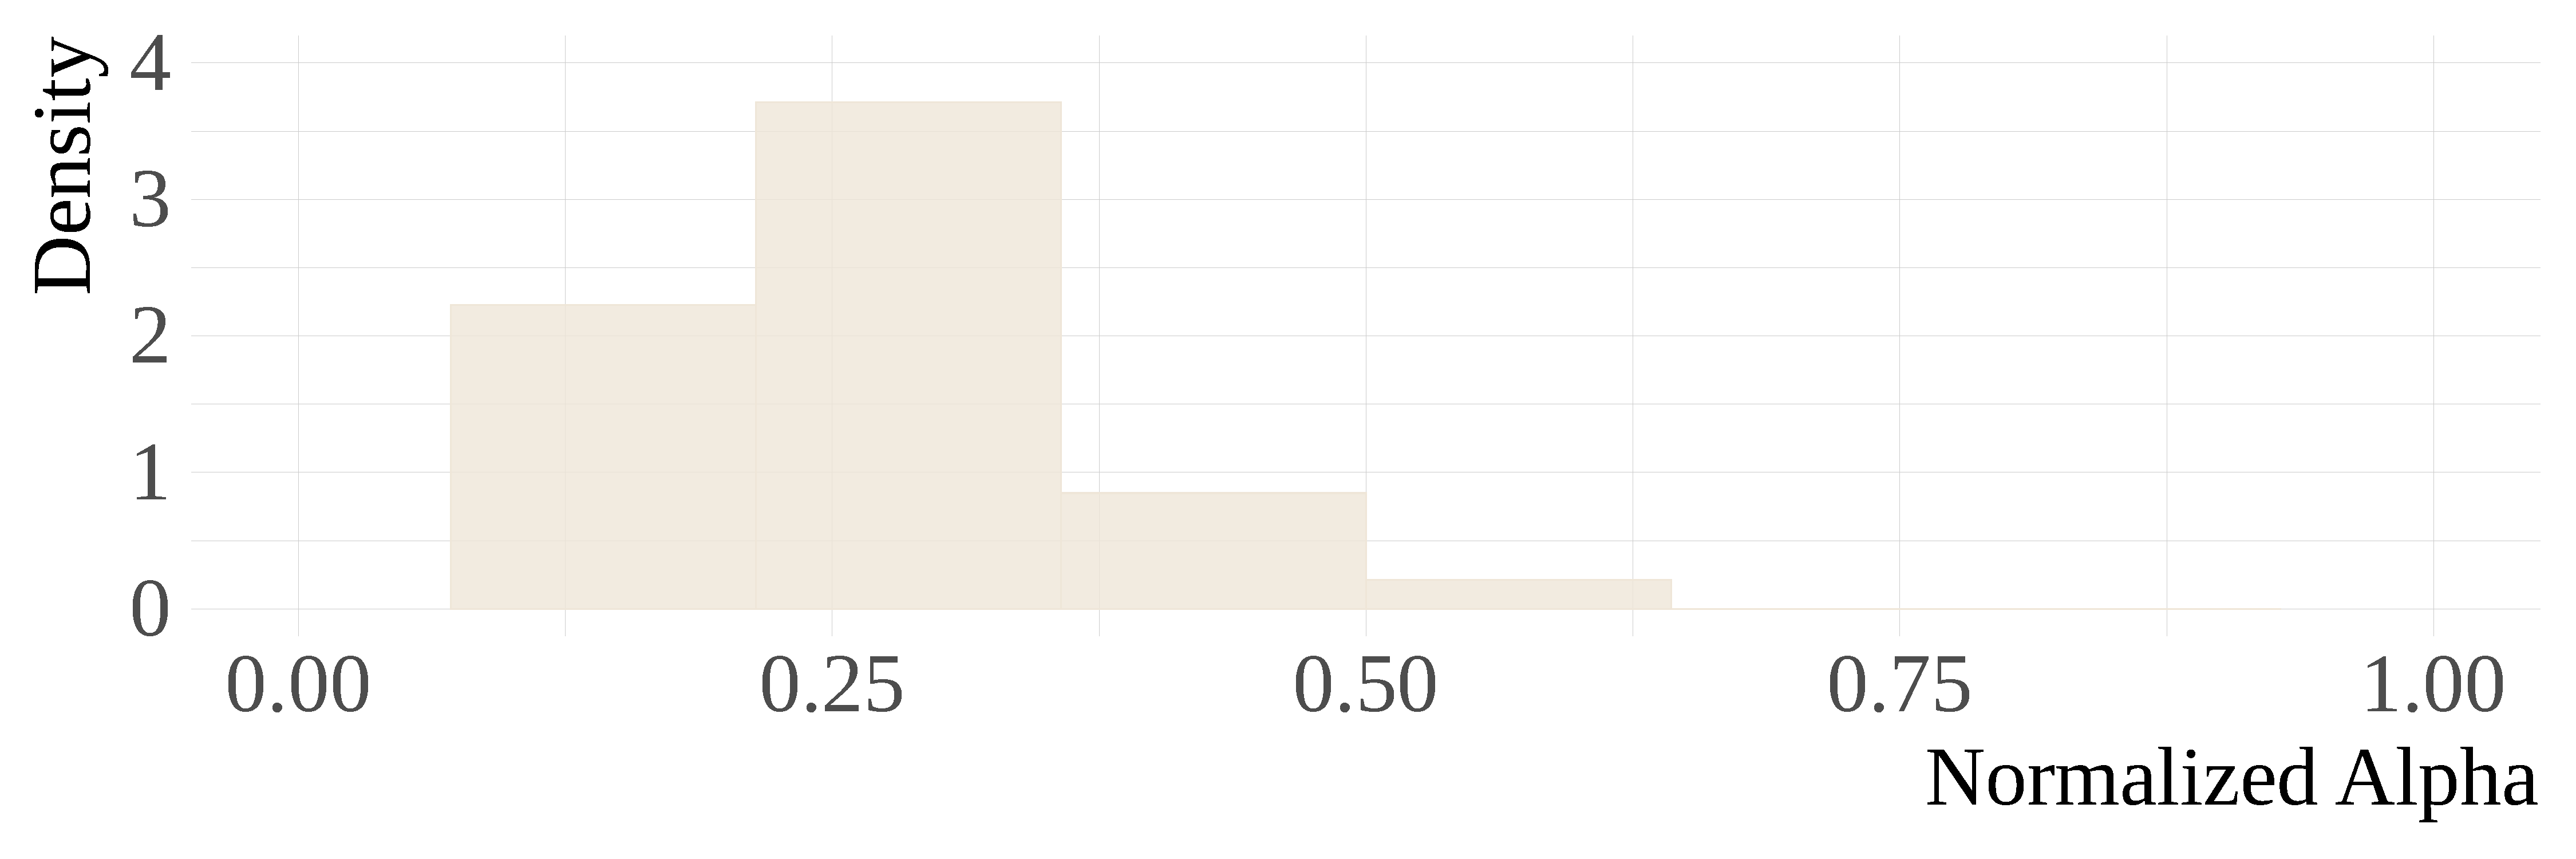
\includegraphics[width = \linewidth]{alpha_ot102_5}}
%\caption{Histograms of the geodesic distances between trihedral and the pixels from Oats 102 most similar to trihedral}
%\label{fig:histograms_alpha_ot102}
%\end{figure}

%\begin{figure}[hbt]
%\centering
%\subcaptionbox{16 May 2016}{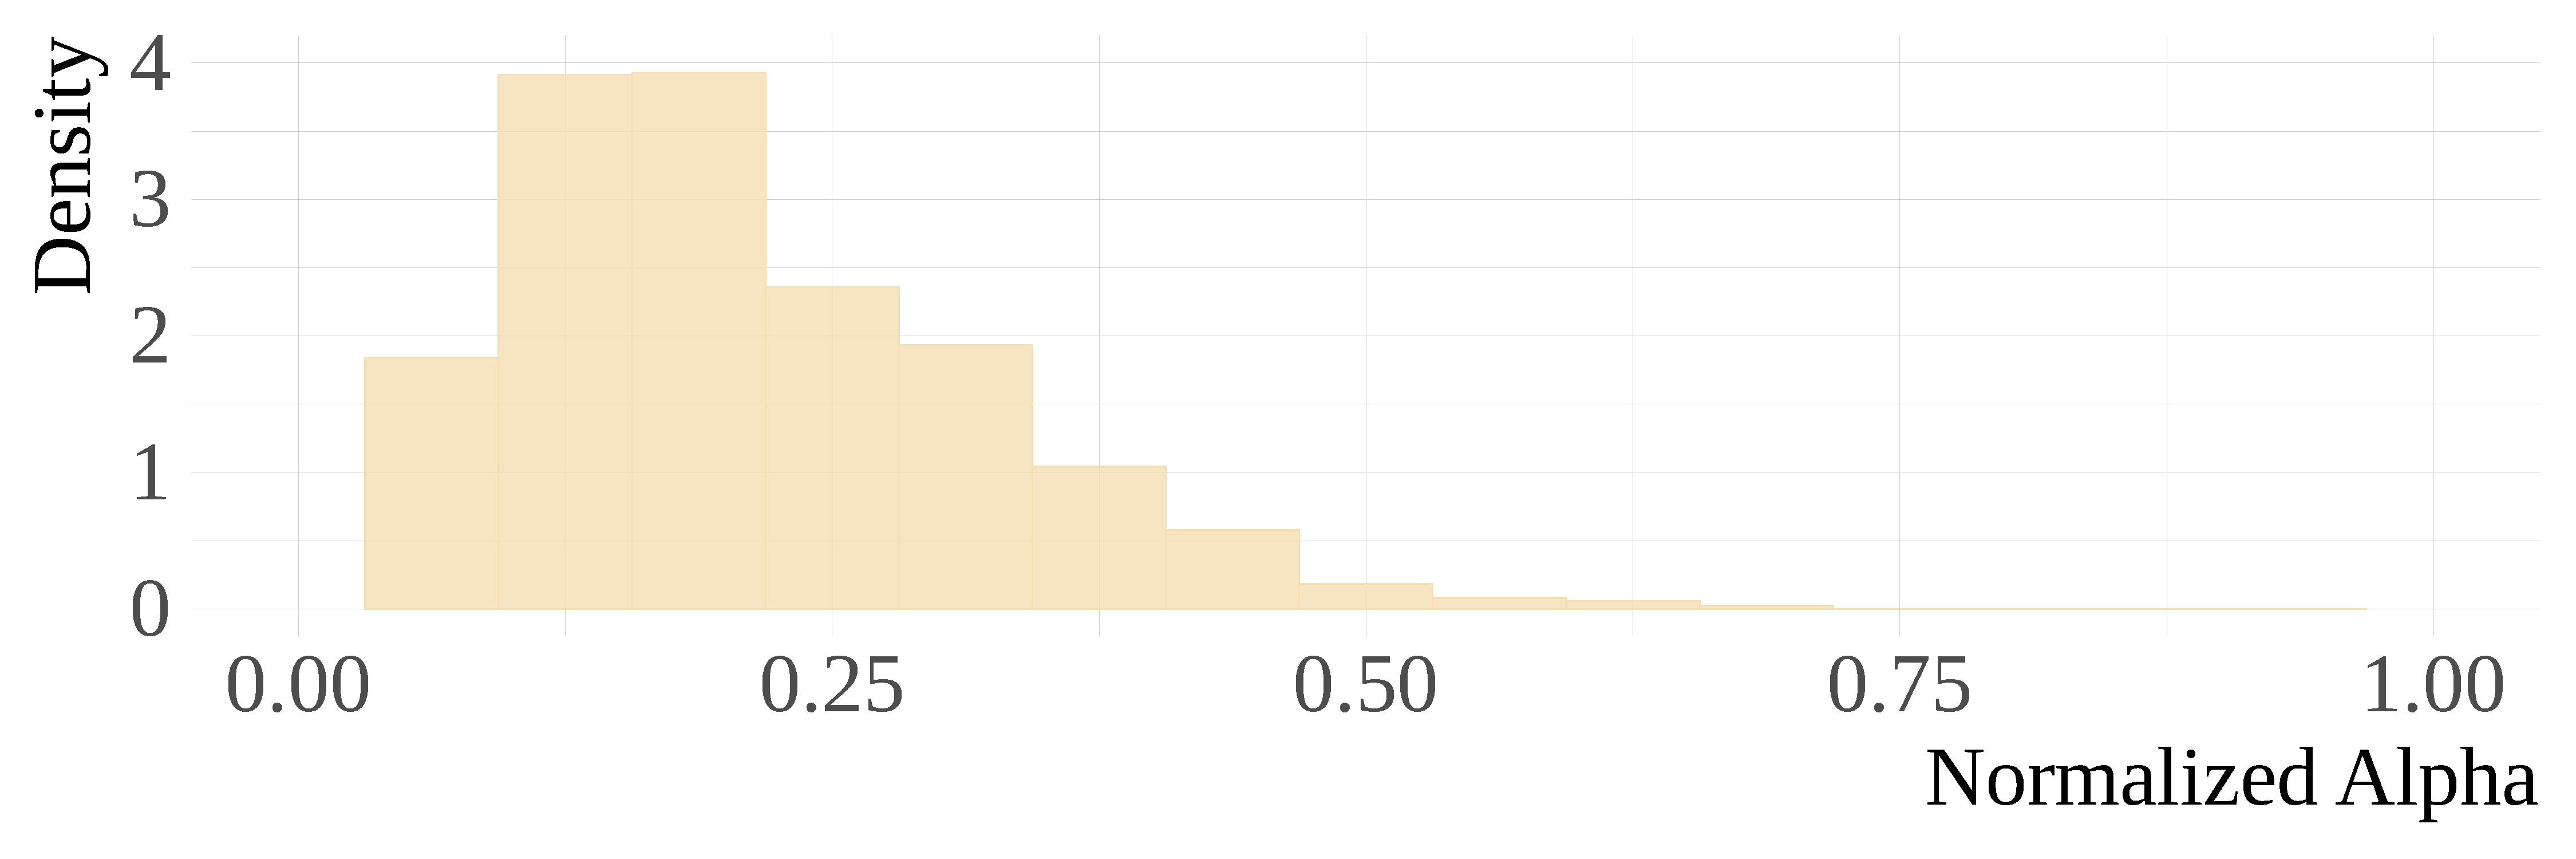
\includegraphics[width = \linewidth]{/alpha_wt104_1}}
%\subcaptionbox{09 June 2016}{\includegraphics[width = \linewidth]{/alpha_wt104_2}}
%\subcaptionbox{03 July 2016}{\includegraphics[width = \linewidth]{/alpha_wt104_3}}
%\subcaptionbox{27 July 2016}{\includegraphics[width = \linewidth]{/alpha_wt104_4}}
%\subcaptionbox{20 August 2016}{\includegraphics[width = \linewidth]{/alpha_wt104_5}}
%\caption{Histograms of the geodesic distances between trihedral and the pixels from Wheat 104 most similar to trihedral}
%\label{fig:histograms_alpha_wt104}
%\end{figure}

%Additionally, we performed a separability test based on the Hellinger distance between the original samples assuming the Beta distribution.
%Table~\ref{tab:pvalues_sep_alpha_sb231} shows the $p$-values of the null hypothesis that each pair comes from the same law.
%We observe that at level $0.05$, the only null hypothesis that cannot be rejected is that the data from the two last dates come from the same law.
%
%\begin{table}[hbt]
%  \footnotesize
%  \centering
%  \caption{$p$-values from Separability Test for normalized alpha from Soybeans 231}
%  \label{tab:pvalues_sep_alpha_sb231}
%  \begin{tabular}{ccccc}
%  \toprule
%& \textbf{09 June} & \textbf{03 July} & \textbf{27 July} & \textbf{20 Aug.}\\ \midrule
%  \textbf{16 May}  & $7.47 \times 10^{-8}$ & $9.22 \times 10^{-12}$ & $5.16 \times 10^{-21}$ & $1.31 \times 10^{-24}$ \\
%  \textbf{09 June}  & --- & $2.64 \times 10^{-3}$ & $4.55 \times 10^{-4}$ & $1.76 \times 10^{-6}$ \\
%  \textbf{03 July}  & --- & --- & $4.32 \times 10^{-2}$ & $1.07 \times 10^{-2}$\\
%  \textbf{27 July}  & --- & --- & --- & $3.64 \times 10^{-1}$ \\
%  \bottomrule
%  \end{tabular}
%\end{table}
%%
%\begin{table}[hbt]
%  \footnotesize
%  \centering
%  \caption{$p$-values from Separability Test for normalized alpha from Canola 43}
%  \label{tab:pvalues_sep_alpha_cn43}
%  \begin{tabular}{ccccc}
%  \toprule
%  & \textbf{09 June} & \textbf{03 July} & \textbf{27 July} & \textbf{20 Aug.}\\ \midrule
%  \textbf{16 May}  & $1.86 \times 10^{-19}$ & $4.07 \times 10^{-36}$ & $2.75 \times 10^{-25}$ & $9.79 \times 10^{-27}$ \\
%  \textbf{09 June}  & --- & $5.28 \times 10^{-8}$ & $2.94 \times 10^{-10}$ & $3.06 \times 10^{-10}$ \\
%  \textbf{03 July}  & --- & --- & $1.48 \times 10^{-2}$ & $3.21 \times 10^{-2}$\\
%  \textbf{27 July}  & --- & --- & --- & $9.39 \times 10^{-1}$ \\
%  \bottomrule
%  \end{tabular}
%\end{table}
%
%\begin{table}[hbt]
%  \footnotesize
%  \centering
%  \caption{$p$-values from Separability Test for normalized alpha from Oats 102}
%  \label{tab:pvalues_sep_alpha_ot102}
%  \begin{tabular}{ccccc}
%  \toprule
%  & \textbf{09 June} & \textbf{03 July} & \textbf{27 July} & \textbf{20 Aug.}\\ \midrule
%  \textbf{16 May}  & $2.77 \times 10^{-1}$ & $3.71 \times 10^{-8}$ & $2.18 \times 10^{-7}$ & $7.32 \times 10^{-7}$ \\
%  \textbf{09 June}  & --- & $2.08 \times 10^{-10}$ & $1.47 \times 10^{-8}$ & $5.45 \times 10^{-8}$ \\
%  \textbf{03 July}  & --- & --- & $1.09 \times 10^{-1}$ & $1.01 \times 10^{-1}$\\
%  \textbf{27 July}  & --- & --- & --- & $4.08 \times 10^{-1}$ \\
%  \bottomrule
%  \end{tabular}
%\end{table}
%
%\begin{table}[hbt]
%  \footnotesize
%  \centering
%  \caption{$p$-values from Separability Test for normalized alpha from Wheat 104}
%  \label{tab:pvalues_sep_alpha_wt104}
%  \begin{tabular}{ccccc}
%  \toprule
%  & \textbf{09 June} & \textbf{03 July} & \textbf{27 July} & \textbf{20 Aug.}\\ \midrule
%  \textbf{16 May}  & $4.24 \times 10^{-27}$ & $2.61 \times 10^{-24}$ & $3.08 \times 10^{-19}$ & $1.32 \times 10^{-17}$ \\
%  \textbf{09 June}  & --- & $5.42 \times 10^{-4}$ & $2.70 \times 10^{-4}$ & $5.58 \times 10^{-2}$ \\
%  \textbf{03 July}  & --- & --- & $3.31 \times 10^{-5}$ & $1.58 \times 10^{-1}$\\
%  \textbf{27 July}  & --- & --- & --- & $3.24 \times 10^{-2}$ \\
%  \bottomrule
%  \end{tabular}
%\end{table}

%In the figures \ref{fig:histograms_helicity} the histograms of normalized helicities computed for each sample are shown. For these, goodness-of-fit tests were performed -- through Komolgorov-Smirnov Test -- with Beta distribution, whose $p$-values are shown in table \ref{tab:pvalues_helicities}.

% \begin{figure}[hbt]
%     \centering
%     \subcaptionbox{16 May 2016}{\includegraphics[width = \linewidth]{Figures/Soybeans_231/helicity_sb231_1}}
%     \subcaptionbox{09 June 2016}{\includegraphics[width = \linewidth]{Figures/Soybeans_231/helicity_sb231_2}}
%     \subcaptionbox{03 July 2016}{\includegraphics[width = \linewidth]{Figures/Soybeans_231/helicity_sb231_3}}
%     \subcaptionbox{27 July 2016}{\includegraphics[width = \linewidth]{Figures/Soybeans_231/helicity_sb231_4}}
%     \subcaptionbox{20 August 2016}{\includegraphics[width = \linewidth]{Figures/Soybeans_231/helicity_sb231_5}}
%     \caption{Histograms of the normalized geodesic helicities}
%     \label{fig:histograms_helicity}
% \end{figure}

% \begin{table}[hbt]
%   \centering
%   \caption{Maximum Likelihood estimated Beta parameters for normalized helicity from Soybeans 231}
%   \label{tab:params_helicity}
%   \begin{tabular}{lrrrrr}
%     \toprule
%     \textbf{Day} & \textbf{16 May} & \textbf{09 June} & \textbf{03 July} & \textbf{27 July} & \textbf{20 Aug.}\\ 
%                  & \textbf{2016} & \textbf{2016} & \textbf{2016} & \textbf{2016} & \textbf{2016}\\\midrule
%     $\widehat{p}$ & 2.0984 & 2.4793 & 3.0300 & 2.8211 & 3.2862\\
%     $\widehat{q}$ & 26.0484 & 18.0347 & 17.0150 & 16.9940 & 17.6112\\
%     \bottomrule
%   \end{tabular}
% \end{table}


% \begin{table}[hbt]
%   \centering
%   \caption{$p$-values from Komolgorov-Smirnov Test for normalized helicity from Soybeans 231}
%   \label{tab:pvalues_helicities}
%   \begin{tabular}{lrrrrr}
%     \toprule
%     \textbf{Day} & \textbf{16 May} & \textbf{09 June} & \textbf{03 July} & \textbf{27 July} & \textbf{20 Aug.}\\
%                  & \textbf{2016} & \textbf{2016} & \textbf{2016} & \textbf{2016} & \textbf{2016}\\\midrule
%     \textbf{$p$-value} & 0.0018  & 0.0118 & 0.9812 & 0.2525 & 0.3358\\
%     \bottomrule
%   \end{tabular}
% \end{table}

\section{Conclusions}

Refs.~\cite{ClassificationPolSARGeodesic,AGeneralizedVolumeScatteringModelBasedVegetationIndexfromPolarimetricSARData2019,NovelTechniquesforBuiltupAreaExtractionfromPolarimetricSARImages2019,APolSARScatteringPowerFactorizationFrameworkandNovelRollInvariantParametersBasedUnsupervisedClassificationSchemeUsingaGeodesicDistanceinpress,ChangeDetectionPolSARGeodesicDistanceBetweenScatteringMechanisms,ARadarVegetationIndexforCropMonitoringUsingCompactPolarimetricSARData}
have shown the expressiveness and usefulness of indexes derived from Geodesic Distances, but with no assessment of their statistical properties.
This paper shows that the three main Geodesic Indexes, namely
Geodesic Purity ($P_{\text{GD}}$),
Geodesic Scattering Type Angle ($\alpha_{\text{GD}}$), and
Geodesic Helicity ($\tau_{\text{GD}}$) can be described by parsimonious and easy to use models.

The Geodesic Purity is well described by the Lognormal distribution.
This implies that the logarithmic transformation $\log P_{\text{GD}}$ can be assumed to follow a Gaussian distribution.
Both the Geodesic Scattering Type Angle and the Geodesic Helicity can be modeled by the Beta distribution.
These two models are indexed by two real parameters, with techniques readily available in most statistical software.

We used \texttt{R}~\cite{RManual} v.~3.6.3 for data processing and analysis (in particular, we used the functions provided by the \texttt{Rfast} library~\cite{Rfast} for parameter estimation), as well as for producing the graphical outputs (with the \texttt{ggplot2} library~\cite{ggplot2}).

\section*{Acknowledgment}

The authors would like to thank CNPq and Fapeal for providing partial support to this research.

\bibliographystyle{IEEEtran}
\bibliography{references}

\end{document}